
\chapter{Teoria}

\section{Cap al concepte de vector}

La paraula «vector» és coneguda per tothom en geometria. Al batxillerat s’estudien els vectors de la geometria plana i de l’espai. Tanmateix, en matemàtiques hi ha moltes altres classes d’objectes que es comporten de la mateixa manera; això vol dir que comparteixen unes mateixes propietats bàsiques. Descobrir aquestes propietats és el primer pas cap a la \textbf{generalització}.

El segon pas és la \textbf{axiomatització}: triar, entre totes les propietats observades, aquelles a partir de les quals es poden deduir totes les altres. Aquestes propietats fonamentals s’anomenen \textbf{axiomes}. Qualsevol classe d’objectes que satisfaci aquests axiomes es dirà que es comporta com els vectors.

El darrer pas és desenvolupar la \textbf{teoria matemàtica} a partir dels axiomes triats. Els resultats que s’obtenen d’aquesta teoria constitueixen les propietats generals dels vectors. Per tant, qualsevol classe d’objectes que es comporti com els vectors tindrà aquestes propietats.

Segons aquesta teoria, anomenarem \textbf{vector} qualsevol element d’un espai vectorial. Cal, doncs, definir el concepte d’espai vectorial.

\section{Concepte d’espai vectorial}

Per saber si un conjunt és un espai vectorial, cal comprovar que s’hi poden definir dues operacions. La primera és interna: la suma de dos elements del conjunt torna a ser un element del conjunt. La segona és externa: el producte d’un escalar d’un cos commutatiu per un element del conjunt torna a ser un element del conjunt. A més, aquestes dues operacions han de satisfer unes propietats determinades, anomenades axiomes.

\begin{definicio}
Donat un cos commutatiu $\mathbb{K}$, sigui $E$ un conjunt arbitrari d’objectes sobre els quals es defineixen dues operacions: l’addició i la multiplicació per escalars, és a dir, per elements de $\mathbb{K}$. Per \textbf{addició} entenem una regla que associa a cada parella d’objectes $\mathbf{u}$ i $\mathbf{v}$ de $E$ un element $\mathbf{u}+\mathbf{v}$, anomenat \textbf{suma} de $\mathbf{u}$ i $\mathbf{v}$. Per \textbf{multiplicació per escalars} entenem una regla que associa a cada escalar $\lambda\in\mathbb{K}$ i a cada objecte $\mathbf{u}$ de $E$ un element $\lambda\mathbf{u}$, anomenat \textbf{producte} de $\mathbf{u}$ per l’escalar $\lambda$. Si els axiomes següents són satisfets per tots els objectes $\mathbf{u},\mathbf{v},\mathbf{w}\in E$ i tots els escalars $\lambda,\mu\in\mathbb{K}$, aleshores $E$ rep el nom d’\textbf{espai vectorial sobre} $\mathbb{K}$, i els objectes de $E$ s’anomenen \textbf{vectors}.

\begin{enumerate}
\item Si $\mathbf{u}$ i $\mathbf{v}$ són objectes de $E$, aleshores $\mathbf{u}+\mathbf{v}$ és a $E$; és a dir, l’addició és una operació interna.
\item $\mathbf{u}+(\mathbf{v}+\mathbf{w})=(\mathbf{u}+\mathbf{v})+\mathbf{w}$; l’addició és associativa.
\item $\mathbf{u}+\mathbf{v}=\mathbf{v}+\mathbf{u}$; l’addició és commutativa.
\item Existeix un objecte $\mathbf{0}$ de $E$, anomenat \textbf{vector zero}, tal que $\mathbf{0}+\mathbf{u}=\mathbf{u}+\mathbf{0}=\mathbf{u}$; l’addició té element neutre.
\item Per a cada $\mathbf{u}$ de $E$, existeix un objecte $-\mathbf{u}$ de $E$, anomenat \textbf{oposat} de $\mathbf{u}$, tal que $\mathbf{u}+(-\mathbf{u})=(-\mathbf{u})+\mathbf{u}=\mathbf{0}$; l’addició té element simètric.
\item Si $\lambda\in\mathbb{K}$ i $\mathbf{u}\in E$, aleshores $\lambda\mathbf{u}\in E$; és a dir, la multiplicació per escalars és una operació externa i el conjunt d’operadors és $\mathbb{K}$.
\item $\lambda (\mathbf{u}+\mathbf{v})=\lambda \mathbf{u}+\lambda \mathbf{v}$.
\item $(\lambda +\mu )\mathbf{u}=\lambda \mathbf{u}+\mu \mathbf{u}$.
\item $\lambda (\mu \mathbf{u})=(\lambda \mu )\mathbf{u}$.
\item $1\mathbf{u}=\mathbf{u}$, on $1$ és la unitat del cos $\mathbb{K}$.
\end{enumerate}
\end{definicio}

\begin{observacio}
Fem les observacions importants següents:

\begin{enumerate}
\item En la teoria d’espais vectorials, el cos $\mathbb{K}$ es fixa d’una vegada per sempre i s’anomena \textbf{cos base}. Els seus elements s’anomenen \textbf{escalars} i es designen habitualment amb lletres gregues.
\item Els elements dels espais vectorials s’anomenen \textbf{vectors} i es designen habitualment amb lletres minúscules en negreta. Per distingir el conjunt de la seva estructura d’espai vectorial, utilitzarem la notació que convingui en cada context.
\item En realitat, la distinció entre escalars i vectors no té cap sentit matemàtic absolut: com veurem més avall, els escalars també es poden comportar com a vectors.
\item S’ha utilitzat el mateix signe $+$ per denotar dues operacions diferents: l’addició en $\mathbb{K}$ i l’addició en l’espai vectorial. Això no dona lloc a confusió si ens fixem en els elements que uneix el signe $+$. El mateix es pot dir de la multiplicació en $\mathbb{K}$ i de la multiplicació per escalars.
\item El conjunt $E$, dotat de l’addició, té estructura de \textbf{grup commutatiu o abelià} quan satisfà els axiomes 1--5. En aquesta secció suposa que el lector coneix les propietats elementals de la teoria de grups.
\item En particular, un espai vectorial sobre el cos $\mathbb{R}$ dels nombres reals s’anomena \textbf{espai vectorial real}, i un espai vectorial sobre el cos $\mathbb{C}$ dels nombres complexos s’anomena \textbf{espai vectorial complex}.
\item Cal tenir present que, en la definició d’espai vectorial, no s’especifica la naturalesa dels objectes que anomenem vectors ni la de les operacions que anomenem addició i multiplicació per escalars. Qualsevol classe d’objectes pot servir com a vectors, sempre que satisfaci els axiomes dels espais vectorials. Els exemples següents mostren una part de la diversitat d’espais vectorials possibles.
\end{enumerate}
\end{observacio}

\begin{exemple}
Tot cos commutatiu és un espai vectorial sobre si mateix, el que
mostra que els ``escalars'' són en aquest cas també ``vectors''; $%
\mathbb{Q}$, $\mathbb{R}$ i $\mathbb{C}$ són espais vectorials sobre si mateix.
\end{exemple}

\begin{exemple}
El cos dels nombres reals $\mathbb{R}$ és un espai vectorial
sobre el cos $\mathbb{Q}$ dels nombres racionals; $\sqrt{2},\pi ,5%
\sqrt{2}+\pi /3$, etc., són vectors d’aquest espai.
\end{exemple}

\begin{exemple}
Prenem $E=\mathbb{C}$, $\mathbb{K}=\mathbb{R}$ i les operacions%
\begin{equation*}
(a+bi)+(c+di)=(a+c)+(b+d)i
\end{equation*}%
\begin{equation*}
\lambda (a+bi)=\lambda a+\lambda bi
\end{equation*}%
on $a,b,c,d,\lambda \in \mathbb{R}$, aleshores $\mathbb{C}$ és un espai
vectorial real; és també un espai vectorial sobre si mateix. És important saber que aquestes dues estructures són diferents.
\end{exemple}

\begin{exemple}
Prenem $\mathbb{K}=\mathbb{R}$ i com $E$ el conjunt dels vectors de
origen donat $O$ de l’espai ordinari. Definim la suma de dos vectors per
la regla del paral·lelogram i el producte d’un nombre real $\lambda $
per un vector $\mathbf{v}$ com el vector obtingut aplicant a $\mathbf{v}$
la homotècia de centre $O$ i raó $\lambda $. D’aquesta manera s’obté
un espai vectorial real. En aquest exemple està l’origen de la noció general d’espai vectorial i explica a més l'ús de la paraula
``vector'' per designar els seus elements.
\end{exemple}

\begin{center}
\definecolor{figA}{HTML}{B02438}\definecolor{figB}{HTML}{27476E}%
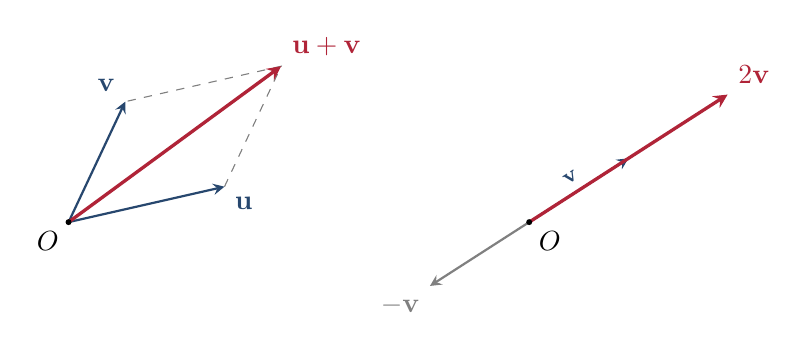
\begin{tikzpicture}[scale=0.9,>=stealth]
% Suma: regla del paral·lelogram
\coordinate (O) at (0,0);
\coordinate (U) at (2.2,0.5);
\coordinate (V) at (0.8,1.7);
\coordinate (S) at (3.0,2.2);
\draw[dashed,gray] (U) -- (S) -- (V);
\draw[->,thick,figB] (O) -- (U) node[below right]{$\mathbf{u}$};
\draw[->,thick,figB] (O) -- (V) node[above left]{$\mathbf{v}$};
\draw[->,very thick,figA] (O) -- (S) node[above right]{$\mathbf{u}+\mathbf{v}$};
\fill (O) circle (1.2pt) node[below left]{$O$};
% Homotècia: producte per un escalar
\begin{scope}[xshift=6.5cm]
\coordinate (O2) at (0,0);
\draw[->,thick,figB] (O2) -- (1.4,0.9) node[midway,above,sloped]{\footnotesize $\mathbf{v}$};
\draw[->,very thick,figA] (O2) -- (2.8,1.8) node[above right]{$2\mathbf{v}$};
\draw[->,thick,gray] (O2) -- (-1.4,-0.9) node[below left]{$-\mathbf{v}$};
\fill (O2) circle (1.2pt) node[below right]{$O$};
\end{scope}
\end{tikzpicture}

{\small\itshape La suma per la regla del paral·lelogram i el producte per un escalar com a homotècia de centre $O$.}
\end{center}

Abans de començar, val la pena preguntar-se on són els espais vectorials
avui. La resposta és: pertot arreu on hi hagi informació que es pugui sumar
i escalar. Una imatge digital en escala de grisos de $1000\times 1000$
píxels és un vector de $\mathbb{R}^{1000000}$, i operacions tan quotidianes
com apujar la brillantor o fondre dues imatges són, exactament, el producte
per un escalar i la suma de vectors. Els missatges que viatgen per la xarxa
es protegeixen amb codis correctors d'errors, que són subespais vectorials
de $(\mathbb{Z}_{2})^{n}$; per això en aquesta unitat treballarem també
sobre cossos finits. Les solucions d'un sistema d'equacions lineals
homogeni, o d'una equació diferencial lineal homogènia, formen un espai
vectorial: trobar-ne una base és resoldre'ls tots de cop. I cada fotograma
d'un videojoc en tres dimensions es calcula aplicant canvis de base com els
que estudiarem al final del capítol. El llenguatge que introduïm a
continuació és, doncs, el llenguatge comú de tots aquests problemes.

\begin{exemple}
S’anomena \textbf{vector d’ordre} $n$ \textbf{sobre} $\mathbb{K}$ a tota $n$-%
tupla ordenada $(x_{1},...,x_{n})$ d’elements del cos commutatiu $%
\mathbb{K}$. Els elements $x_{i}$ s’anomenen \textbf{components} del
vector. L’element $x_{i}$ rep aleshores el nom de component $i$-èsima del vector. Dos vectors d’ordre $n$ són iguals si i només si
els seus components són iguals. Distingirem entre \textbf{vector fila}%
\begin{equation*}
(%
\begin{array}{ccc}
x_{1} & \cdots & x_{n}%
\end{array}%
)
\end{equation*}%
i \textbf{vector columna}%
\begin{equation*}
\left( 
\begin{array}{c}
x_{1} \\ 
\vdots \\ 
x_{n}%
\end{array}%
\right)
\end{equation*}%
És fàcil dotar el conjunt d’aquests vectors d'estructura d’espai
vectorial sobre $\mathbb{K}$. L'addició es defineix per 
\begin{equation*}
(x_{1},...,x_{n})+(y_{1},...,y_{n})=(x_{1}+y_{1},...,x_{n}+y_{n})
\end{equation*}%
L’element neutre és $\mathbf{0}=(0,...,0)$ i l'oposat de $%
(x_{1},...,x_{n})$ és $(-x_{1},...,-x_{n})$. La multiplicació per un
escalar $\lambda \in \mathbb{K}$ es defineix per%
\begin{equation*}
\lambda (x_{1},...,x_{n})=(\lambda x_{1},...,\lambda x_{n})
\end{equation*}%
És immediat comprovar que es compleixen tots els axiomes d’espai
vectorial, ja que es redueixen a les propietats elementals entre
elements del cos $\mathbb{K}$. Aquest espai vectorial es denota per $%
\mathbb{K}^{n}$. Aquest exemple té el seu origen en la geometria analítica, en representar un vector pels seus components en els eixos de coordenades.
\end{exemple}

\begin{exemple}
El conjunt 
\begin{equation*}
\mathbb{R}_{n}\left[ x\right] =\left\{
a_{0}+a_{1}x+a_{2}x^{2}+...+a_{n}x^{n}:a_{0},a_{1},a_{2},...,a_{n}\in 
\mathbb{R}\right\}
\end{equation*}%
dels polinomis de grau com a màxim $n$ amb coeficients reals i les
operacions%
\begin{equation*}
(a_{0}+a_{1}x+a_{2}x^{2}+...+a_{n}x^{n})+(b_{0}+b_{1}x+b_{2}x^{2}+...+b_{n}x^{n})=
\end{equation*}%
\begin{equation*}
(a_{0}+b_{0})+(a_{1}+b_{1})x+(a_{2}+b_{2})x^{2}+...+(a_{n}+b_{n})x^{n}
\end{equation*}%
\begin{equation*}
\lambda (a_{0}+a_{1}x+a_{2}x^{2}+...+a_{n}x^{n})=\lambda a_{0}+\lambda
a_{1}x+\lambda a_{2}x^{2}+...+\lambda a_{n}x^{n}
\end{equation*}%
formen un espai vectorial real.
\end{exemple}

\begin{exemple}
El conjunt $\mathcal{F}(\mathbb{R},\mathbb{R})=\left\{ f:f:\mathbb{R}%
\rightarrow \mathbb{R}\right\} $ de les funcions reals de variable real i
les operacions $(f,g)\longmapsto f+g$ i $(\lambda ,f)\longmapsto \lambda f$
definides com segueix%
\begin{align*}
(f+g)(x) &=f(x)+g(x) \\
(\lambda f)(x) &=\lambda f(x)
\end{align*}%
formen un espai vectorial real.
\end{exemple}

\begin{exemple}
El conjunt $\mathcal{M}_{n\times m}(\mathbb{R})$ de les matrius d’ordre $%
n\times m$ amb coeficients reals juntament amb les operacions d'addició
matricial i multiplicació escalar:%
\begin{align*}
(a_{ij})+(b_{ij}) &=(a_{ij}+b_{ij}) \\
\lambda (a_{ij}) &=(\lambda a_{ij})
\end{align*}%
on $1\leq i\leq n$ i $1\leq j\leq m$, formen un espai vectorial real.
\end{exemple}

\begin{exemple}
El conjunt $E$ de tots els punts del pla que es troben en el primer
quadrant no és un espai vectorial real. Per veure-ho, observeu que
el punt de coordenades $(1,1)$ està en $E$, però $(-1)(1,1)=(-1,-1)$ no
hi és.
\end{exemple}

\begin{center}
\definecolor{figA}{HTML}{B02438}\definecolor{figB}{HTML}{27476E}%
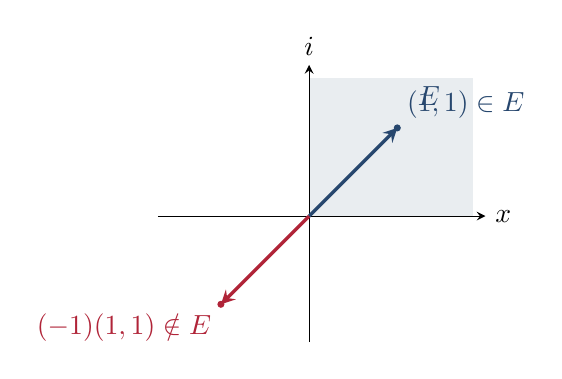
\begin{tikzpicture}[scale=0.8,>=stealth]
\fill[figB!10] (0,0) rectangle (2.6,2.2);
\draw[->] (-2.4,0) -- (2.8,0) node[right]{$x$};
\draw[->] (0,-2.0) -- (0,2.4) node[above]{$i$};
\node[figB] at (1.9,1.9) {$E$};
\draw[->,very thick,figB] (0,0) -- (1.4,1.4);
\fill[figB] (1.4,1.4) circle (1.6pt) node[above right]{$(1,1)\in E$};
\draw[->,very thick,figA] (0,0) -- (-1.4,-1.4);
\fill[figA] (-1.4,-1.4) circle (1.6pt) node[below left]{$(-1)(1,1)\notin E$};
\end{tikzpicture}

{\small\itshape El primer quadrant no és tancat pel producte per escalars negatius.}
\end{center}

\begin{exemple}
El conjunt dels polinomis de segon grau amb coeficients reals no és
un espai vectorial real. Per veure-ho, considerem els següents
polinomis de segon grau:%
\begin{equation*}
p(x)=x^{2}\text{ \ \ i \ \ }q(x)=-x^{2}+x+1
\end{equation*}%
Aleshores, la seva suma no és un polinomi de segon grau, ja que%
\begin{equation*}
p(x)+q(x)=x+1
\end{equation*}
\end{exemple}

\begin{observacio}
Seria interessant que el lector provés tots els axiomes dels
espais vectorials en els exemples anteriors; és fàcil, encara que una mica
llarg.
\end{observacio}

\section{Propiedades elementals}

Com a conseqüència de la definició, s’obté els següents
resultats.

\begin{teorema}
Per a qualsevol $\mathbf{u}$ de $E$ i $\lambda $ de $\mathbb{K}$, es
compleix:

\begin{enumerate}
\item $0\mathbf{u}=\mathbf{0}$

\item $\lambda \mathbf{0}=\mathbf{0}$

\item $\lambda \mathbf{u}=\mathbf{0}$ implica $\lambda =0$ o $\mathbf{u}=%
\mathbf{0}$

\item $(-1)\mathbf{u}=-\mathbf{u}$
\end{enumerate}

\end{teorema}
\begin{prova}
\bigskip (1.) En efecte, aplicant el axioma 8, es té%
\begin{equation*}
0\mathbf{u}=(0+0)\mathbf{u}=0\mathbf{u}+0\mathbf{u}
\end{equation*}%
i, d’aquí, sumant a ambdós membres l'oposat de $0\mathbf{u}$
(cancel·lació), es dedueix $0\mathbf{u}=\mathbf{0}$.

(2.) En efecte, aplicant els axiomes 4 i 7, es té%
\begin{equation*}
\lambda \mathbf{0}=\lambda (\mathbf{0}+\mathbf{0})=\lambda \mathbf{0}%
+\lambda \mathbf{0}
\end{equation*}%
i, d’aquí, per la mateixa raó de abans, es dedueix $\lambda \mathbf{%
0}=\mathbf{0}$.

(3.) En efecte, si $\lambda \neq 0$, $\lambda $ és invertible en $\mathbb{K}$%
. Aleshores, aplicant el axioma 9 i l’apartat anterior, es té%
\begin{equation*}
\mathbf{u}=1\mathbf{u}=(\lambda ^{-1}\lambda )\mathbf{u}=\lambda
^{-1}(\lambda \mathbf{u})=\lambda ^{-1}\mathbf{0}=\mathbf{0}
\end{equation*}%
i d’aquí, es dedueix el que volíem demostrar.

(4.) En efecte, aplicant els axiomes 10 i 8, i l’apartat 1, es té 
\begin{equation*}
\mathbf{u}+(-1)\mathbf{u}=1\mathbf{u}+(-1)\mathbf{u}=(1+(-1))\mathbf{u}=0%
\mathbf{u}=\mathbf{0}
\end{equation*}%
d’on, per la unicitat de l’oposat de $\mathbf{u}$, es té el que volíem provar.
\end{prova}

\section{Producte d’espais vectorials}

El procediment que ens ha permès definir $\mathbb{K}^{n}$ a partir de $%
\mathbb{K}$ pot generalizarse per a construir nous espais a partir de
espais coneguts.

Siguin $E_{1}$ i $E_{2}$ dos espais vectorials sobre el
mateix cos commutatiu $\mathbb{K}$. Considerem el conjunt producte $%
E_{1}\times E_{2}$ i les dues operacions següents:%
\begin{align*}
(\mathbf{u}_{1},\mathbf{u}_{2})+(\mathbf{v}_{1},\mathbf{v}_{2}) &=(\mathbf{u%
}_{1}+\mathbf{v}_{1},\mathbf{u}_{2}+\mathbf{v}_{2}) \\
\lambda (\mathbf{u}_{1},\mathbf{u}_{2}) &=(\lambda \mathbf{u}_{1},\lambda 
\mathbf{u}_{2})
\end{align*}%
Aleshores amb aquests datos tenim un espai vectorial sobre $\mathbb{K}$ que
s’anomena \textbf{espai vectorial producte} $E_{1}\times E%
_{2}$.

De la mateixa manera es defineix el producte de $n$ espais vectorials $E%
_{1},...,E_{n}$ sobre un mateix cos $\mathbb{K}$. Les operacions
són en aquest cas%
\begin{align*}
(\mathbf{u}_{1},\mathbf{u}_{2},...,\mathbf{u}_{n})+(\mathbf{v}_{1},\mathbf{v}%
_{2},...,\mathbf{v}_{n}) &=(\mathbf{u}_{1}+\mathbf{v}_{1},\mathbf{u}_{2}+%
\mathbf{v}_{2},...,\mathbf{u}_{n}+\mathbf{v}_{n}) \\
\lambda (\mathbf{u}_{1},\mathbf{u}_{2},...,\mathbf{u}_{n}) &=(\lambda 
\mathbf{u}_{1},\lambda \mathbf{u}_{2},...,\lambda \mathbf{u}_{n})
\end{align*}%
que definen l’espai vectorial producte $E_{1}\times E%
_{2}\times \cdots \times E_{n}$.

\begin{observacio}
De nou suggerim que el lector faci la prova de les dos
afirmacions anteriors.
\end{observacio}

Sabem que $\mathbb{K}$ és un espai vectorial sobre si mateix,
aleshores, prenent $E_{1}=E_{2}=\cdots =E_{n}=%
\mathbb{K}$, es té l’espai vectorial $\mathbb{K}^{n}$ sobre $\mathbb{K}
$. Aquest espai vectorial és el mateix que el de l'exemple 5.

\begin{exemple}
$\mathbb{R}^{n}$ és un espai vectorial real.
\end{exemple}

\begin{exemple}
$\mathbb{C}^{n}$ és un espai vectorial tanto real com complex.
\end{exemple}

\section{Subespais vectorials}

Si $E$ és un espai vectorial sobre $\mathbb{K}$, aleshores certs
subconjunts de $E$ formen per si mateixos espais vectorials sobre el
mateix cos, juntament amb l’addició i multiplicació per escalars
definides en $E$. En aquesta secció s'estudien amb detall aquests
subconjunts.

\begin{definicio}
Donat un espai vectorial $E$ sobre $\mathbb{K}$, s’anomena \textbf{%
subespai} vectorial de $E$ a tot subconjunt de $E$ que és també un espai vectorial amb les mateixes operacions d'addició i
multiplicació per escalars definides en $E$.
\end{definicio}

\begin{teorema}
Perquè un subconjunt $S$ no buit de $E$ sigui un subespai vectorial
de $E$ és necessari i suficient que es compleixin les dues condicions
següents:

\begin{enumerate}
\item per a tot $\mathbf{u},\mathbf{v}\in S$, $\mathbf{u}+\mathbf{v}\in S$

\item per a tot $\mathbf{u}\in S$ i $\lambda \in \mathbb{K}$, $\lambda 
\mathbf{u}\in S$
\end{enumerate}

\end{teorema}
\begin{prova}
Les dues condicions són suficients. En efecte, és clar que $+$ és
associativa i commutativa en $S$ pel fet de ser-ho en $E$. A més, si $%
\mathbf{u}\in S$ i $-1\in \mathbb{K}$, aleshores $(-1)\mathbf{u}=-\mathbf{u}%
\in S$ i a més $\mathbf{u}+(-\mathbf{u})=\mathbf{0}\in S$. D’aquesta manera 
$S$ amb la suma és grup commutatiu. Es comprova en seguida que es compleixen
els altres axiomes.

Les dues condicions són necessàries. En efecte, si $S$ és un espai
vectorial amb les mateixes operacions definides en $E$ es compleixen
trivialment les dues condicions (són els axiomes 1 i 6).
\end{prova}

\begin{teorema}
Un subconjunt $S$ no buit de $E$ és un subespai vectorial
de $E$ si i només si, per a tot $\mathbf{u},\mathbf{v}\in S$ i
tot $\lambda ,\mu \in \mathbb{K}$, es compleix que 
\begin{equation*}
\lambda \mathbf{u}+\mu \mathbf{v}\in S
\end{equation*}

\end{teorema}
\begin{prova}
La condició és suficient. En efecte, si $\mathbf{u,v}\in S$, com que $1,-1\in \mathbb{K}$, aleshores 
\begin{equation*}
1\mathbf{u}+1\mathbf{v}=\mathbf{u}+\mathbf{v}\in S
\end{equation*}%
i 
\begin{equation*}
1\mathbf{u}+(-1)\mathbf{u}=\mathbf{u}+(-\mathbf{u})=\mathbf{0}\in S
\end{equation*}%
D'aquesta última relació es dedueix que si $\lambda \in \mathbb{K}$,
aleshores 
\begin{equation*}
\lambda \mathbf{u}+0=\lambda \mathbf{u}\in S
\end{equation*}%
Per tant, pel teorema anterior, es dedueix que $S$ és un subespai
vectorial de $E$.

La condició és necessària. Si $S$ és un subespai vectorial és evident
que es satisfà la condició indicada.
\end{prova}

\begin{center}
\definecolor{figA}{HTML}{B02438}\definecolor{figB}{HTML}{27476E}%
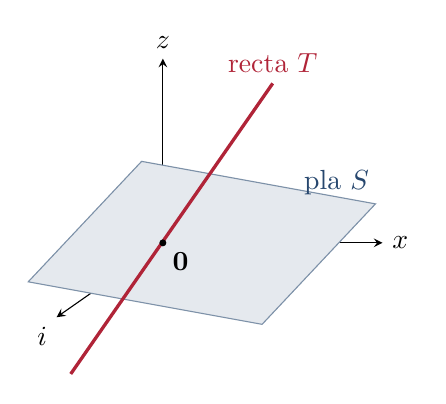
\begin{tikzpicture}[scale=0.9,>=stealth]
% Eixos en projecció obliqua
\draw[->] (0,0) -- (3.1,0) node[right]{$x$};
\draw[->] (0,0) -- (0,2.6) node[above]{$z$};
\draw[->] (0,0) -- (-1.5,-1.05) node[below left]{$i$};
% Pla per l'origen
\fill[figB!12,draw=figB!60] (-1.9,-0.55) -- (1.4,-1.15) -- (3.0,0.55) -- (-0.3,1.15) -- cycle;
\node[figB] at (2.45,0.85) {pla $S$};
% Recta per l'origen
\draw[very thick,figA] (-1.3,-1.85) -- (1.55,2.25) node[above]{recta $T$};
\fill (0,0) circle (1.4pt) node[below right]{$\mathbf{0}$};
\end{tikzpicture}

{\small\itshape A l'espai ordinari, els subespais propis no trivials són les rectes i els plans que passen per l'origen.}
\end{center}

\begin{observacio}
Fem les observacions següents:

\begin{enumerate}
\item Tot espai vectorial $E$ té almenys dos subespais. El
propi $E$ és un subespai i el conjunt $\left\{ \mathbf{0}%
\right\} $ és altre subespai anomenat subespai zero; respecte de la
inclusió de conjunts, podem afirmar que el primer és el més gran de
tots els subespais de $E$, i el més petit, és el segon. Tot
subespai diferent d'aquests dos s’anomena subespai vectorial \textbf{propi}
de $E$.

\item Distingirem la estructura d’espai vectorial d’un subconjunt $S$
que és subespai vectorial de $E$ per $S$.
\end{enumerate}
\end{observacio}

\begin{exemple}
En l’espai vectorial real $E$ dels vectors d'origen $O$ de l'
espai ordinari, es té dues classes de subespais vectorials (a banda
de $\left\{ \mathbf{0}\right\} $ i del propi $E$): (a) el conjunt
dels vectors d'origen $O$ situats sobre una recta que passa per $O$, i
(b) el conjunt dels vectors d'origen $O$ situats sobre un pla que
passa per $O$. Observeu que no hi ha cap altre subespai vectorial
de $E$ més que els que acabem de descriure.
\end{exemple}

\begin{exemple}
El conjunt dels nombres reals $\mathbb{R}$ és un subespai
vectorial de $\mathbb{C}$ considerat com a espai vectorial real.
\end{exemple}

\begin{exemple}
Demostreu que el conjunt $S$ de les matrius quadrades d’ordre 2 que
tenen zeros en la diagonal principal és un subespai de l’espai vectorial
real de totes les matrius quadrades d’ordre 2 amb coeficients reals.

\end{exemple}
\begin{solucio}
És clar que $S\neq \emptyset $. Siguin 
\begin{equation*}
A=\left( 
\begin{array}{cc}
0 & a_{12} \\ 
a_{21} & 0%
\end{array}%
\right) \text{ \ \ \ i \ \ \ }B=\left( 
\begin{array}{cc}
0 & b_{12} \\ 
b_{21} & 0%
\end{array}%
\right)
\end{equation*}%
dues matrius qualssevol de $S$ i $\lambda $ un escalar qualsevol. Aleshores%
\begin{equation*}
A+B=\left( 
\begin{array}{cc}
0 & a_{12}+b_{12} \\ 
a_{21}+b_{21} & 0%
\end{array}%
\right)
\end{equation*}%
i%
\begin{equation*}
\lambda A=\left( 
\begin{array}{cc}
0 & \lambda a_{12} \\ 
\lambda a_{21} & 0%
\end{array}%
\right)
\end{equation*}%
Debido a que $A+B$ i $\lambda A$ tenen zeros en la diagonal principal, están en $S$. Per consegüent, $S$ és un subespai vectorial.
\end{solucio}

\begin{exemple}
Sigui $n$ un nombre natural i suposem que $S$ consta de la funció
constant igual $0$ i de totes les funcions polinòmiques de grau com a
sumo $n$; és a dir, totes les funcions reals de variable real expressables
en la forma%
\begin{equation*}
p(x)=a_{0}+a_{1}x+\cdots +a_{n}x^{n}
\end{equation*}%
on $a_{0},a_{1},...,a_{n}$ són nombres reals. Demostreu que $S$
és un subespai de l’espai vectorial real de totes les funcions reals de
variable real.

\end{exemple}
\begin{solucio}
És clar que $S\neq \emptyset $. Siguin 
\begin{equation*}
p(x)=a_{0}+a_{1}x+\cdots +a_{n}x^{n}
\end{equation*}%
i%
\begin{equation*}
q(x)=b_{0}+b_{1}x+\cdots +b_{n}x^{n}
\end{equation*}%
Aleshores,%
\begin{align*}
(p+q)(x) &=p(x)+q(x)= \\
&=(a_{0}+b_{0})+(a_{1}+b_{1})x+\cdots +(a_{n}+b_{n})x^{n}
\end{align*}%
i%
\begin{align*}
(\lambda p)(x) &=\lambda p(x)= \\
&=(\lambda a_{0})+(\lambda a_{1})x+\cdots +(\lambda a_{n})x^{n}
\end{align*}%
tenen la forma adequada per afirmar que $p+q$ i $\lambda p$ estan en $%
S $. Per consegüent, $S$ és un subespai vectorial.
\end{solucio}

\begin{exemple}
Recordeu que si $f$ i $g$ són funcions contínues i $\lambda $ és una
constant real, aleshores $f+g$ i $\lambda f$ són funcions contínues. Se
concluye, doncs, que el conjunt de totes les funcions contínues és un
subespai de l’espai vectorial real de totes les funcions reals de
variable real.
\end{exemple}

\begin{exemple}
Considerem un sistema lineal de $m$ equacions amb $n$ incògnites:%
\begin{equation*}
\left. 
\begin{array}{ccccccccc}
a_{11}x_{1} & + & a_{12}x_{2} & + & \cdots & + & a_{1n}x_{n} & = & b_{1} \\ 
a_{21}x_{1} & + & a_{22}x_{2} & + & \cdots & + & a_{2n}x_{n} & = & b_{2} \\ 
\vdots &  & \vdots &  &  &  & \vdots &  & \vdots \\ 
a_{m1}x_{1} & + & a_{m2}x_{2} & + & \cdots & + & a_{mn}x_{n} & = & b_{m}%
\end{array}%
\right\}
\end{equation*}%
o bé, en notació matricial, $A\mathbf{x}=\mathbf{b}$, essent%
\begin{equation*}
A=\left( 
\begin{array}{cccc}
a_{11} & a_{12} & \cdots & a_{1n} \\ 
a_{21} & a_{22} & \cdots & a_{2n} \\ 
\vdots & \vdots & \ddots & \vdots \\ 
a_{m1} & a_{m2} & \cdots & a_{mn}%
\end{array}%
\right)
\end{equation*}%
i%
\begin{equation*}
\mathbf{x}=\left( 
\begin{array}{c}
x_{1} \\ 
x_{2} \\ 
\vdots \\ 
x_{n}%
\end{array}%
\right) \text{ \ \ \ i \ \ \ }\mathbf{b}=\left( 
\begin{array}{c}
b_{1} \\ 
b_{2} \\ 
\vdots \\ 
b_{m}%
\end{array}%
\right)
\end{equation*}%
Es diu que un vector columna de $\mathbb{R}^{n}$ 
\begin{equation*}
\mathbf{s}=\left( 
\begin{array}{c}
s_{1} \\ 
s_{2} \\ 
\vdots \\ 
s_{n}%
\end{array}%
\right)
\end{equation*}%
és un vector solució del sistema si $%
x_{1}=s_{1},x_{2}=s_{2},...,x_{n}=s_{n}$ és una solució de tal sistema.
Demostreu que el conjunt de vectors solució d’un sistema homogeni és un subespai de $\mathbb{R}^{n}$. Un sistema lineal s’anomena homogeni si tots els seus termes independents són nuls, és a dir, $%
b_{1}=\cdots =b_{m}=0$.

\end{exemple}
\begin{solucio}
Sigui $A\mathbf{x}=\mathbf{0}$ un sistema lineal homogeni de $m$
equacions amb $n$ incògnites, $S$ el conjunt de vectors solució,
i $\mathbf{s}$ i $\mathbf{t}$ vectors de $S$. Com que $\mathbf{s}$ i $%
\mathbf{t}$ són vectors solució del sistema, es té%
\begin{equation*}
A\mathbf{s}=\mathbf{0}\text{ \ \ \ i \ \ \ }A\mathbf{t}=\mathbf{0}
\end{equation*}%
Per tant,%
\begin{equation*}
A(\mathbf{s}+\mathbf{t})=A\mathbf{s}+A\mathbf{t}=\mathbf{0}+\mathbf{0}=%
\mathbf{0}
\end{equation*}%
i%
\begin{equation*}
A\left( \lambda \mathbf{s}\right) =\lambda \left( A\mathbf{s}\right)
=\lambda \mathbf{0}=\mathbf{0}
\end{equation*}%
De on, $\mathbf{s}+\mathbf{t}$ i $\lambda \mathbf{s}$
satisfan l’equació $A\mathbf{x}=\mathbf{0}$. Per tant, $\mathbf{s}+%
\mathbf{t}$ i $\lambda \mathbf{s}$ són vectors solució i, en
conseqüència, $S$ és un subespai vectorial que és habitual denominarlo
subespai solució del sistema $A\mathbf{x}=\mathbf{0}$.
\end{solucio}

\section{Intersecció de subespais vectorials}

\begin{teorema}
La intersecció $S\cap T$ de dos subespais
qualssevol $S$ i $T$ d’un espai vectorial $E$
és també un subespai de $E$.

\end{teorema}
\begin{prova}
La intersecció $S\cap T$ es defineix com el conjunt de tots els
elements que pertanyen simultàniament a $S$ i $T$. Si $\mathbf{u},%
\mathbf{v}\in S\cap T$, aleshores $\mathbf{u},\mathbf{v}\in 
S$ i $\mathbf{u},\mathbf{v}\in T$. Com que tots dos són
subespais, es té $\mathbf{u}+\mathbf{v}\in S$ i $\mathbf{u}+%
\mathbf{v}\in T$ i per tant $\mathbf{u}+\mathbf{v}\in S%
\cap T$. Anàlogament, tot múltiple escalar $\lambda 
\mathbf{u}$ aquestará en $S\cap T$ sempre que hi estigui
$\mathbf{u}$.
\end{prova}

\begin{observacio}
Fem les observacions següents:

\begin{enumerate}
\item Donats dos subespais $S$ i $T$ de $E$, $%
S\cap T$ és el subespai més gran contingut en tots dos.

\item En general, si $\mathcal{F}$ és una família qualsevol de subespais
vectorials de $E$, es demostra de la mateixa manera que 
\begin{equation*}
\bigcap_{F\in \mathcal{F}}F
\end{equation*}%
és també un subespai vectorial de $E$.
\end{enumerate}
\end{observacio}

\begin{exemple}
Determineu la intersecció dels subespais vectorials 
\begin{align*}
S &=\left\{ (x,y,z)\in \mathbb{R}^{3}:x-2y+z=0\right\} \\
T &=\left\{ (x,y,z)\in \mathbb{R}^{3}:x=0\right\}
\end{align*}
de $\mathbb{R}^{3}$.

\end{exemple}
\begin{solucio}
Observeu que $S$ i $T$ són subespais vectorials de 
$\mathbb{R}^{3}$ perquè tots dos estan definits per equacions lineals
homogènies. Qualsevol vector de $S$ és solució de l'equació lineal 
\begin{equation*}
x-2y+z=0
\end{equation*}%
De la mateixa manera, qualsevol vector de $T$ és solució de l'equació lineal%
\begin{equation*}
x=0
\end{equation*}%
Aleshores, qualsevol vector $(x,y,z)\in S\cap T$ ha de ser
solució del sistema%
\begin{equation*}
\left. 
\begin{array}{r}
x-2y+z=0 \\ 
x=0%
\end{array}%
\right\}
\end{equation*}%
és a dir,%
\begin{equation*}
S\cap T=\left\{ (x,y,z)\in \mathbb{R}^{3}:-2y+z=0\text{ i }%
x=0\right\}
\end{equation*}
\end{solucio}

\section{Subespai generat per un subconjunt}

\begin{definicio}
Donat un subconjunt no buit $A$ de $E$, s’anomena \textbf{%
subespai generat} per $A$ al més petit dels subespais vectorials de $%
E$ que contenen $A$. Denotem per $\left\langle A\right\rangle $
el subespai generat per $A$.
\end{definicio}

\begin{observacio}
Fem les observacions següents:

\begin{enumerate}
\item Dit d'una altra manera, $\left\langle A\right\rangle $ és el subconjunt
de $E$ que compleix:

\begin{enumerate}
\item $\left\langle A\right\rangle $ és un subespai vectorial de $E$

\item $A\subset \left\langle A\right\rangle $

\item Si $S$ és un subespai vectorial de $E$ tal que $%
A\subset S$, aleshores ha de complirse que $\left\langle
A\right\rangle \subset S$.
\end{enumerate}

\item És evident que si $S$ és un subespai vectorial de $E$, aleshores el subespai generat per $S$ és el mateix $S$.
\end{enumerate}
\end{observacio}

\begin{teorema}
Donat un subconjunt no buit $A$ de $E$, es compleix%
\begin{equation*}
\left\langle A\right\rangle =\bigcap_{F\in \mathcal{F}}F
\end{equation*}%
on $\mathcal{F}$ és la família (no buida, ja que $E$
pertany a la família) de tots els subespais vectorials de $E$
contenen $A$.

\end{teorema}
\begin{prova}
En efecte, si $\mathcal{F}$ és la família de tots els subespais de $%
E$ que contenen $A$, aleshores és clar que 
\begin{equation*}
\bigcap_{F\in \mathcal{F}}F
\end{equation*}%
verifica les tres condicions indicades en la darrera observació.
\end{prova}

\begin{exemple}
Demostreu que si $\mathbf{v}$ és un vector de $E$ i $A=\left\{ 
\mathbf{v}\right\} $, aleshores $\left\langle A\right\rangle =\left\{ \lambda 
\mathbf{v}:\lambda \in \mathbb{K}\right\} $.

\end{exemple}
\begin{solucio}
El conjunt $\left\{ \lambda \mathbf{v}:\lambda \in \mathbb{K}\right\} $ és
un subespai de $E$, ja que%
\begin{equation*}
(\lambda \mathbf{v})+(\mu \mathbf{v})=(\lambda +\mu )\mathbf{v}
\end{equation*}%
i%
\begin{equation*}
\mu (\lambda \mathbf{v})=(\mu \lambda )\mathbf{v}
\end{equation*}%
A més, $\mathbf{v}$ és en aquest conjunt, ja que%
\begin{equation*}
\mathbf{v}=1\mathbf{v}
\end{equation*}%
Finalment, és el subespai més petit que conté $A$ per construcció.
\end{solucio}

\section{Suma de subespais vectorials}

\begin{definicio}
Donats dos subespais vectorials $S$ i $T$ de $E$%
, s’anomena subespai \textbf{suma} de $S$ i $T$ denotat
per $S+T$ el subespai vectorial generat pel
conjunt $S\cup T$. En símbols%
\begin{equation*}
S+T=\left\langle S\cup T\right\rangle
\end{equation*}
\end{definicio}

\begin{teorema}
Donats dos subespais vectorials $S$ i $T$ de $E$%
, aleshores el subespai suma compleix%
\begin{equation*}
S+T=\left\{ \mathbf{s}+\mathbf{t}:\mathbf{s}\in S,%
\mathbf{t}\in T\right\}
\end{equation*}

\end{teorema}
\begin{prova}
En efecte, si prenem dos elements qualssevol d’aquesta forma $\mathbf{s}%
_{1}+\mathbf{t}_{1}$ i $\mathbf{s}_{2}+\mathbf{t}_{2}$, aleshores es té 
\begin{equation*}
(\mathbf{s}_{1}+\mathbf{t}_{1})+(\mathbf{s}_{2}+\mathbf{t}_{2})=\mathbf{s}%
_{1}+(\mathbf{t}_{1}+\mathbf{s}_{2})+\mathbf{t}_{2}=(\mathbf{s}_{1}+\mathbf{s%
}_{2})+(\mathbf{t}_{1}+\mathbf{t}_{2})
\end{equation*}%
que és un altre element de la mateixa forma. A més, també tenim 
\begin{equation*}
\lambda (\mathbf{s}+\mathbf{t})=\lambda \mathbf{s}+\lambda \mathbf{t}
\end{equation*}%
Per tant, el conjunt $\left\{ \mathbf{s}+\mathbf{t}:\mathbf{s}\in S,\mathbf{t}\in T\right\} $ és un subespai de $E$. Per
d’altra banda, de la manera com s'ha definit és clar que és el més petit
subespai que conté $S$ i $T$, i en conseqüència
tenim el que volíem demostrar.
\end{prova}

\begin{observacio}
Fem les observacions importants següents:

\begin{enumerate}
\item En general, $S\cup T$ no és un subespai vectorial de $E$.
Per provar-ho, considerem els subespais vectorials $S=\left\{
(x,0):x\in \mathbb{R}\right\} $ i $T=\left\{ (0,y):y\in \mathbb{R}%
\right\} $ de $\mathbb{R}^{2}$. La suma $(1,0)+(0,1)=(1,1)$ no pertany a $%
S$ ni a $T$.

\item Donats dos subespais $S$ i $T$ de $E$, $%
S+T$ és el subespai més petit que conté tots dos.
\end{enumerate}
\end{observacio}

\begin{observacio}
Un vector $\mathbf{v}$ de $S+T$ pot, en general,
descompondre's de diverses maneras en la forma $\mathbf{s}+\mathbf{t}$. Si%
\begin{equation*}
\mathbf{v}=\mathbf{s}_{1}+\mathbf{t}_{1}=\mathbf{s}_{2}+\mathbf{t}_{2}
\end{equation*}%
aleshores%
\begin{equation*}
\mathbf{w}=\mathbf{s}_{1}-\mathbf{s}_{2}=\mathbf{t}_{2}-\mathbf{t}_{1}
\end{equation*}%
i el vector $\mathbf{w}$ obtingut d’aquesta forma, que pertany a $S$
i $T$, també pertany a la seva intersecció. Recíprocament, qualsevol que sigui $\mathbf{w}\in S\cap T$, es
té%
\begin{equation*}
\mathbf{v}=\mathbf{s}+\mathbf{t}=(\mathbf{s}+\mathbf{x})+(\mathbf{t}-\mathbf{%
x})
\end{equation*}%
Aquesta observació justifica la proposició i definició
següents.
\end{observacio}

\begin{teorema}
Donats dos subespais vectorials $S$ i $T$ d’un espai
vectorial $E$, aleshores les tres condicions següents són
equivalents:

\begin{enumerate}
\item La descomposició de tot vector $\mathbf{v}$ de $S+%
T$ en suma d’un vector $\mathbf{s}$ de $S$ i d’un vector 
$\mathbf{t}$ de $T$ és única

\item Si $\mathbf{s}+\mathbf{t}=\mathbf{0}$, amb $\mathbf{s}\in S$
i $\mathbf{t}\in T$, es compleix que $\mathbf{s}=\mathbf{t}=\mathbf{0}
$

\item $S\cap T=\left\{ \mathbf{0}\right\} $
\end{enumerate}

\end{teorema}
\begin{prova}
(1) implica (2). Donat que podem escriure%
\begin{equation*}
\mathbf{s}+\mathbf{t}=\mathbf{0}+\mathbf{0}
\end{equation*}%
es dedueix $\mathbf{s}=\mathbf{t}=\mathbf{0}$.

(2) implica (3). Suposem que $\mathbf{v}\in S\cap T$,
podem escriure%
\begin{equation*}
\mathbf{0}=\mathbf{v}+(-\mathbf{v})
\end{equation*}%
on $\mathbf{v}\in S$ i $-\mathbf{v}\in T$. De (2) es
dedueix $\mathbf{v}=\mathbf{0}$.

(3) implica (1). Suposem que tenim un vector $\mathbf{v}$ de $S%
+T$ expressat de dues maneres%
\begin{equation*}
\mathbf{v}=\mathbf{s}_{1}+\mathbf{t}_{1}=\mathbf{s}_{2}+\mathbf{t}_{2}
\end{equation*}%
aleshores%
\begin{equation*}
\mathbf{s}_{1}-\mathbf{s}_{2}=\mathbf{t}_{2}-\mathbf{t}_{1}=0
\end{equation*}%
ja que $\mathbf{s}_{1}-\mathbf{s}_{2}=\mathbf{t}_{2}-\mathbf{t}_{1}$ és un
vector de $S\cap T$ que per hipòtesi ha de ser $%
\mathbf{0}$.
\end{prova}

\begin{definicio}
Donats dos subespais vectorials $S$ i $T$ d’un espai
vectorial $E$. Si $S\cap T=\left\{ \mathbf{0}%
\right\} $, aleshores es diu que la suma de subespais $S+T$ és una \textbf{suma directa} i la designem amb la notació%
\begin{equation*}
S\oplus T
\end{equation*}
\end{definicio}

\begin{center}
\definecolor{figA}{HTML}{B02438}\definecolor{figB}{HTML}{27476E}%
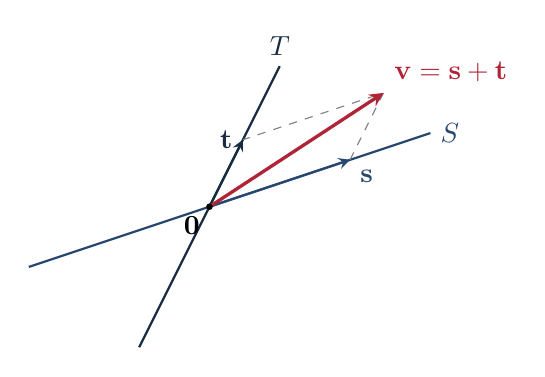
\begin{tikzpicture}[scale=0.85,>=stealth]
\draw[thick,figB] (-2.7,-0.9) -- (3.3,1.1) node[right]{$S$};
\draw[thick,figB!60!black] (-1.05,-2.1) -- (1.05,2.1) node[above]{$T$};
\coordinate (s) at (2.1,0.7);
\coordinate (tt) at (0.5,1.0);
\coordinate (v) at (2.6,1.7);
\draw[dashed,gray] (s) -- (v) -- (tt);
\draw[->,thick,figB] (0,0) -- (s) node[below right]{$\mathbf{s}$};
\draw[->,thick,figB!60!black] (0,0) -- (tt) node[left]{$\mathbf{t}$};
\draw[->,very thick,figA] (0,0) -- (v) node[above right]{$\mathbf{v}=\mathbf{s}+\mathbf{t}$};
\fill (0,0) circle (1.4pt) node[below left]{$\mathbf{0}$};
\end{tikzpicture}

{\small\itshape Si $S\cap T=\{\mathbf{0}\}$, cada vector de la suma és descompon de manera única: $\mathbf{v}=\mathbf{s}+\mathbf{t}$.}
\end{center}

\begin{observacio}
Fem les observacions següents:

\begin{enumerate}
\item De vegades es diu que dos subespais $S$ i $T$ d’un
espai vectorial $E$ són \textbf{independents} quan $S%
\cap T=\left\{ \mathbf{0}\right\} $. En aquest cas, la seva suma és
directa.

\item En general, si $S_{1},...,S_{m}$ és una família
finita de subespais de $E$, la seva suma es defineix com segueix%
\begin{equation*}
\sum_{i=1}^{n}S_{i}=S_{1}+\cdots +S_{m}=\left\{
\sum_{i=1}^{m}\mathbf{v}_{i}:\mathbf{v}_{i}\in S_{i}\right\}
\end{equation*}%
que és un subespai de $E$. La suma és directa, i es denota
per 
\begin{equation*}
\bigoplus_{i=1}^{n}S_{i}=S_{1}\oplus \cdots \oplus S_{m}
\end{equation*}%
si la descomposició d’un vector d’aquest subespai només és possible
d’una manera. Per fer-ho és necessari i suficient que la igualtat%
\begin{equation*}
\sum_{i=1}^{m}\mathbf{v}_{i}=0
\end{equation*}%
es verifiqui únicament escollint tots els vectors $\mathbf{v}_{i}$
nuls.
\end{enumerate}
\end{observacio}

\begin{definicio}
Es diu que $S_{1}$ i $S_{2}$ són dos \textbf{subespais
suplementaris} de $E$ si tot vector $\mathbf{v}$ de $E$
pot escriure’s de manera única en la forma%
\begin{equation*}
\mathbf{v}=\mathbf{v}_{1}+\mathbf{v}_{2}
\end{equation*}%
on $\mathbf{v}_{1}\in S_{1}$ i $\mathbf{v}_{2}\in S%
_{2}$.
\end{definicio}

\begin{corollari}
Dos subespais vectorials $S_{1}$ i $S_{2}$ de $E$ són suplementaris si i només si%
\begin{equation*}
E=S_{1}\oplus S_{2}
\end{equation*}
\end{corollari}

\begin{observacio}
Fem les observacions importants següents:

\begin{enumerate}
\item Quan es compleix%
\begin{equation*}
E=S_{1}\oplus S_{2}
\end{equation*}%
En tal cas es diu que $S_{1}$(resp. $S_{2}$) és un
suplementari de $S_{2}$ (resp. $S_{1}$) respecte de $%
E$. En tal cas, qualsevol vector $\mathbf{v}$ de $E$
pot escriure’s de manera única en la forma%
\begin{equation*}
\mathbf{v}=\mathbf{v}_{1}+\mathbf{v}_{2}
\end{equation*}%
on $\mathbf{v}_{1}\in S_{1}$ i $\mathbf{v}_{2}\in S%
_{2}$.

\item És natural plantejar-se dues preguntes: si $S_{1}$ és un
subespai de $E$, existeix un suplementari $%
S_{2}$ de $S_{1}$ respecte de $E$, i, si existeix,
és únic? La resposta a la segona pregunta és negativa, segons el 
\textbf{teorema 21}, però més endavant tenim el \textbf{corol·lari 9}.
Respecte de la primera, la resposta és afirmativa segons el mateix teorema.

\item No s’ha de confondre un suplementari del subespai $S$
respecte de $E$ amb el complementari del conjunt $S$ respecte de $%
E$. En aquest darrer cas, no és un subespai de $E$ ja
que no conté el $\mathbf{0}$.
\end{enumerate}
\end{observacio}

\begin{exemple}
En $\mathbb{R}^{3}$ es consideren els subespais $S$ i $T$
generats pels conjunts $\{(2,3,0),(3,1,2)\}$ i $\{(1,-2,2)\}$
respectivament. Determineu el subespai $S+T$ i
averiguar si és suma directa.

\end{exemple}
\begin{solucio}
Segons el teorema, un vector $(x,y,z)$ de $S+T$ és de la forma%
\begin{equation*}
(x,y,z)=\lambda (2,3,0)+\mu (3,1,2)+\delta (1,-2,2)
\end{equation*}%
Efectuant operacions, s’obté%
\begin{equation*}
(x,y,z)=(2\lambda +3\mu +\delta ,3\lambda +\mu -2\delta ,2\mu +2\delta )
\end{equation*}%
Igualant components, es té%
\begin{equation*}
\left. 
\begin{array}{ll}
E_{1}: & x=2\lambda +3\mu +\delta \\ 
E_{2}: & i=3\lambda +\mu -2\delta \\ 
E_{3}: & z=2\mu +2\delta%
\end{array}%
\right\}
\end{equation*}%
D’aquí s’obté%
\begin{equation*}
\left. 
\begin{array}{rr}
3E_{1}-2E_{2}: & 3x-2y=7\mu +7\delta \\ 
E_{3}: & z=2\mu +2\delta%
\end{array}%
\right\}
\end{equation*}%
D’aquí s’obté%
\begin{equation*}
\begin{array}{cc}
2(3E_{1}-2E_{2})-7E_{3}: & 6x-4y-7z=0%
\end{array}%
\end{equation*}%
Per consegüent%
\begin{equation*}
S+T=\{(x,y,z)\in R^{3}:6x-4y-7z=0\}
\end{equation*}%
Per saber si la suma és directa hem d’esbrinar si els subespais són o
no independents. Per fer-ho, hem de calculeu $S\cap T$. Un vector $(x,y,z)$
de $S\cap T$ ha de complir%
\begin{equation*}
(x,y,z)=\alpha (2,3,0)+\beta (3,1,2)
\end{equation*}%
i%
\begin{equation*}
(x,y,z)=\gamma (1,-2,2)
\end{equation*}%
Per tant,%
\begin{equation*}
\alpha (2,3,0)+\beta (3,1,2)=\gamma (1,-2,2)
\end{equation*}%
és a dir%
\begin{equation*}
(2\alpha +3\beta ,3\alpha +\beta ,2\beta )=(\gamma ,-2\gamma ,2\gamma )
\end{equation*}%
d’on s’obté%
\begin{equation*}
\left. 
\begin{array}{r}
2\alpha +3\beta =\gamma \\ 
3\alpha +\beta =-2\gamma \\ 
2\beta =2\gamma%
\end{array}%
\right\}
\end{equation*}%
Tenim $\beta =\gamma $. Per tant, $\alpha =-\beta =-\gamma $. Prenent $%
\gamma =1$, s’obté%
\begin{equation*}
(1,-2,2)=-(2,3,0)+(3,1,2)
\end{equation*}%
el que significa que%
\begin{equation*}
(1,-2,2)\in S\cap T
\end{equation*}%
Per consegüent,%
\begin{equation*}
S\cap T\neq \{0\}
\end{equation*}%
i la suma no és directa.
\end{solucio}

\section{Combinacions lineals}

\begin{definicio}
S’anomena \textbf{sistema} de vectors de $E$ a qualsevol successió finita $\mathcal{S}$ de vectors de $E$. D’aquesta manera, $\mathcal{S%
}=(\mathbf{v}_{1},\mathbf{v}_{2},...,\mathbf{v}_{m})$, amb $\mathbf{v}%
_{i}\in E$ ($i=1,...,m$), és un sistema de vectors de $E$.
\end{definicio}

\begin{observacio}
Cal anar amb compte de no confondre el sistema de vectors $(\mathbf{v}%
_{1},\mathbf{v}_{2},...,\mathbf{v}_{m})$ amb el conjunt $\left\{ \mathbf{v}%
_{1},\mathbf{v}_{2},...,\mathbf{v}_{m}\right\} $ els elements del qual són els
vectors del sistema. Per exemple, el sistema $(1,1,1)$ de vectors de $%
\mathbb{R}$ té com conjunt de vectors $\left\{ 1\right\} $; i els
sistemes diferents $(1,2,3)$ i $(2,1,3)$ de $\mathbb{R}$ tenen el mateix
conjunt de vectors $\left\{ 1,2,3\right\} $.

Quan escriguem ``sistema de vectors'' ens referirem a la successió
finita de vectors. En canvi, quan escriguem ``vectors del sistema''
ens referirem al conjunt dels vectors de la successió.
\end{observacio}

\begin{definicio}
Donat un sistema $\mathcal{S}=(\mathbf{v}_{1},\mathbf{v}_{2},...,\mathbf{v}%
_{m})$ de vectors de $E$. Es diu que un vector $\mathbf{v}$ de $%
E$ és \textbf{combinació lineal} dels vectors del sistema $%
\mathcal{S}$ si existeix una successió finita $(\lambda _{1},\lambda
_{2},...,\lambda _{m})$ d’elements de $\mathbb{K}$ tals que%
\begin{equation*}
\mathbf{v}=\lambda _{1}\mathbf{v}_{1}+\lambda _{2}\mathbf{v}_{2}+\cdots
+\lambda _{m}\mathbf{v}_{m}
\end{equation*}%
Els escalars $\lambda _{i}$ ($i=1,...,m$) s’anomenan \textbf{coeficients}
de la combinació lineal.

També es diu aleshores que el vector $\mathbf{v}$ \textbf{depèn
linealment} dels vectors del sistema $\mathcal{S}$.

\end{definicio}
\begin{observacio}
Més en general, si $\mathcal{S}=(\mathbf{v}_{i})_{i\in I}$ és una
família qualsevol (finita o no) de vectors de $E$, es diu que un
vector $\mathbf{v}$ de $E$ és combinació lineal dels
vectors de la família $\mathcal{S}$ si existeix una família $(\lambda
_{i})_{i\in I}$ d’elements de $\mathbb{K}$ tals que només un nombre \textbf{finit} dels escalars $\lambda _{i}$ són no nuls i 
\begin{equation*}
\mathbf{v}=\sum_{i\in I}\lambda _{i}\mathbf{v}_{i}
\end{equation*}

Observeu que si $J\subset I$, $J$ és finit i tal que $\lambda _{i}=0$
per a tot $i\in I-J$, aleshores%
\begin{equation*}
\sum_{i\in I}\lambda _{i}\mathbf{v}_{i}=\sum_{i\in J}\lambda _{i}\mathbf{v}%
_{i}
\end{equation*}%
És evident que el valor del segon membre de la igualtat anterior no
depèn de $J$ (sempre que $J$ satisfaci les condicions enunciades). Com a
conseqüència, tenim que un vector $\mathbf{v}$ de $E$ és combinació lineal dels vectors de la família $(\mathbf{v}_{i})_{i\in I}$ si
ho és d’una \textbf{subfamília finita} de $(\mathbf{v}_{i})_{i\in I}$.
\end{observacio}

\begin{teorema}
Es dedueixen immediatament de la definició els següents resultats:

\begin{enumerate}
\item El vector $\mathbf{0}$ és combinació lineal dels vectors de
qualsevol sistema.

\item Tot vector és combinació lineal dels vectors de qualsevol
sistema que lo conté.

\item Si $\mathbf{v}$ és combinació lineal dels vectors del sistema $%
(\mathbf{v}_{1},\mathbf{v}_{2},...,\mathbf{v}_{m})$ i si cada $\mathbf{v}%
_{i} $ ($i=1,2,...,m$) és combinació lineal dels vectors del sistema 
$(\mathbf{w}_{1},\mathbf{w}_{2},...,\mathbf{w}_{p})$, el vector $\mathbf{v}$
és combinació lineal de dels vectors del sistema $(\mathbf{w}_{1},%
\mathbf{w}_{2},...,\mathbf{w}_{p})$.
\end{enumerate}

\end{teorema}
\begin{prova}
(1.) És suficient triar tots els coeficients nuls.

(2.) En efecte,%
\begin{equation*}
\mathbf{v}=1\mathbf{v}
\end{equation*}%
i, si hi ha altres vectors, els assignem a tots coeficient nul.

(3.) Si%
\begin{equation*}
\mathbf{v}_{i}=\sum_{j=1}^{p}\mu _{ij}\mathbf{w}_{j}
\end{equation*}%
i%
\begin{equation*}
\mathbf{v}=\lambda _{1}\mathbf{v}_{1}+\lambda _{2}\mathbf{v}_{2}+\cdots
+\lambda _{m}\mathbf{v}_{m}
\end{equation*}%
aleshores, per substitució i per les regles de càlcul, tenim%
\begin{align*}
\mathbf{v} &=\lambda _{1}\left( \sum_{j=1}^{p}\mu _{1j}\mathbf{w}%
_{j}\right) +\lambda _{2}\left( \sum_{j=1}^{p}\mu _{2j}\mathbf{w}_{j}\right)
+\cdots +\lambda _{m}\left( \sum_{j=1}^{p}\mu _{mj}\mathbf{w}_{j}\right) \\
&=\left( \sum_{k=1}^{m}\lambda _{k}\mu _{k1}\right) \mathbf{w}_{1}+\left(
\sum_{k=1}^{m}\lambda _{k}\mu _{k2}\right) \mathbf{w}_{2}+\cdots +\left(
\sum_{k=1}^{m}\lambda _{k}\mu _{kp}\right) \mathbf{w}_{p}
\end{align*}
\end{prova}

\begin{observacio}
Aquest darrer resultat s’expressa també així: si $\mathbf{v}$
depèn linealment dels vectors $\mathbf{v}_{1},\mathbf{v}_{2},...,%
\mathbf{v}_{m}$, i cadascun d’aquests depèn linealment de $\mathbf{w}_{1},%
\mathbf{w}_{2},...,\mathbf{w}_{p}$, el vector $\mathbf{v}$ depèn
linealment d’aquests darrers. Per aquesta raó, aquest resultat es le
conoce com propietat transitiva de la dependència lineal.
\end{observacio}

\begin{exemple}
Considerem els vectors $\mathbf{u}=(1,2,-1)$ i $\mathbf{v}=(6,4,2)$ de $%
\mathbb{R}^{3}$. Demostreu que $\mathbf{w}=(9,2,7)$ és combinació
lineal de $\mathbf{u}$ i $\mathbf{v}$, i que, en canvi, $\mathbf{w}^{\prime
}=(4,-1,8)$ no és combinació lineal de $\mathbf{u}$ i $\mathbf{v}$.

\end{exemple}
\begin{solucio}
Perquè $\mathbf{w}$ sigui una combinació lineal de $\mathbf{u}$ i $%
\mathbf{v}$, han de existir els escalars $\lambda _{1}$ i $\lambda _{2}$
tals que $\mathbf{w}=\lambda _{1}\mathbf{u}+\lambda _{2}\mathbf{v}$, és
dir,%
\begin{equation*}
(9,2,7)=\lambda _{1}(1,2,-1)+\lambda _{2}(6,4,2)
\end{equation*}%
o bé,%
\begin{equation*}
(9,2,7)=(\lambda _{1}+6\lambda _{2},2\lambda _{1}+4\lambda _{2},-\lambda
_{1}+2\lambda _{2})
\end{equation*}%
Al igualar les components corresponents, s’obté el sistema següent%
\begin{equation*}
\left. 
\begin{array}{r}
\lambda _{1}+6\lambda _{2}=9 \\ 
2\lambda _{1}+4\lambda _{2}=2 \\ 
-\lambda _{1}+2\lambda _{2}=7%
\end{array}%
\right\}
\end{equation*}%
Si es resol aquest sistema, s’obté la solució $\lambda _{1}=-3$ i $%
\lambda _{2}=2$. D’aquesta manera, tenim%
\begin{equation*}
\mathbf{w}=-3\mathbf{u}+2\mathbf{v}
\end{equation*}

De la mateixa manera, perquè $\mathbf{w}^{\prime }$ sigui una combinació
lineal de $\mathbf{u}$ i $\mathbf{v}$ han de existir $\lambda _{1}$ i $%
\lambda _{2}$ tals que%
\begin{equation*}
(4,-1,8)=\lambda _{1}(1,2,-1)+\lambda _{2}(6,4,2)
\end{equation*}%
o bé,%
\begin{equation*}
(4,-1,8)=(\lambda _{1}+6\lambda _{2},2\lambda _{1}+4\lambda _{2},-\lambda
_{1}+2\lambda _{2})
\end{equation*}%
Igualant components, s’obté%
\begin{equation*}
\left. 
\begin{array}{r}
\lambda _{1}+6\lambda _{2}=4 \\ 
2\lambda _{1}+4\lambda _{2}=-1 \\ 
-\lambda _{1}+2\lambda _{2}=8%
\end{array}%
\right\}
\end{equation*}%
Aquest sistema d'equacions és incompatible, de manera que no existeixen aquests
escalars. Com a conseqüència, $\mathbf{w}^{\prime }$ no és una combinació lineal de $\mathbf{u}$ i $\mathbf{v}$.
\end{solucio}

\section{Clausura lineal}

\begin{definicio}
S’anomena \textbf{clausura lineal} del sistema $\mathcal{S}=(\mathbf{v}_{1},%
\mathbf{v}_{2},...,\mathbf{v}_{m})$ al conjunt de tots els vectors de $%
E$ que són combinació lineal dels vectors de $\mathcal{S}$.
Denotem aquest conjunt per $\left\langle \mathbf{v}_{1},\mathbf{v}_{2},...,%
\mathbf{v}_{m}\right\rangle $.
\end{definicio}

\begin{center}
\definecolor{figA}{HTML}{B02438}\definecolor{figB}{HTML}{27476E}%
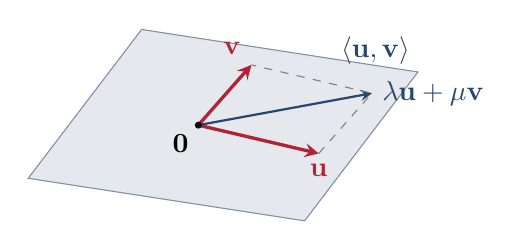
\begin{tikzpicture}[scale=0.9,>=stealth]
\fill[figB!12,draw=figB!60] (-2.4,-0.75) -- (1.5,-1.35) -- (3.1,0.75) -- (-0.8,1.35) -- cycle;
\node[figB] at (2.5,1.05) {$\left\langle \mathbf{u},\mathbf{v}\right\rangle $};
\draw[->,very thick,figA] (0,0) -- (1.7,-0.4) node[below]{$\mathbf{u}$};
\draw[->,very thick,figA] (0,0) -- (0.75,0.85) node[above left]{$\mathbf{v}$};
\draw[->,thick,figB] (0,0) -- (2.45,0.45) node[right]{$\lambda \mathbf{u}+\mu \mathbf{v}$};
\draw[dashed,gray] (1.7,-0.4) -- (2.45,0.45) -- (0.75,0.85);
\fill (0,0) circle (1.4pt) node[below left]{$\mathbf{0}$};
\end{tikzpicture}

{\small\itshape La clausura lineal de dos vectors no proporcionals de l'espai és el pla que determinen: el conjunt de totes les seves combinacions lineals.}
\end{center}

\begin{teorema}
La clausura lineal de qualsevol sistema és un subespai vectorial de $%
E$.

\end{teorema}
\begin{prova}
En efecte, de les relacions següents%
\begin{align*}
(\lambda _{1}\mathbf{v}_{1}+\cdots +\lambda _{m}\mathbf{v}_{m})+(\mu _{1}%
\mathbf{v}_{1}+\cdots +\mu _{m}\mathbf{v}_{m}) &=(\lambda _{1}+\mu _{1})%
\mathbf{v}_{1}+\cdots +(\lambda _{m}+\mu _{m})\mathbf{v}_{m} \\
\delta (\lambda _{1}\mathbf{v}_{1}+\cdots +\lambda _{m}\mathbf{v}_{m})
&=(\delta \lambda _{1})\mathbf{v}_{1}+\cdots +(\delta \lambda _{m})\mathbf{v%
}_{m}
\end{align*}%
es dedueix immediatament el que volem demostrar.
\end{prova}

\begin{definicio}
Un subespai vectorial $S$ de $E$ es diu que està 
\textbf{generat} pel sistema $\mathcal{S}=(\mathbf{v}_{1},\mathbf{v}%
_{2},...,\mathbf{v}_{m})$ si $S$ és la clausura lineal del sistema,
és a dir, si es compleix 
\begin{equation*}
S=\left\langle \mathbf{v}_{1},\mathbf{v}_{2},...,\mathbf{v}%
_{m}\right\rangle
\end{equation*}%
També es diu que $\mathcal{S}$ és un \textbf{sistema generador} del
subespai $S$.
\end{definicio}

\begin{teorema}
La clausura lineal d’un sistema és el subespai més petit vectorial que
conté al conjunt dels vectors del sistema.

\end{teorema}
\begin{prova}
Donat un sistema qualsevol $\mathcal{S}=(\mathbf{v}_{1},\mathbf{v}_{2},...,%
\mathbf{v}_{m})$. Sigui $A=\left\{ \mathbf{v}_{1},\mathbf{v}_{2},...,\mathbf{v}%
_{m}\right\} $ el conjunt dels vectors de $\mathcal{S}$. Pel teorema
anterior la clausura lineal és un subespai vectorial de $E$. Per a
qualsevol $\mathbf{v}_{i}\in A$ ($i=1,...,m$) es compleix%
\begin{equation*}
\mathbf{v}_{i}=0\mathbf{v}_{1}+\cdots +1\mathbf{v}_{i}+\cdots +0\mathbf{v}%
_{m}
\end{equation*}%
amb el que $A$ està contingut en la clausura lineal de $\mathcal{S}$. Si 
$S$ és qualsevol subespai de $E$ que conté $A$,
aleshores qualsevol combinació lineal dels vectors de $A$ és
clarament un altre vector de $S$. Per tant, la clausura lineal de\ $%
\mathcal{S}$ està contingut en $S$ i, en conseqüència, és el
més petit subespai vectorial que conté $A$.
\end{prova}

\begin{observacio}
Les nocions i propietats anteriors poden ampliar-se al cas d’una
família qualsevol $(\mathbf{v}_{i})_{i\in I}$, finita o no, de vectors de $%
E$. S’anomena clausura lineal d’una família $(\mathbf{v}_{i})_{i\in
I}$ al més petit subespai vectorial que la conté. Es pot demostrar, sense
cap dificultat, que aquesta clausura lineal és la intersecció de la
família de subespais que contenen al conjunt de vectors de la família
en consideració. Finalment, es demostra que aquesta clausura lineal és
el subespai de les combinacions lineals de cada subfamília finita de $(%
\mathbf{v}_{i})_{i\in I}$.
\end{observacio}

\begin{exemple}
Donat el sistema $(\mathbf{e}_{1},\mathbf{e}_{2},\mathbf{e}_{3})$ de vectors
de $\mathbb{R}^{3}$, essent $\mathbf{e}_{1}=(1,0,0),\mathbf{e}_{2}=(0,1,0)$
i $\mathbf{e}_{3}=(0,0,1)$. Determineu la clausura lineal d’aquest sistema.

\end{exemple}
\begin{solucio}
És clar que $\left\langle \mathbf{e}_{1},\mathbf{e}_{2},\mathbf{e}%
_{3}\right\rangle \subset \mathbb{R}^{3}$. D’altra banda, tenim que tot
vector $(x,y,z)$ de $\mathbb{R}^{3}$ es pot escriure com%
\begin{equation*}
(x,y,z)=x(1,0,0)+i(0,1,0)+z(0,0,1)
\end{equation*}%
és a dir,%
\begin{equation*}
(x,y,z)=x\mathbf{e}_{1}+i\mathbf{e}_{2}+z\mathbf{e}_{3}
\end{equation*}%
la qual cosa és una combinació lineal de $\mathbf{e}_{1},\mathbf{e}_{2}$ i $%
\mathbf{e}_{3}$. Per tant, $\left\langle \mathbf{e}_{1},\mathbf{e}_{2},%
\mathbf{e}_{3}\right\rangle =\mathbb{R}^{3}$.
\end{solucio}

\begin{exemple}
Els polinomis $1,x,x^{2},...,x^{n}$ engendren l'espai vectorial $\mathbb{%
R}_{n}\left[ x\right] $ (vegeu exemple 6), ja que qualsevol polinomi $%
p(x) $ de $\mathbb{R}_{n}\left[ x\right] $ es pot escriure com%
\begin{equation*}
p(x)=a_{0}+a_{1}x+a_{2}x^{2}+\cdots +a_{n}x^{n}
\end{equation*}%
la qual cosa és una combinació lineal de $1,x,x^{2},...,x^{n}$.
\end{exemple}

\begin{exemple}
Determineu si $\mathbf{v}_{1}=(1,1,2),\mathbf{v}_{2}=(1,0,1),\mathbf{v}%
_{3}=(2,1,3)$ engendran $\mathbb{R}^{3}$.

\end{exemple}
\begin{solucio}
N’hi ha prou de determinar si un vector arbitrari $\mathbf{v}=(x,y,z)$ de $%
\mathbb{R}^{3}$ es pot escriure com una combinació lineal de $%
\mathbf{v}_{1},\mathbf{v}_{2}$ i $\mathbf{v}_{3}$%
\begin{equation*}
\mathbf{v}=\lambda _{1}\mathbf{v}_{1}+\lambda _{2}\mathbf{v}_{2}+\lambda _{3}%
\mathbf{v}_{3}
\end{equation*}%
Si expressem aquesta equació en termes de components, es té%
\begin{equation*}
(x,y,z)=\lambda _{1}(1,1,2)+\lambda _{2}(1,0,1)+\lambda _{3}(2,1,3)
\end{equation*}%
o bé,%
\begin{equation*}
(x,y,z)=(\lambda _{1}+\lambda _{2}+2\lambda _{3},\lambda _{1}+\lambda
_{3},2\lambda _{1}+\lambda _{2}+3\lambda _{3})
\end{equation*}%
o bé,%
\begin{equation*}
\left. 
\begin{array}{ccccccc}
\lambda _{1} & + & \lambda _{2} & + & 2\lambda _{3} & = & x \\ 
\lambda _{1} &  &  & + & \lambda _{3} & = & i \\ 
2\lambda _{1} & + & \lambda _{2} & + & 3\lambda _{3} & = & z%
\end{array}%
\right\}
\end{equation*}%
Per consegüent, el problema es redueix a determinar si aquest sistema és o no
compatible per a tots els valors de $x,y$ i $z$. Tot i que més endavant
donarem mètodes més operatius per a resoldre aquestes qüestions, de
moment ens acontentem a afirmar que el vector $(1,0,0)$ de $\mathbb{R}%
^{3}$ no és una combinació lineal de $\mathbf{v}_{1},\mathbf{v}_{2}$ i $%
\mathbf{v}_{3}$. En efecte, pot comprovar-se que el sistema següent%
\begin{equation*}
\left. 
\begin{array}{ccccccc}
\lambda _{1} & + & \lambda _{2} & + & 2\lambda _{3} & = & 1 \\ 
\lambda _{1} &  &  & + & \lambda _{3} & = & 0 \\ 
2\lambda _{1} & + & \lambda _{2} & + & 3\lambda _{3} & = & 0%
\end{array}%
\right\}
\end{equation*}%
és incompatible. Per consegüent, els vectors $\mathbf{v}_{1},\mathbf{v}%
_{2}$ i $\mathbf{v}_{3}$ engendran un subespai vectorial diferent de $%
\mathbb{R}^{3}$.
\end{solucio}

\begin{exemple}
Podem determinar $x$ de manera que el vector $(-1,2,5,x)$
pertanyi al subespai de $\mathbb{Q}^{4}$ generat per $(4,-2,1,7)$ i $%
(1,0,2,4)$?

\end{exemple}
\begin{solucio}
Perquè $(-1,2,5,x)\in \left\langle (4,-2,1,7),(1,0,2,4)\right\rangle $
han de existir dos escalars $\lambda _{1}$ i $\lambda _{2}$ de $\mathbb{Q}$
tals que%
\begin{equation*}
(-1,2,5,x)=\lambda _{1}(4,-2,1,7)+\lambda _{2}(1,0,2,4)
\end{equation*}%
o bé,%
\begin{equation*}
(-1,2,5,x)=(4\lambda _{1}+\lambda _{2},-2\lambda _{1},\lambda _{1}+2\lambda
_{2},7\lambda _{1}+4\lambda _{2})
\end{equation*}%
Igualant components, es té%
\begin{equation*}
\left. 
\begin{array}{r}
4\lambda _{1}+\lambda _{2}=-1 \\ 
-2\lambda _{1}=2 \\ 
\lambda _{1}+2\lambda _{2}=5 \\ 
7\lambda _{1}+4\lambda _{2}=x%
\end{array}%
\right\}
\end{equation*}%
De les dues primeres equacions del sistema s’obté $\lambda _{1}=-1$ i $%
\lambda _{2}=3$. Aquests valors satisfan també la tercera equació del sistema. Per tant, ha de passar%
\begin{equation*}
x=-7+12=5
\end{equation*}
\end{solucio}

\section{Sistemes equivalents}

\begin{definicio}
Es diu que dos sistemes $(\mathbf{v}_{1},...,\mathbf{v}_{m})$ i $(\mathbf{w}%
_{1},...,\mathbf{w}_{p})$ de $E$ són \textbf{equivalents}, i ho denotem per $(\mathbf{v}_{1},...,\mathbf{v}_{m})\sim $ $(\mathbf{w}%
_{1},...,\mathbf{w}_{p})$, quan els seus clausures lineals són iguals, és
dir, quan%
\begin{equation*}
\left\langle \mathbf{v}_{1},...,\mathbf{v}_{m}\right\rangle =\left\langle 
\mathbf{w}_{1},...,\mathbf{w}_{p}\right\rangle
\end{equation*}
\end{definicio}

\begin{teorema}
Dos sistemes són equivalents si i només si tot vector de cada sistema
és combinació lineal dels vectors de l'altre.

\end{teorema}
\begin{prova}
És immediat a partir de la definició de clausura lineal d’un sistema.
\end{prova}

\begin{observacio}
És fàcil demostrar també que la relació definida
anteriorment és de equivalencia.
\end{observacio}

\begin{teorema}
La clausura lineal d’un sistema no canvia quan s'afegeixen nous
vectors al sistema que siguin combinació lineal dels primers.

\end{teorema}
\begin{prova}
Donat un sistema de vectors $(\mathbf{v}_{1},...,\mathbf{v}_{m})$, si 
\begin{equation*}
\mathbf{w}=\sum_{i=1}^{m}\lambda _{i}\mathbf{v}_{i}
\end{equation*}%
aleshores%
\begin{equation*}
\left\langle \mathbf{v}_{1},...,\mathbf{v}_{m},\mathbf{w}\right\rangle
=\left\langle \mathbf{v}_{1},...,\mathbf{v}_{m}\right\rangle
\end{equation*}%
ja que%
\begin{align*}
\mu _{1}\mathbf{v}_{1}+\cdots +\mu _{m}\mathbf{v}_{m}+\mu \mathbf{w} &=\mu
_{1}\mathbf{v}_{1}+\cdots +\mu _{m}\mathbf{v}_{m}+\sum_{i=1}^{m}\lambda _{i}%
\mathbf{v}_{i} \\
&=\left( \mu _{1}+\lambda _{1}\right) \mathbf{v}_{1}+\cdots +\left( \mu
_{m}+\lambda _{m}\right) \mathbf{v}_{m}
\end{align*}%
i per d’altra banda 
\begin{equation*}
\mu _{1}\mathbf{v}_{1}+\cdots +\mu _{m}\mathbf{v}_{m}=\mu _{1}\mathbf{v}%
_{1}+\cdots +\mu _{m}\mathbf{v}_{m}+0\mathbf{w}
\end{equation*}%
així amb qualsevol altre vector añadido.
\end{prova}

\begin{observacio}
Fem les observacions següents:

\begin{enumerate}
\item Del teorema anterior es dedueix de manera immediata que%
\begin{equation*}
\left( \mathbf{v}_{1},...,\mathbf{v}_{m},\mathbf{w}\right) \sim (\mathbf{v}%
_{1},...,\mathbf{v}_{m})
\end{equation*}%
si $\mathbf{w}$ és combinació lineal de $\mathbf{v}_{1},...,\mathbf{v}%
_{m}$.

\item Després d’aquest resultat, escau preguntar-se en seguida si serà
possible trobar un sistema de vectors equivalent amb un nombre més petit
de vectors. Resoldrem aquesta qüestió en estudiar la independència
lineal de vectors.
\end{enumerate}
\end{observacio}

\begin{definicio}
A continuació definim certes transformacions que aplicades sobre un
sistema de vectors proporcionen sistemes equivalents. Aquestes operacions s'anomenen \textbf{transformacions elementals} i són les següents:

\begin{enumerate}
\item[T1:] Permutar dos vectors qualssevol%
\begin{equation*}
\left( \mathbf{v}_{1},...,\mathbf{v}_{i},...,\mathbf{v}_{j},...\mathbf{v}%
_{m}\right) \sim \left( \mathbf{v}_{1},...,\mathbf{v}_{j},...,\mathbf{v}%
_{i},...\mathbf{v}_{m}\right) \,\ (i\neq j)
\end{equation*}

\item[T2:] Multiplicar un vector qualsevol per un escalar $\lambda $
diferent de zero%
\begin{equation*}
\left( \mathbf{v}_{1},...,\mathbf{v}_{i},...\mathbf{v}_{m}\right) \sim
\left( \mathbf{v}_{1},...,\lambda \mathbf{v}_{i},...\mathbf{v}_{m}\right) \,
\end{equation*}

\item[T3:] Sumar a un vector qualsevol un múltiple escalar d’un altre
vector%
\begin{equation*}
\left( \mathbf{v}_{1},...,\mathbf{v}_{i},...,\mathbf{v}_{j},...\mathbf{v}%
_{m}\right) \sim \left( \mathbf{v}_{1},...,\mathbf{v}_{i}+\lambda \mathbf{v}%
_{j},...,\mathbf{v}_{j},...\mathbf{v}_{m}\right) \,\ (i\neq j)
\end{equation*}
\end{enumerate}
\end{definicio}

\begin{teorema}
La clausura lineal dels vectors d’un sistema no canvia en sotmetre el
sistema a una o diverses transformacions elementals.

\end{teorema}
\begin{prova}
Suposem que el sistema $\mathcal{S}^{\prime }=\left( \mathbf{w}_{1},...,%
\mathbf{w}_{m}\right) $ és el resultat d'aplicar una de les
transformacions elementals sobre el sistema donat $\mathcal{S}=\left( 
\mathbf{v}_{1},...,\mathbf{v}_{m}\right) $. Es tracta de provar que $%
\left\langle \mathbf{w}_{1},...,\mathbf{w}_{m}\right\rangle =\left\langle 
\mathbf{v}_{1},...,\mathbf{v}_{m}\right\rangle $, o el que és lo mateix, que $%
\mathcal{S}\sim \mathcal{S}^{\prime }$. Provarem que tot vector $\mathbf{v%
}$, combinació lineal del sistema $\left( \mathbf{v}_{1},...,\mathbf{v}%
_{m}\right) $, és també combinació lineal del nou sistema $%
\left( \mathbf{w}_{1},...,\mathbf{w}_{m}\right) $.

Si $\mathcal{S}^{\prime }$ s’obté de $\mathcal{S}$ per T1, aleshores això
és evident per la commutativitat de la suma, ja que els $\mathbf{w}_{j}$ són
idèntics als $\mathbf{v}_{i}$, llevat de l'ordre.

Si $\mathcal{S}^{\prime }$ s’obté de $\mathcal{S}$ per T2, aleshores
reemplacem $\mathbf{v}_{i}$ per $\mathbf{w}_{i}=\lambda \mathbf{v}%
_{i}\,(\lambda \neq 0)$, sense modificar els restants vectors. Aleshores es
té%
\begin{align*}
\mathbf{v} &=\lambda _{1}\mathbf{v}_{1}+\cdots +\lambda _{i}\mathbf{v}%
_{i}+\cdots +\lambda _{m}\mathbf{v}_{m} \\
&=\lambda _{1}\mathbf{w}_{1}+\cdots +\frac{\lambda _{i}}{\lambda }\mathbf{w}%
_{i}+\cdots +\lambda _{m}\mathbf{w}_{m}
\end{align*}

Si $\mathcal{S}^{\prime }$ s’obté de $\mathcal{S}$ per T3, aleshores
reemplacem $\mathbf{v}_{i}$ per $\mathbf{w}_{i}=\mathbf{v}_{i}+\lambda 
\mathbf{v}_{j}\,(i\neq j)$, sense modificar els altres vectors. Aleshores es
té%
\begin{align*}
\mathbf{v} &=\lambda _{1}\mathbf{v}_{1}+\cdots +\lambda _{i}\mathbf{v}%
_{i}+\cdots +\lambda _{m}\mathbf{v}_{m} \\
&=\lambda _{1}\mathbf{w}_{1}+\cdots +\lambda _{i}\mathbf{w}_{i}+\cdots
+(\lambda _{j}-\lambda _{i}\lambda )\mathbf{w}_{j}+\cdots +\lambda _{m}%
\mathbf{w}_{m}
\end{align*}

D’altra banda, les transformacions elementals són reversibles, ja que les
operacions inverses són del mateix tipus. Per tant, els sistemes $\mathcal{S}
$ i $\mathcal{S}^{\prime }$ són, ja que, equivalents. A més, la
transitivitat de la relació $\sim $ demostra que una successió de
transformacions (tal que cadascuna opera sobre el sistema que resulta de la
precedent) aplica un sistema a un altre d’equivalent.
\end{prova}

\begin{exemple}
Demostreu que els sistemes $\mathcal{S}=(\mathbf{v}_{1},\mathbf{v}_{2})$ i $%
\mathcal{S}^{\prime }=(\mathbf{w}_{1},\mathbf{w}_{2})$ de $\mathbb{R}^{3}$
són equivalents,essent $\mathbf{v}_{1}=(1,1,2),\mathbf{v}_{2}=(0,1,1),%
\mathbf{w}_{1}=(1,0,1)$ i $\mathbf{w}_{2}=(2,-1,1)$.

\end{exemple}
\begin{solucio}
Per fer-ho, aplicarem transformacions elementals a $\mathcal{S}$ fins a
obtenir $\mathcal{S}^{\prime }$. Aplicant T3, s’obté%
\begin{equation*}
(\mathbf{v}_{1},\mathbf{v}_{2})\sim (\mathbf{v}_{1}-\mathbf{v}_{2},\mathbf{v}%
_{2})
\end{equation*}%
Ahora, aplicant T2, 
\begin{equation*}
(\mathbf{v}_{1}-\mathbf{v}_{2},\mathbf{v}_{2})\sim (\mathbf{v}_{1}-\mathbf{v}%
_{2},-\mathbf{v}_{2})
\end{equation*}%
Finalment, aplicant T3,%
\begin{equation*}
(\mathbf{v}_{1}-\mathbf{v}_{2},-\mathbf{v}_{2})\sim (\mathbf{v}_{1}-\mathbf{%
v}_{2},-\mathbf{v}_{2}+2(\mathbf{v}_{1}-\mathbf{v}_{2}))
\end{equation*}%
Per la transitivitat de la relació es dedueix%
\begin{equation*}
(\mathbf{v}_{1},\mathbf{v}_{2})\sim (\mathbf{v}_{1}-\mathbf{v}_{2},-\mathbf{v%
}_{2}+2(\mathbf{v}_{1}-\mathbf{v}_{2}))
\end{equation*}%
és a dir,%
\begin{equation*}
\mathbf{w}_{1}=\mathbf{v}_{1}-\mathbf{v}_{2}
\end{equation*}%
i%
\begin{equation*}
\mathbf{w}_{2}=-\mathbf{v}_{2}+2(\mathbf{v}_{1}-\mathbf{v}_{2})
\end{equation*}%
Per consegüent, $\mathcal{S}$ i $\mathcal{S}^{\prime }$ són equivalents.
\end{solucio}

\section{Dependència i independència lineal}

\begin{definicio}
Direm que el sistema de vectors $(\mathbf{v}_{1},...,\mathbf{v}_{m})$ de
un espai vectorial $E$ és \textbf{lligat} quan existeix una successió finita $\left( \lambda _{1},...,\lambda _{m}\right) $ d’elements de 
$\mathbb{K}$, no tots nuls, tals que%
\begin{equation*}
\lambda _{1}\mathbf{v}_{1}+\cdots +\lambda _{m}\mathbf{v}_{m}=\mathbf{0}
\end{equation*}

Quan el sistema de vectors $(\mathbf{v}_{1},...,\mathbf{v}_{m})$ de $%
E$ és lligat, també es diu que els vectors $\mathbf{v}%
_{1},...,\mathbf{v}_{m}$ del sistema són \textbf{linealment dependents},
i la relació 
\begin{equation*}
\lambda _{1}\mathbf{v}_{1}+\cdots +\lambda _{m}\mathbf{v}_{m}=\mathbf{0}
\end{equation*}%
on no tots els coeficients són nuls, s’anomena una \textbf{relació de dependència} d'aquests vectors.
\end{definicio}

\begin{center}
\definecolor{figA}{HTML}{B02438}\definecolor{figB}{HTML}{27476E}%
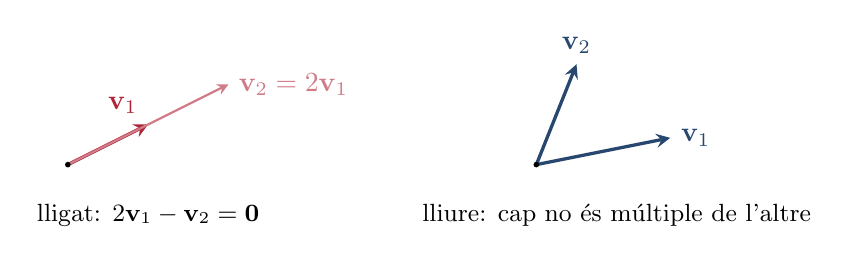
\begin{tikzpicture}[scale=0.85,>=stealth]
\draw[->,very thick,figA] (0,0) -- (1.2,0.6) node[above left]{$\mathbf{v}_{1}$};
\draw[->,thick,figA!60] (0,0) -- (2.4,1.2) node[right]{$\mathbf{v}_{2}=2\mathbf{v}_{1}$};
\fill (0,0) circle (1.2pt);
\node at (1.2,-0.75) {\small lligat: $2\mathbf{v}_{1}-\mathbf{v}_{2}=\mathbf{0}$};
\begin{scope}[xshift=7cm]
\draw[->,very thick,figB] (0,0) -- (2.0,0.4) node[right]{$\mathbf{v}_{1}$};
\draw[->,very thick,figB] (0,0) -- (0.6,1.5) node[above]{$\mathbf{v}_{2}$};
\fill (0,0) circle (1.2pt);
\node at (1.2,-0.75) {\small lliure: cap no és múltiple de l'altre};
\end{scope}
\end{tikzpicture}

{\small\itshape En el pla, dos vectors són linealment dependents exactament quan són proporcionals.}
\end{center}

\begin{teorema}
Assenyalem algunes conseqüències immediates de la definició:

\begin{enumerate}
\item Tot sistema que inclogui el vector $\mathbf{0}$ és lligat.

\item Si s'afegeixen altres vectors a un sistema lligat, el sistema que
resulta és també lligat.

\item Tot sistema que inclogui dos vectors iguals és lligat.

\item El sistema $\left( \mathbf{v}_{1},...,\mathbf{v}_{m}\right) $, amb $%
\mathbf{v}_{1}\neq \mathbf{0}$, és lligat si i només si algun dels seus
vectors és combinació lineal dels que el precedeixen.

\item Perquè un sistema sigui lligat és necessari i suficient que existeixi un
subsistema propi equivalent al sistema considerat.
\end{enumerate}

\end{teorema}
\begin{prova}
(1.) Consisteix a triar tots els coeficients iguals a zero, tret del que
multiplical vector $\mathbf{0}$.

(2.) Consisteix a triar, per exemple, els coeficients nuls per als nous
vectors.

(3.) Suposem el sistema $(\mathbf{v}_{1},...,\mathbf{v}_{m})$ en què
per a certs $i,j$, amb $i\neq j$ i $1\leq i<j\leq m$, es compleix $\mathbf{v}%
_{i}=\mathbf{v}_{j}$. Aleshores, és clar que 
\begin{equation*}
0\mathbf{v}_{1}+\cdots +1\mathbf{v}_{i}+\cdots +(-1)\mathbf{v}_{j}+\cdots +0%
\mathbf{v}_{m}=\mathbf{0}
\end{equation*}%
el que significa que el sistema considerat és lligat.

(4.) Si el sistema $(\mathbf{v}_{1},...,\mathbf{v}_{m})$ de $E$ és
lligat, aleshores existeix una successió finita d'escalars $\left( \lambda
_{1},...,\lambda _{m}\right) $, no tots nuls, tals que%
\begin{equation*}
\lambda _{1}\mathbf{v}_{1}+\cdots +\lambda _{m}\mathbf{v}_{m}=\mathbf{0}
\end{equation*}%
De aquests $\lambda _{i}$ no nuls, escollim el que té el més gran subíndex. Sigui $k=\max \{i:\lambda _{i}\neq 0\}$. Se compleix que $k>1$, ja que de
en cas contrari tindríem $\lambda _{1}\mathbf{v}_{1}=\mathbf{0}$, i com
per hipòtesi $\mathbf{v}_{1}\neq \mathbf{0}$, es deduiria que $%
\lambda _{1}=0$, el que no és possible. Aleshores tenim%
\begin{equation*}
\lambda _{1}\mathbf{v}_{1}+\cdots +\lambda _{k}\mathbf{v}_{k}=\mathbf{0}
\end{equation*}%
i $\lambda _{k}\neq 0$. D'aquesta última relació s’obté%
\begin{equation*}
\mathbf{v}_{k}=-\frac{\lambda _{1}}{\lambda _{k}}\mathbf{v}_{1}-\cdots -%
\frac{\lambda _{k-1}}{\lambda _{k}}\mathbf{v}_{k-1}
\end{equation*}%
és a dir, podem expressar $\mathbf{v}_{k}$ com a combinació lineal de
els vectors que el precedeixen $\mathbf{v}_{1},...,\mathbf{v}_{k-1}$.

Recíprocament, si existeix $\mathbf{v}_{k}$ amb $1\leq k\leq m$ tal que%
\begin{equation*}
\mathbf{v}_{k}=\mu _{1}\mathbf{v}_{1}+\cdots +\mu _{k-1}\mathbf{v}_{k-1}
\end{equation*}%
aleshores%
\begin{equation*}
-\mu _{1}\mathbf{v}_{1}-\cdots -\mu _{k-1}\mathbf{v}_{k-1}+1\mathbf{v}_{k}+0%
\mathbf{v}_{k+1}+\cdots +0\mathbf{v}_{m}=0
\end{equation*}%
el que significa que el sistema $(\mathbf{v}_{1},...,\mathbf{v}_{m})$ és
lligat.

Amb una demostració anàloga es deduiria el teorema que
resulta de substituir la hipòtesi $\mathbf{v}_{1}\neq 0$ per $\mathbf{v}%
_{m}\neq 0$, i la paraula ``preceden'' per ``siguen''.

(5.) Si el sistema $(\mathbf{v}_{1},...,\mathbf{v}_{m})$ de $E$ és
lligat, aleshores existeix una successió finita d'escalars $\left( \lambda
_{1},...,\lambda _{m}\right) $, no tots nuls, tals que%
\begin{equation*}
\lambda _{1}\mathbf{v}_{1}+\cdots +\lambda _{m}\mathbf{v}_{m}=\mathbf{0}
\end{equation*}%
Suposem que $\lambda _{i}\neq 0$, aleshores es té%
\begin{equation*}
\frac{\lambda _{1}}{\lambda _{i}}\mathbf{v}_{1}+\cdots +1\mathbf{v}%
_{i}+\cdots +\frac{\lambda _{m}}{\lambda _{i}}\mathbf{v}_{m}=\mathbf{0}
\end{equation*}%
d’on%
\begin{equation*}
\mathbf{v}_{i}=-\frac{\lambda _{1}}{\lambda _{i}}\mathbf{v}_{1}-\cdots -%
\frac{\lambda _{m}}{\lambda _{i}}\mathbf{v}_{m}
\end{equation*}%
és a dir, $\mathbf{v}_{i}$ és combinació lineal dels vectors $%
\mathbf{v}_{1},...,\mathbf{v}_{i-1},\mathbf{v}_{i+1},...,\mathbf{v}_{m}$.
Aleshores, per aplicacions successives de T1, es té%
\begin{equation*}
\left( \mathbf{v}_{1},...,\mathbf{v}_{i},...,\mathbf{v}_{m}\right) \sim
\left( \mathbf{v}_{1},...,\mathbf{v}_{i-1},\mathbf{v}_{i+1},...,\mathbf{v}%
_{m},\mathbf{v}_{i}\right)
\end{equation*}%
i, pel teorema 10, es té%
\begin{equation*}
\left( \mathbf{v}_{1},...,\mathbf{v}_{i-1},\mathbf{v}_{i+1},...,\mathbf{v}%
_{m},\mathbf{v}_{i}\right) \sim \left( \mathbf{v}_{1},...,\mathbf{v}_{i-1},%
\mathbf{v}_{i+1},...,\mathbf{v}_{m}\right)
\end{equation*}%
Per tant,%
\begin{equation*}
\left( \mathbf{v}_{1},...,\mathbf{v}_{i},...,\mathbf{v}_{m}\right) \sim
\left( \mathbf{v}_{1},...,\mathbf{v}_{i-1},\mathbf{v}_{i+1},...,\mathbf{v}%
_{m}\right)
\end{equation*}%
D'aquesta manera s'ha obtingut un subsistema propi equivalent al sistema
original.

El recíproc és evident, ja que si el sistema donat és equivalent a un
subsistema seu, qualsevol vector d’aquest darrer és combinació
lineal dels vectors del sistema i, en conseqüència, el sistema és lligat.
\end{prova}

\begin{observacio}
Del darrer resultat del teorema anterior es dedueix que si en la relació de
dependència%
\begin{equation*}
\lambda _{1}\mathbf{v}_{1}+\cdots +\lambda _{m}\mathbf{v}_{m}=\mathbf{0}
\end{equation*}%
és $\lambda _{i}\neq 0$, aleshores el sistema que s'obté eliminant el vector $%
\mathbf{v}_{i}$ és equivalent al sistema original. Observeu que només es pot
suprimir \textbf{un} vector per cada relació de dependència: un cop eliminat $%
\mathbf{v}_{i}$, la relació anterior deixa de ser una relació entre els
vectors del nou sistema.
\end{observacio}

\begin{definicio}
Direm que el sistema $(\mathbf{v}_{1},...,\mathbf{v}_{m})$ de vectors de
un espai vectorial $E$ és \textbf{lliure} quan no és lligat.

Quan el sistema de vectors $(\mathbf{v}_{1},...,\mathbf{v}_{m})$ de $%
E$ és lliure, també es diu que els vectors $\mathbf{v}%
_{1},...,\mathbf{v}_{m}$ del sistema són \textbf{linealment independents}.
\end{definicio}

\begin{observacio}
Dit d'una altra manera, perquè un sistema $(\mathbf{v}_{1},\mathbf{v}_{2},...,%
\mathbf{v}_{m})$ sigui lliure és necessari i suficient que la relació%
\begin{equation*}
\lambda _{1}\mathbf{v}_{1}+\cdots +\lambda _{m}\mathbf{v}_{m}=\mathbf{0}
\end{equation*}%
es compleixi només si tots els coeficients $\lambda _{i}$ són nuls; la 
única combinació nul·la dels vectors del sistema correspon a
triar tots els coeficients nuls.
\end{observacio}

\begin{teorema}
Assenyalem algunes conseqüències immediates de la definició:

\begin{enumerate}
\item Un vector $\mathbf{v}$ no nul constitueix per si sol un sistema
lliure.

\item Tots els vectors d’un sistema lliure són diferents de $\mathbf{0}$.

\item Tots els vectors d’un sistema lliure són dos a dos diferents.

\item Tot subsistema d’un sistema lliure és també lliure.

\item En la clausura lineal d’un sistema lliure, tot vector pot
escriure's de manera única com a combinació lineal dels vectors
del sistema.

\item Si el sistema $(\mathbf{v}_{1},...,\mathbf{v}_{m})$ és lliure, mientras
que el sistema $(\mathbf{v}_{1},...,\mathbf{v}_{m},\mathbf{w})$, obtingut afegint-hi un vector, és lligat, aleshores el vector $\mathbf{w}$ és
combinació lineal dels vectors $\mathbf{v}_{1},...,\mathbf{v}_{m}$.
\end{enumerate}

\end{teorema}
\begin{prova}
(1.) En efecte,%
\begin{equation*}
\lambda \mathbf{v}=\mathbf{0}\Longrightarrow \lambda =0
\end{equation*}%
ja que la igualtat $\mathbf{v}=\mathbf{0}$ queda excluida.

(2.) Qualsevol sistema que conté al vector $\mathbf{0}$ és lligat.

(3.) Qualsevol sistema que conté dos vectors iguals és lligat.

(4.) En efecte, si el nou sistema fos lligat, afegint-hi altres
vectors continuaria essent un sistema lligat.

(5.) Suposem que el sistema $\left( \mathbf{v}_{1},...,\mathbf{v}%
_{m}\right) $ és lliure. Sigui $\mathbf{v}\in \left\langle \mathbf{v}_{1},...,%
\mathbf{v}_{m}\right\rangle $ i suposem que $\mathbf{v}$ pudiera
escriure's de dues maneres:%
\begin{equation*}
\mathbf{v}=\lambda _{1}\mathbf{v}_{1}+\cdots +\lambda _{m}\mathbf{v}_{m}=\mu
_{1}\mathbf{v}_{1}+\cdots +\mu _{m}\mathbf{v}_{m}
\end{equation*}%
Aleshores, tindríem%
\begin{equation*}
(\lambda _{1}-\mu _{1})\mathbf{v}_{1}+\cdots +(\lambda _{m}-\mu _{m})\mathbf{%
v}_{m}=\mathbf{0}
\end{equation*}%
i per ser independents els vectors $\mathbf{v}_{i}$ hauríem de%
\begin{equation*}
\lambda _{i}-\mu _{i}=0\,\ (i=1,...,m)
\end{equation*}%
En conseqüència, les dues descomposiciones coinciden.

(6.) Per ser el sistema $(\mathbf{v}_{1},...,\mathbf{v}_{m},\mathbf{w})$
lligat, tindrem la següent relació lineal%
\begin{equation*}
\lambda _{1}\mathbf{v}_{1}+\cdots +\lambda _{m}\mathbf{v}_{m}+\mu \mathbf{w}=%
\mathbf{0}
\end{equation*}%
on $\mu \neq 0$ ja que el sistema $(\mathbf{v}_{1},...,\mathbf{v}_{m})$
és lliure. Per consegüent podem aïllar $\mathbf{w}$, el que demostra
la afirmació.
\end{prova}

\begin{observacio}
Fem les observacions següents:

\begin{enumerate}
\item Del \textbf{teorema 7} i del \textbf{teorema 15 (5)} es dedueix
immediatament el resultat següent: si el sistema $\left( \mathbf{v}%
_{1},...,\mathbf{v}_{m}\right) $ és lliure, aleshores%
\begin{equation*}
\left\langle \mathbf{v}_{1},...,\mathbf{v}_{m}\right\rangle =\left\langle 
\mathbf{v}_{1}\right\rangle \oplus \cdots \oplus \left\langle \mathbf{v}%
_{m}\right\rangle
\end{equation*}

\item Les nocions de dependència i independència lineal es generalitzen per a
qualsevol família $(\mathbf{v}_{i})_{i\in I}$ de vectors de $E$.
Una família $(\mathbf{v}_{i})_{i\in I}$ de vectors de $E$ es dirá lliure si ho és tota subfamília finita. Una família s’anomenará
lligada si no és lliure. Esto significa que almenys hi ha una subfamília finita
que no és lliure.
\end{enumerate}
\end{observacio}

\begin{teorema}
Si l’espai vectorial $E$ és generat pel sistema $(\mathbf{v%
}_{1},...,\mathbf{v}_{m})$, i $E$ conté $k$ vectors linealment
independents, aleshores $k\leq m$.

\end{teorema}
\begin{prova}
Suposem que $\mathbf{w}_{1},...,\mathbf{w}_{k}$ són vectors linealment
independents de $E$. És clar que el sistema $\left( \mathbf{w}%
_{1},\mathbf{v}_{1},...,\mathbf{v}_{m}\right) $ és generador de $E$%
. Com que $E=\left\langle \mathbf{v}_{1},...,\mathbf{v}%
_{m}\right\rangle $, $\mathbf{w}_{1}$ és combinació lineal de $\mathbf{v%
}_{1},...,\mathbf{v}_{m}$. Per tant, $\left( \mathbf{w}_{1},\mathbf{v}%
_{1},...,\mathbf{v}_{m}\right) $ és lligat, i pel \textbf{teorema 14 (4)}
existeix un vector que és combinació lineal dels precedents, que no és 
$\mathbf{w}_{1}$ ja que $\mathbf{w}_{1}\neq 0$ (per pertànyer a un sistema
lliure); sigui aquest vector $\mathbf{v}_{i}$. Suprimiéndolo obtenim altre
sistema generador equivalent, és a dir,%
\begin{equation*}
E=\left\langle \mathbf{v}_{1},...,\mathbf{v}_{i},...,\mathbf{v}%
_{m}\right\rangle =\left\langle \mathbf{w}_{1},\mathbf{v}_{1},...,\mathbf{v}%
_{i-1},\mathbf{v}_{i+1},...,\mathbf{v}_{m}\right\rangle
\end{equation*}%
També serà generador el sistema $\left( \mathbf{w}_{2},\mathbf{w}%
_{1},\mathbf{v}_{1},...,\mathbf{v}_{i-1},\mathbf{v}_{i+1},...,\mathbf{v}%
_{m}\right) $ que al seu torn és lligat. Tornant a aplicar el \textbf{teorema
14 (4)} podem suprimir un altre vector $\mathbf{v}_{j}$, que no és $\mathbf{w}%
_{2}$ ni $\mathbf{w}_{1}$ perquè $(\mathbf{w}_{1},\mathbf{w}_{2})$ és un
sistema lliure. Repetint aquest procés resulta que, si fuese $k>m$, el
sistema $\left( \mathbf{w}_{m},...,\mathbf{w}_{1}\right) $ seria
generador; en conseqüència, $\mathbf{w}_{m+1}$ seria combinació lineal de $%
\mathbf{w}_{1},...,\mathbf{w}_{m}$ i el sistema $\left( \mathbf{w}_{1},...,%
\mathbf{w}_{m+1}\right) $ seria lligat, contra la hipòtesi.
\end{prova}

\begin{exemple}
Demostreu que dos vectors d’un espai vectorial $E$ són
linealment dependents si i només si un d'ells és un múltiple escalar
de l'altre.

\end{exemple}
\begin{solucio}
Siguin $\mathbf{v}_{1},\mathbf{v}_{2}$ dos vectors linealment dependents de $%
E$. Aleshores existeix una relació de dependència d'aquests
vectors%
\begin{equation*}
\lambda _{1}\mathbf{v}_{1}+\lambda _{2}\mathbf{v}_{2}=\mathbf{0}
\end{equation*}%
amb algún $\lambda _{i}\neq 0$. Suposem que $\lambda _{1}\neq 0$,
aleshores%
\begin{equation*}
1\mathbf{v}_{1}+\frac{\lambda _{2}}{\lambda _{1}}\mathbf{v}_{2}=\mathbf{0}
\end{equation*}%
d’on%
\begin{equation*}
\mathbf{v}_{1}=-\frac{\lambda _{2}}{\lambda _{1}}\mathbf{v}_{2}
\end{equation*}%
amb el que $\mathbf{v}_{1}$ és múltiple escalar de $\mathbf{v}_{2}$.
Recíprocament, si $\mathbf{v}_{1}=\lambda \mathbf{v}_{2}$ per a algun $%
\lambda \in \mathbb{K}$, aleshores%
\begin{equation*}
1\mathbf{v}_{1}+(-\lambda )\mathbf{v}_{2}=\mathbf{0}
\end{equation*}%
és una relació de dependència amb el coeficient de $\mathbf{v}_{1}$ diferent
de zero i, per tant, $\mathbf{v}_{1}$ i $\mathbf{v}_{2}$ són linealment
dependents.
\end{solucio}

\begin{exemple}
Determineu si el sistema $(\mathbf{v}_{1},\mathbf{v}_{2},\mathbf{v}_{3})$ de 
$\mathbb{R}^{3}$ és o no lliure, essent $\mathbf{v}_{1}=(1,2,3),\mathbf{v}%
_{2}=(0,1,2),\mathbf{v}_{3}=(-2,0,1)$.

\end{exemple}
\begin{solucio}
Suposem que%
\begin{equation*}
\lambda _{1}\mathbf{v}_{1}+\lambda _{2}\mathbf{v}_{2}+\lambda _{3}\mathbf{v}%
_{3}=\mathbf{0}
\end{equation*}%
Introduint els seus components, es té%
\begin{equation*}
\lambda _{1}(1,2,3)+\lambda _{2}(0,1,2)+\lambda _{3}(-2,0,1)=(0,0,0)
\end{equation*}%
o bien%
\begin{equation*}
(\lambda _{1}-2\lambda _{3},2\lambda _{1}+\lambda _{2},3\lambda
_{1}+2\lambda _{2}+\lambda _{3})=(0,0,0)
\end{equation*}%
Igualant components, s’obté el següent sistema:%
\begin{equation*}
\left. 
\begin{array}{r}
\lambda _{1}-2\lambda _{3}=0 \\ 
2\lambda _{1}+\lambda _{2}=0 \\ 
3\lambda _{1}+2\lambda _{2}+\lambda _{3}=0%
\end{array}%
\right\}
\end{equation*}%
resolent-lo, s’obté, $\lambda _{1}=0,\lambda _{2}=0,\lambda _{3}=0$%
. Per tant, el sistema és lliure.
\end{solucio}

\begin{exemple}
Demostreu que el sistema $(1+x-2x^{2},2+5x-x^{2},x+x^{2})$ de $\mathbb{R}_{2}%
\left[ x\right] $ és lligat. Escriviu una relació de dependència.

\end{exemple}
\begin{solucio}
Suposem que%
\begin{equation*}
\lambda _{1}(1+x-2x^{2})+\lambda _{2}(2+5x-x^{2})+\lambda _{3}(x+x^{2})=%
\mathbf{0}
\end{equation*}%
aleshores%
\begin{equation*}
(\lambda _{1}+2\lambda _{2})+(\lambda _{1}+5\lambda _{2}+\lambda
_{3})x+(-2\lambda _{1}-\lambda _{2}+\lambda _{3})x^{2}=\mathbf{0}
\end{equation*}%
Pel principi d'identitat de polinomis, s’obté el sistema següent:%
\begin{equation*}
\begin{array}{r}
\lambda _{1}+2\lambda _{2}=0 \\ 
\lambda _{1}+5\lambda _{2}+\lambda _{3}=0 \\ 
-2\lambda _{1}-\lambda _{2}+\lambda _{3}=0%
\end{array}%
\end{equation*}%
És fàcil comprovar que aquest sistema és compatible indeterminat i, en
conseqüència, el sistema és lligat. Les seves solucions són, $\lambda
_{1}=-2\lambda _{2},\lambda _{2}=\lambda _{2},\lambda _{3}=-3\lambda _{2}$.
Prenent $\lambda _{2}=-1$, s’obté $\lambda _{1}=2$ i $\lambda _{3}=3$.
Per tant,%
\begin{equation*}
2(1+x-2x^{2})+(-1)(2+5x-x^{2})+3(x+x^{2})=\mathbf{0}
\end{equation*}%
és una relació de dependència.
\end{solucio}

\section{Bases d’un espai vectorial de dimensió finita}

\begin{definicio}
S’anomena \textbf{base} d’un espai vectorial \thinspace $E$ a
tota família lliure (finita o no) que engendra $E$.
\end{definicio}

\begin{definicio}
Es diu que un espai vectorial $E$ és de \textbf{dimensió
finita} si admet almenys una família finita que engendra $E$.
\end{definicio}

\begin{observacio}
Dit d'una altra manera, $E$ és de dimensió finita si existeix un
família finita $\left( \mathbf{v}_{1},...,\mathbf{v}_{m}\right) $ de $%
E$ tal que%
\begin{equation*}
E=\left\langle \mathbf{v}_{1},...,\mathbf{v}_{m}\right\rangle
\end{equation*}
\end{observacio}

\begin{teorema}
Tot espai vectorial $E\neq \left\{ \mathbf{0}\right\} $ de
dimensió finita posee una base.

\end{teorema}
\begin{prova}
Suposem que $E=\left\langle \mathbf{v}_{1},...,\mathbf{v}%
_{m}\right\rangle $. Si el sistema $\left( \mathbf{v}_{1},...,\mathbf{v}%
_{m}\right) $ és lliure, formen una base i el teorema queda demostrat. En
cas contrari, existeix almenys un vector $\mathbf{v}_{i}$ que és combinació lineal dels altres. Aleshores%
\begin{equation*}
E=\left\langle \mathbf{v}_{1},...,\mathbf{v}_{m}\right\rangle
=\left\langle \mathbf{v}_{1},...,\mathbf{v}_{i-1},\mathbf{v}_{i+1},...,%
\mathbf{v}_{m}\right\rangle
\end{equation*}%
Apliquem de nou el mateix raonament al nou sistema 
\begin{equation*}
\left( \mathbf{v}_{1},...,\mathbf{v}_{i-1},\mathbf{v}_{i+1},...,\mathbf{v}%
_{m}\right)
\end{equation*}%
Si és lliure, constitueix una base i, si no ho és, suprimim un altre vector,
i es dedueix un tercer sistema generador. Repetint un nombre finit de
vegades aquest procés, arribarem a un sistema lliure i generador de $E$%
, és a dir, a una base, o suprimirem tots els vectors. Ara bé, en
aquest segon cas seria $E=\left\langle \mathbf{0}%
\right\rangle =\left\{ \mathbf{0}\right\} $, el que no seria possible
per hipòtesi.
\end{prova}

\begin{observacio}
Fem les observacions següents:

\begin{enumerate}
\item De la demostració del teorema anterior es dedueix de manera
immediata el resultat següent: tot sistema generador de $E$
conté un subsistema lliure equivalent.

\item En general, es demostra que tot espai vectorial (de dimensió
finita o no) admet una base.
\end{enumerate}
\end{observacio}

\begin{teorema}
Totes les bases d’un espai vectorial $E$ de dimensió finita
són finites i tenen el mateix nombre de vectors.

\end{teorema}
\begin{prova}
Siguin $\mathcal{B}_{1}$ i $\mathcal{B}_{2}$ dues bases qualssevol de $%
E$, deducidas o no d’un sistema generador $(\mathbf{v}_{1},...,%
\mathbf{v}_{m})$ de $E$. El \textbf{teorema 16} prova que cadascuna
d'elles té un nombre finit de vectors; $n_{1}$ per a $\mathcal{B}%
_{1}$ i $n_{2}$ per a $\mathcal{B}_{2}$, amb $n_{1}\leq m$ i $n_{2}\leq m$.
D’altra banda, cada base constitueix una família lliure i generatriz de $%
E$. Considerem $\mathcal{B}_{1}$ com família generatriz i $%
\mathcal{B}_{2}$ com família lliure, pel \textbf{teorema 16}, és $%
n_{2}\leq n_{1}$. Repetint de nou el mateix raonament, canviant el
paper de les dues bases, s’arriba a que $n_{1}\leq n_{2}$. Per consegüent, $%
n_{1}=n_{2}$.
\end{prova}

\begin{observacio}
En general, es demostra que totes les bases d’un espai vectorial (de
dimensió finita o no) són equipotentes (de la mateixa cardinalidad).
\end{observacio}

\begin{definicio}
El nombre de vectors de qualsevol base finita d’un espai vectorial $%
E$ s’anomena \textbf{dimensió} de $E$ i es denota per $%
\dim E$. Direm que $E$ és de \textbf{dimensió
infinita} si no té bases finites.
\end{definicio}

\begin{observacio}
El subespai nul $\left\{ \mathbf{0}\right\} $ no posee base alguna, ja
que la família $\left( \mathbf{0}\right) $ és lligada, però es admet que: 
\begin{equation*}
\dim \left\{ \mathbf{0}\right\} =0
\end{equation*}
\end{observacio}

\begin{corollari}
En un espai vectorial de dimensió finita, la dimensió coincide
amb el nombre màxim de vectors linealment independents de
qualsevol sistema lliure, i també amb el nombre mínim de
vectors de qualsevol sistema generador.

\end{corollari}
\begin{prova}
És una conseqüència immediata del \textbf{teorema 16}.
\end{prova}

\begin{corollari}
En un espai vectorial de dimensió finita, tota família lliure de $%
E$ pot completar-se fins a obtenir una base.

\end{corollari}
\begin{prova}
Sigui $(\mathbf{v}_{1},...,\mathbf{v}_{n})$ una base i $\left( \mathbf{w}%
_{1},...,\mathbf{w}_{k}\right) $ una família lliure de $E$, aleshores
per l’\textbf{teorema 16} es poden substituir $k$ vectors $\mathbf{v}_{i}$
pels $\mathbf{w}_{j}$ de manera que la família $(\mathbf{w}_{1},...,\mathbf{%
w}_{k},\mathbf{v}_{i_{1}},...,\mathbf{v}_{i_{n-k}})$ sigui una base de $%
\mathbf{E}$.
\end{prova}

\begin{corollari}
Perquè un sistema de $n$ vectors sigui una base d’un espai vectorial de
dimensió $n$, és suficient que el sistema sigui generador de $E$
o que sigui lliure.

\end{corollari}
\begin{prova}
Pel \textbf{corol·lari 3}, qualsevol sistema lliure de $n$ vectors es
pot completar fins a obtenir una base. Ara bé, totes les bases de l'
espai tenen $n$ vectors pel \textbf{teorema 18}. Per tant, el
sistema és una base. D'altra banda, qualsevol sistema generador de $n$
vectors d’un espai vectorial de dimensió $n$ no és lligada, ja que, en
cas contrari, pel \textbf{teorema 14 (5)}, existiria un subsistema
propi generador, la qual cosa és impossible pel fet que el nombre mínim de vectors de qualsevol sistema generador és $n$, segons el 
\textbf{corol·lari 2}.
\end{prova}

\begin{definicio}
S’anomenan \textbf{coordenades d’un vector} $\mathbf{v}$ d’un espai
vectorial $E$ \textbf{respecte de la base} $(\mathbf{v}_{1},...,%
\mathbf{v}_{n})$ a la única família finita d'escalars $(\lambda
_{1},...,\lambda _{n})$ tals que%
\begin{equation*}
\mathbf{v}=\lambda _{1}\mathbf{v}_{1}+\cdots +\lambda _{n}\mathbf{v}_{n}
\end{equation*}
\end{definicio}

\begin{observacio}
Aquesta última definició té sentit en virtut del \textbf{teorema
15 (5)}.
\end{observacio}

\begin{exemple}
L'espai geomètric ordinari és de tres dimensions, perquè, elegits
tres vectors no coplanaris (no situats en l’mateix pla) $%
\overrightarrow{OA},\overrightarrow{OB},\overrightarrow{OC}$, sabem que
tot vector $\overrightarrow{OM}$ pot escriure’s com segueix:%
\begin{equation*}
\overrightarrow{OM}=\lambda \overrightarrow{OA}+\mu \overrightarrow{OB}+\nu 
\overrightarrow{OC}
\end{equation*}
\end{exemple}

\begin{exemple}
L'espai $\mathbb{K}^{n}$ dels vectors que són $n$-tuples d’elements $%
\mathbb{K}$ és de dimensió $n$. En efecte, considerem els $n$
vectors següents:%
\begin{equation*}
\begin{array}{c}
\mathbf{e}_{1}=(1,0,...,0) \\ 
\mathbf{e}_{2}=(0,1,...,0) \\ 
\vdots \\ 
\mathbf{e}_{n}=(0,0,...,1)%
\end{array}%
\end{equation*}%
dels quals el $i$-ésimo, $\mathbf{e}_{i}$, té component $i$-ésima igual a $1$ i el resto, igual a $0$. El $(\mathbf{e}_{1},%
\mathbf{e}_{2},...,\mathbf{e}_{n})$ és generador de $\mathbb{K}^{n}$, ja que
qualsevol vector $\mathbf{v}=(\lambda _{1},\lambda _{2},...,\lambda _{n})$
de $\mathbb{K}^{n}$ pot escriure’s com segueix:%
\begin{equation*}
\mathbf{v}=\lambda _{1}\mathbf{e}_{1}+\lambda _{2}\mathbf{e}_{2}+\cdots
+\lambda _{n}\mathbf{e}_{n}
\end{equation*}

A més, aquest sistema és lliure. En efecte, la relació%
\begin{equation*}
\lambda _{1}\mathbf{e}_{1}+\lambda _{2}\mathbf{e}_{2}+\cdots +\lambda _{n}%
\mathbf{e}_{n}=\mathbf{0}
\end{equation*}%
només és possible si $\lambda _{i}=0$ per a tot $1\leq i\leq n$.

La base introducida d’aquesta forma, associada de manera particularmente
sencilla a la definició de $\mathbb{K}^{n}$ s’anomena \textbf{base
natural}.
\end{exemple}

\begin{exemple}
Proveu que els vectors de la família $\mathcal{S}$, essent 
\begin{equation*}
\mathcal{S}=((2,1,1),(1,3,1),(-2,1,3))
\end{equation*}
formen una base de $\mathbb{R}^{3}$.

\end{exemple}
\begin{solucio}
Sabem que la dimensió de $\mathbb{R}^{3}$ és tres. Pel \textbf{%
corol·lari 2}, és suficient proveu que $\mathcal{S}$ és lliure. En efecte,
suposem que%
\begin{equation*}
\lambda (2,1,1)+\mu (1,3,1)+\nu (-2,1,3)=(0,0,0)
\end{equation*}%
és a dir,%
\begin{equation*}
(2\lambda +\mu -2\nu ,\lambda +3\mu +\nu ,\lambda +\mu +3\nu )=(0,0,0)
\end{equation*}%
Per igualació dels seus components s’obté el següent sistema:%
\begin{equation*}
\left. 
\begin{array}{r}
2\lambda +\mu -2\nu =0 \\ 
\lambda +3\mu +\nu =0 \\ 
\lambda +\mu +3\nu =0%
\end{array}%
\right\}
\end{equation*}%
la solució del qual és $\nu =0,\lambda =0,\mu =0$. Per tant, $\mathcal{S}$ és
una base de $\mathbb{R}^{3}$.
\end{solucio}

\begin{exemple}
Completar la següent família lliure $(\mathbf{v}_{1},\mathbf{v}_{2},\mathbf{%
v}_{3})$ per a formar una base de $\mathbb{R}^{4}$, essent $\mathbf{v}%
_{1}=(1,1,-1,1),\mathbf{v}_{2}=(1,1,0,1),\mathbf{v}_{3}=(1,2,1,1)$.

\end{exemple}
\begin{solucio}
Sabem que la família $(\mathbf{e}_{1},\mathbf{e}_{2},\mathbf{e}_{3},%
\mathbf{e}_{4})$ és una base de $\mathbb{R}^{4}$, essent $\mathbf{e}%
_{1}=(1,0,0,0),\mathbf{e}_{2}=(0,1,0,0),\mathbf{e}_{3}=(0,0,1,0),\mathbf{e}%
_{4}=(0,0,0,1)$. Tenim%
\begin{equation*}
\mathbf{v}_{1}=1\mathbf{e}_{1}+1\mathbf{e}_{2}+(-1)\mathbf{e}_{3}+1\mathbf{e}%
_{4}
\end{equation*}%
d’on%
\begin{equation*}
\mathbf{e}_{1}=\mathbf{v}_{1}-\mathbf{e}_{2}+\mathbf{e}_{3}-\mathbf{e}_{4}
\end{equation*}%
Per tant,%
\begin{equation*}
(\mathbf{e}_{1},\mathbf{e}_{2},\mathbf{e}_{3},\mathbf{e}_{4})\sim (\mathbf{v}%
_{1},\mathbf{e}_{2},\mathbf{e}_{3},\mathbf{e}_{4})
\end{equation*}%
Tenim%
\begin{equation*}
\mathbf{v}_{2}=1\mathbf{v}_{1}+0\mathbf{e}_{2}+1\mathbf{e}_{3}+0\mathbf{e}%
_{4}
\end{equation*}%
d’on%
\begin{equation*}
\mathbf{e}_{3}=-\mathbf{v}_{1}+\mathbf{v}_{2}
\end{equation*}%
Per tant,%
\begin{equation*}
(\mathbf{v}_{1},\mathbf{e}_{2},\mathbf{e}_{3},\mathbf{e}_{4})\sim (\mathbf{v}%
_{1},\mathbf{e}_{2},\mathbf{v}_{2},\mathbf{e}_{4})
\end{equation*}%
Finalment, es té%
\begin{equation*}
\mathbf{v}_{3}=(-1)\mathbf{v}_{1}+1\mathbf{e}_{2}+2\mathbf{v}_{2}+0\mathbf{e}%
_{4}
\end{equation*}%
d’on%
\begin{equation*}
\mathbf{e}_{2}=\mathbf{v}_{1}-2\mathbf{v}_{2}+\mathbf{v}_{3}
\end{equation*}%
Per tant,%
\begin{equation*}
(\mathbf{v}_{1},\mathbf{e}_{2},\mathbf{v}_{2},\mathbf{e}_{4})\sim (\mathbf{v}%
_{1},\mathbf{v}_{3},\mathbf{v}_{2},\mathbf{e}_{4})
\end{equation*}%
A més, es compleix%
\begin{equation*}
(\mathbf{v}_{1},\mathbf{v}_{3},\mathbf{v}_{2},\mathbf{e}_{4})\sim (\mathbf{v}%
_{1},\mathbf{v}_{2},\mathbf{v}_{3},\mathbf{e}_{4})
\end{equation*}%
Per consegüent, 
\begin{equation*}
(\mathbf{e}_{1},\mathbf{e}_{2},\mathbf{e}_{3},\mathbf{e}_{4})\sim (\mathbf{v}%
_{1},\mathbf{v}_{2},\mathbf{v}_{3},\mathbf{e}_{4})
\end{equation*}%
i, en conseqüència, $(\mathbf{v}_{1},\mathbf{v}_{2},\mathbf{v}_{3},\mathbf{e}%
_{4})$ és una base de $\mathbb{R}^{4}$.
\end{solucio}

\begin{exemple}
El conjunt dels polinomis en una indeterminada $x$ amb coeficients en
un cos commutatiu $\mathbb{K}$ és un espai vectorial sobre $\mathbb{K}$
que denotem per $\mathbb{K}\left[ x\right] $. La família $(1,x,x^{2},...)$
és una base de $\mathbb{K}\left[ x\right] $ ja que tot polinomi pot
escriure's com a combinació lineal d’una subfamília finita. Aquest
espai és de dimensió infinita.
\end{exemple}

\begin{exemple}
En l’espai vectorial $\mathbb{C}$ sobre $\mathbb{R}$ la família $(1,i)$
és una base. La família $(1+i,1-i)$ és una altra base.
\end{exemple}

\section{Dimensió d’un subespai vectorial}

\begin{teorema}
Si $E$ és un espai vectorial de dimensió $n$, tot
subespai vectorial $S$ de $E$ és de dimensió finita
i es compleix%
\begin{equation*}
\dim S\leq \dim E
\end{equation*}%
A més%
\begin{equation*}
\dim S=\dim E\text{ \ \ \ implica \ \ }S=E
\end{equation*}

\end{teorema}
\begin{prova}
El nombre de vectors de qualsevol sistema lliure i generador de $E$ està fitat per $n$. Tot sistema lliure i generador de $S$
tindrà com màxim un nombre determinat $m$ de vectors de $%
E$. Per tant, $m\leq n$. Si $m=n$, els vectors d’una base de $%
S$ constituyen un sistema lliure de $n$ vectors de $E$, i
en conseqüència, una base de $E$. Per tant, $S=E$%
. Finalment, si $E=\left\{ \mathbf{0}\right\} $, es té
igualment $S=\left\{ \mathbf{0}\right\} $.
\end{prova}

\begin{teorema}
En un espai vectorial $E$ de dimensió finita, si partimos
una base en dos parts complementàries, les clausures lineals de cadascun
dels sistemes així definits són subespais suplementaris.

\end{teorema}
\begin{prova}
Sigui $\mathcal{B}=(\mathbf{v}_{1},...,\mathbf{v}_{n})$ una base de $E
$. Considerem els sistemes $\mathcal{S}=(\mathbf{v}_{1},...,\mathbf{v}%
_{k}) $ i $S^{\prime }=(\mathbf{v}_{k+1},...,\mathbf{v}_{n})$, i
siguin 
\begin{align*}
S &=\left\langle \mathbf{v}_{1},...,\mathbf{v}_{k}\right\rangle \\
T &=\left\langle \mathbf{v}_{k+1},...,\mathbf{v}_{n}\right\rangle
\end{align*}%
Per construcció, és clar que $S+T=E$. Sigui $%
\mathbf{v}\in S\cap T$, aleshores%
\begin{align*}
\mathbf{v} &=\lambda _{1}\mathbf{v}_{1}+\cdots +\lambda _{k}\mathbf{v}_{k}
\\
\mathbf{v} &=\lambda _{k+1}\mathbf{v}_{k+1}+\cdots +\lambda _{n}\mathbf{v}%
_{n}
\end{align*}%
d’aquí s’obté%
\begin{equation*}
\lambda _{1}\mathbf{v}_{1}+\cdots +\lambda _{k}\mathbf{v}_{k}-\lambda _{k+1}%
\mathbf{v}_{k+1}-\cdots -\lambda _{n}\mathbf{v}_{n}=\mathbf{0}
\end{equation*}%
d’on $\lambda _{i}=0$ per a tot $1\leq i\leq n$, ja que $(\mathbf{v}%
_{1},...,\mathbf{v}_{n})$ és un sistema lliure. Per consegüent, $\mathbf{v}=%
\mathbf{0}$ i, en conseqüència, $S\cap T=\left\{ \mathbf{0}%
\right\} $.
\end{prova}

\begin{teorema}
\label{teorema21}En un espai vectorial $E$ de dimensió $n$,
tot subespai $S$ admet almenys un subespai suplementari $%
T$ i es compleix%
\begin{equation*}
E=S\oplus T\text{ \ \ implica \ \ }\dim E%
=\dim S+\dim T
\end{equation*}

\end{teorema}
\begin{prova}
Sigui $(\mathbf{u}_{1},...,\mathbf{u}_{p})$ una base de $S$. Existe
en $E$ almenys un vector $\mathbf{v}_{1}$ tal que el sistema $(%
\mathbf{u}_{1},...,\mathbf{u}_{p},\mathbf{v}_{1})$ és lliure, ja que, en cas
contrari, els vectors $\mathbf{u}_{i}$ formarien una base de $E$ i tindríem $S=E$ i, en conseqüència, $T%
=\left\{ \mathbf{0}\right\} $. Es repeteix el raonament amb el sistema
lliure $(\mathbf{u}_{1},...,\mathbf{u}_{p},\mathbf{v}_{1})$ que té $p+1$
vectors. Podem afegir-hi un altre vector $\mathbf{v}_{2}$ de manera que s'obtingui un altre sistema lliure $(\mathbf{u}_{1},...,\mathbf{u}_{p},\mathbf{v}%
_{1},\mathbf{v}_{2})$ si $p+1<n$. Aquest procés acaba quan s'hagin
introduït $n-p$ nous vectors, perquè s'haurà obtingut una base de $%
E$. Els vectors del sistema lliure $\left( \mathbf{v}_{1},\mathbf{v}%
_{2},...,\mathbf{v}_{n-p}\right) $ engendran un subespai vectorial $%
T$, la dimensió del qual és $n-p$, i és un suplementari de $S$. Finalment, si $S=\left\{ \mathbf{0}\right\} $, aleshores $%
T=E$.
\end{prova}

\begin{observacio}
Una demostració alternativa basada en resultats anteriors és la
següent: Si $\mathcal{S}$ és una base de $S$, segons el 
\textbf{corol·lari 3} de la secció anterior, existeix un sistema $\mathcal{%
S}^{\prime }$ lliure tal que $(\mathcal{S},\mathcal{S}^{\prime })$ és una
base de $E$. D’aquí, pel \textbf{teorema 20}, els
subespais $S=\left\langle \mathcal{S}\right\rangle $ i $T%
=\left\langle \mathcal{S}^{\prime }\right\rangle $ són suplementaris.
\end{observacio}

\begin{teorema}
Siguin $S$ i $T$ dos subespais vectorials d’un espai
vectorial $E$ de dimensió finita. Aleshores es compleix%
\begin{equation*}
\dim S+\dim T=\dim (S\cap T)+\dim (%
S+T)
\end{equation*}

\end{teorema}
\begin{prova}
Sigui $(\mathbf{u}_{1},...,\mathbf{u}_{p})$ una base de $S\cap 
T$. Pel \textbf{corol·lari 3} de la secció anterior, podem
completar aquesta base fins a obtenir una base de $S$ i una base de $%
T$. Así tenim que $(\mathbf{u}_{1},...,\mathbf{u}_{p},%
\mathbf{u}_{p+1},...,\mathbf{u}_{k})$ és una base de $S$ i $(%
\mathbf{u}_{1},...,\mathbf{u}_{p},\mathbf{v}_{p+1},...,\mathbf{v}_{m})$ és
una base de $T$. Aleshores 
\begin{equation*}
(\mathbf{u}_{1},...,\mathbf{u}_{p},\mathbf{u}_{p+1},...,\mathbf{u}_{k},%
\mathbf{v}_{p+1},...,\mathbf{v}_{m})
\end{equation*}%
constitueix un sistema de generador de $S+T$. Si
demostrem que tots aquests vectors són linealment independents,
haurem obtingut una base de $S+T$ amb un nombre de
vectors que prova la igualtat del enunciado. Suposem%
\begin{equation*}
\sum_{i=1}^{k}\lambda _{i}\mathbf{u}_{i}+\sum_{i=p+1}^{m}\mu _{i}\mathbf{v}%
_{i}=\mathbf{0}
\end{equation*}%
aleshores%
\begin{equation*}
\sum_{i=1}^{k}\lambda _{i}\mathbf{u}_{i}=-\sum_{i=p+1}^{m}\mu _{i}\mathbf{v}%
_{i}
\end{equation*}%
és un vector de $S\cap T$, d’on%
\begin{equation*}
-\sum_{i=p+1}^{m}\mu _{i}\mathbf{v}_{i}=\sum_{j=1}^{p}\nu _{j}\mathbf{u}_{j}
\end{equation*}%
és a dir%
\begin{equation*}
\sum_{j=1}^{p}\nu _{j}\mathbf{u}_{j}+\sum_{i=p+1}^{m}\mu _{i}\mathbf{v}_{i}=%
\mathbf{0}
\end{equation*}%
i, com que $(\mathbf{u}_{1},...,\mathbf{u}_{p},\mathbf{v}_{p+1},...,\mathbf{%
v}_{m})$ és una base de $T$, es dedueix $\nu _{j}=0$ $(j=1,...,p)$ i 
$\mu _{i}=0\,\ (i=p+1,...,m)$. Per tant,%
\begin{equation*}
\sum_{i=1}^{k}\lambda _{i}\mathbf{u}_{i}=\mathbf{0}
\end{equation*}%
i, com que $(\mathbf{u}_{1},...,\mathbf{u}_{p},\mathbf{u}_{p+1},...,\mathbf{%
u}_{k})$ és una base de $S$, es dedueix $\lambda _{i}=0$ $%
(i=1,...,k) $.
\end{prova}

\begin{corollari}
En les mateixes condicions del teorema anterior, es compleix%
\begin{equation*}
\dim (S\oplus T)=\dim S+\dim T
\end{equation*}%
En aquest cas, la reunió d’una base de $S$ i d’una base de $%
T$ da una base de $S\oplus T$.

\end{corollari}
\begin{prova}
És immediat, sabent que quan la suma és directa, $S\cap 
T=\left\{ \mathbf{0}\right\} $; a més, $\dim \left\{ \mathbf{0}%
\right\} =0$
\end{prova}

\begin{corollari}
La suma $S+T$ de dos subespais és directa si i només
si $\dim S+\dim T=\dim (S+T)$.

\end{corollari}
\begin{prova}
És immediat a partir del teorema precedent.
\end{prova}

\begin{exemple}
Determineu una base per a la suma i la intersecció dels subespais $%
S$ i $T$ de $\mathbb{R}^{4}$ generats pels conjunts 
$\{(1,2,1,0),(-1,1,1,1)\}$ i $\{(2,-1,0,1),(1,-1,3,7)\}$ respectivament.

\end{exemple}
\begin{solucio}
És clar que $dim\,S=2$ i $dim\,T=2$. Un vector $%
(x,y,z,t)\in S\cap T$ ha de complir%
\begin{equation*}
(x,y,z,t)=\alpha (1,2,1,0)+\beta (-1,1,1,1)=\lambda (2,-1,0,1)+\mu (1,-1,3,7)
\end{equation*}%
és a dir%
\begin{equation*}
(\alpha -\beta ,2\alpha +\beta ,\alpha +\beta ,\beta )=(2\lambda +\mu
,-\lambda -\mu ,3\mu ,\lambda +7\mu )
\end{equation*}%
Per tant, s’obté el següent sistema%
\begin{equation*}
\left. 
\begin{array}{rrrr}
E_{1}: & \alpha -\beta & = & 2\lambda +\mu \\ 
E_{2}: & 2\alpha +\beta & = & -\lambda -\mu \\ 
E_{3}: & \alpha +\beta & = & 3\mu \\ 
E_{4}: & \beta & = & \lambda +7\mu%
\end{array}%
\right\}
\end{equation*}%
Efectuant les transformacions indicades%
\begin{equation*}
\begin{array}{cc}
E_{1}+E_{2}: & 3\alpha =\lambda \\ 
E_{3}: & \beta =\lambda +7\mu%
\end{array}%
\end{equation*}%
Substituint aquests resultats en $E_{3}$ es té%
\begin{equation*}
\lambda =-3\mu
\end{equation*}%
Per tant, $\alpha =-\mu ,\beta =4\mu $ i $\lambda =-3\mu $. D’aquí, es
té%
\begin{equation*}
(x,y,z,t)=-\mu (1,2,1,0)+4\mu (-1,1,1,1)=\mu (-5,2,3,4)
\end{equation*}%
Per tant,%
\begin{equation*}
S\cap T=\left\langle (-5,2,3,4)\right\rangle
\end{equation*}%
i, en conseqüència, $((-5,2,3,4))$ és una base de $S\cap T$
i $dim\,(S\cap T)=1$. Per la fórmula del \textbf{%
teorema 22}, es dedueix%
\begin{equation*}
dim\,(S+T)=dim\,S+dim\,T-dim\,(S%
\cap T)=2+2-1=3
\end{equation*}%
Sabem que%
\begin{equation*}
S+T=\left\langle
(1,2,1,0),(-1,1,1,1),(2,-1,0,1),(1,-1,3,7)\right\rangle
\end{equation*}%
i pel resultat anterior ha de ser un dels vectors generadors
dependent dels altres. Per trobar-lo apliquem successives
transformacions elementals amb objecte de trobar un sistema equivalent
lliure.%
\begin{equation*}
\begin{array}{cccc}
\mathbf{v}_{1} & \mathbf{v}_{2} & \mathbf{v}_{3} & \mathbf{v}_{4} \\ 
1 & -1 & 2 & 1 \\ 
2 & 1 & -1 & -1 \\ 
1 & 1 & 0 & 3 \\ 
0 & 1 & 1 & 7%
\end{array}%
\sim 
\begin{array}{cccc}
\mathbf{v}_{1} & \mathbf{v}_{2}+\mathbf{v}_{1}=\mathbf{u}_{2} & \mathbf{v}%
_{3}-2\mathbf{v}_{1}=\mathbf{u}_{3} & \mathbf{v}_{4}-\mathbf{v}_{1}=\mathbf{u%
}_{4} \\ 
1 & 0 & 0 & 0 \\ 
2 & 3 & -5 & -3 \\ 
1 & 2 & -2 & 2 \\ 
0 & 1 & 1 & 7%
\end{array}%
\sim
\end{equation*}%
\begin{equation*}
\begin{array}{cccc}
\mathbf{v}_{1} & \mathbf{u}_{2} & 5\mathbf{u}_{2}+3\mathbf{u}_{3}=\mathbf{w}%
_{3} & \mathbf{u}_{4}+\mathbf{u}_{2}=\mathbf{w}_{4} \\ 
1 & 0 & 0 & 0 \\ 
2 & 3 & 0 & 0 \\ 
1 & 2 & 4 & 4 \\ 
0 & 1 & 8 & 8%
\end{array}%
\sim 
\begin{array}{cccc}
\mathbf{v}_{1} & \mathbf{u}_{2} & \mathbf{w}_{3} & \mathbf{w}_{4}-\mathbf{w}%
_{3} \\ 
1 & 0 & 0 & 0 \\ 
2 & 3 & 0 & 0 \\ 
1 & 2 & 4 & 0 \\ 
0 & 1 & 8 & 0%
\end{array}%
\end{equation*}%
Per consegüent%
\begin{equation*}
S+T=\left\langle (1,2,1,0),(0,3,2,1),(0,0,4,8)\right\rangle
\end{equation*}%
i una base de $S+T$ és $((1,2,1,0),(0,3,2,1),(0,0,4,8))$.
\end{solucio}

\section{Espai vectorial quocient}

Sigui $E$ un espai vectorial i $F$ un subespai vectorial
de $E$.

\begin{definicio}
Diem que $\mathbf{u},\mathbf{v}\in E$ estan \textbf{%
relacionats mòdul} $F$ si $\mathbf{u}-\mathbf{v}\in F
$. Simbòlicament, escrivim%
\begin{equation*}
\mathbf{u}\equiv \mathbf{v}\operatorname{mod}F\text{ si i només si }%
\mathbf{u}-\mathbf{v}\in F
\end{equation*}
\end{definicio}

\begin{teorema}
Aquesta relació és una congruència sobre $E$.

\end{teorema}
\begin{prova}
Primer provarem que $\equiv $ és una relació d'equivalència. En
efecte, per a tot $\mathbf{u},\mathbf{v},\mathbf{w}\in E$ es té:
(1) $\mathbf{u}\equiv \mathbf{u}$ $\operatorname{mod}F$, ja que $\mathbf{u}-%
\mathbf{u}=\mathbf{0}\in F$ ($\equiv $ és reflexiva); (2) si $%
\mathbf{u}\equiv \mathbf{v}$ $\operatorname{mod}F$, és a dir, $\mathbf{u}-%
\mathbf{v}\in F$, aleshores $-(\mathbf{u}-\mathbf{v})=\mathbf{v}-%
\mathbf{u}\in F$, és a dir, $\mathbf{v}\equiv \mathbf{u}$ $\operatorname{mod}F$ ($\equiv $ és simètrica); (3) si $\mathbf{u}\equiv \mathbf{v%
}$ $\operatorname{mod}F$ i $\mathbf{v}\equiv \mathbf{w}$ $\operatorname{mod}F$, és a dir, si $\mathbf{u}-\mathbf{v}\in F$ i $\mathbf{v}-%
\mathbf{w}\in F$, aleshores $\left( \mathbf{u}-\mathbf{v}\right)
+\left( \mathbf{v}-\mathbf{w}\right) =\mathbf{u}-\mathbf{w}\in F$,
és a dir, $\mathbf{u}\equiv \mathbf{w}$ $\operatorname{mod}F$ ($\equiv $ és
transitiva).

Segon, provarem que $\equiv $ és una relació compatible amb les
operacions de $E$. En efecte, per a tot $\mathbf{u}_{1},\mathbf{u}%
_{2},\mathbf{v}_{1},\mathbf{v}_{2}\in E$ i $\lambda \in \mathbb{K}$%
, si $\mathbf{u}_{1}\equiv \mathbf{v}_{1}$ $\operatorname{mod}F$ i $\mathbf{%
u}_{2}\equiv \mathbf{v}_{2}$ $\operatorname{mod}F$, aleshores $\mathbf{u}%
_{1}+\mathbf{u}_{2}\equiv \mathbf{v}_{1}+\mathbf{v}_{2}$ $\operatorname{mod}F$, ja que de 
\begin{align*}
\mathbf{u}_{1}-\mathbf{v}_{1} &\in F \\
\mathbf{u}_{2}-\mathbf{v}_{2} &\in F
\end{align*}%
es dedueix%
\begin{equation*}
\left( \mathbf{u}_{1}-\mathbf{v}_{1}\right) +\left( \mathbf{u}_{2}-\mathbf{v}%
_{2}\right) =\left( \mathbf{u}_{1}+\mathbf{u}_{2}\right) -(\mathbf{v}_{1}+%
\mathbf{v}_{2})\in F
\end{equation*}%
I, si $\mathbf{u}_{1}-\mathbf{v}_{1}\in F$, aleshores $\lambda 
\mathbf{u}_{1}-\lambda \mathbf{v}_{1}\in F$, ja que de $\mathbf{u}%
_{1}-\mathbf{v}_{1}\in F$ es dedueix que $\lambda (\mathbf{u}_{1}-%
\mathbf{v}_{1})=\lambda \mathbf{u}_{1}-\lambda \mathbf{v}_{1}\in F$.
\end{prova}

\begin{teorema}
El conjunt quocient $E/F$ juntament amb les següents operacions:%
\begin{align*}
\left[ \mathbf{u}\right] +\left[ \mathbf{v}\right] &=\left[ \mathbf{u}+%
\mathbf{v}\right] \\
\lambda \left[ \mathbf{u}\right] &=\left[ \lambda \mathbf{u}\right]
\end{align*}%
on $\left[ \mathbf{u}\right] =\left\{ \mathbf{u}+\mathbf{v}:\mathbf{v}%
\in F\right\} $ designa la \textbf{classe del vector} $\mathbf{u}\in 
E$, és un espai vectorial sobre $\mathbb{K}$.
\end{teorema}

\begin{definicio}
S’anomena \textbf{espai vectorial quocient mòdul} $F$,
denotat per $E/F$, al conjunt quocient $E/F$ amb les dos
operacions definides en el teorema anterior. Denotarem també la
classe del vector $\mathbf{u}$ per $\mathbf{u}+F$.
\end{definicio}

\begin{teorema}
Si $E$ és de dimensió finita, $E/F$ també ho és i es compleix%
\begin{equation*}
\dim (E/F)=\dim E-\dim F
\end{equation*}

\end{teorema}
\begin{prova}
Completem una base $(\mathbf{v}_{1},...,\mathbf{v}_{m})$ de $F$
fins a obtenir una base $(\mathbf{v}_{1},...,\mathbf{v}_{m},\mathbf{v}%
_{m+1},...,\mathbf{v}_{n})$ de $E$. És clar que%
\begin{equation*}
\left[ \mathbf{v}_{i}\right] =\left[ \mathbf{0}\right]
\end{equation*}%
per a tot $1\leq i\leq m$. Afirmem que $(\left[ \mathbf{v}_{m+1}\right]
,...,\left[ \mathbf{v}_{n}\right] )$ és una base de $E/F$.
En efecte, tota classe $\left[ \mathbf{u}\right] $ d’un vector%
\begin{equation*}
\mathbf{u}=\sum_{i=1}^{n}\lambda _{i}\mathbf{v}_{i}
\end{equation*}%
es pot escriure com segueix%
\begin{equation*}
\left[ \mathbf{u}\right] =\sum_{i=1}^{n}\lambda _{i}\left[ \mathbf{v}_{i}%
\right] =\sum_{i=m+1}^{n}\lambda _{i}\left[ \mathbf{v}_{i}\right]
\end{equation*}%
Per tant, $(\left[ \mathbf{v}_{m+1}\right] ,...,\left[ \mathbf{v}_{n}\right]
)$ és un sistema generador de $E/F$.

Per veure-ho que el sistema $(\left[ \mathbf{v}_{m+1}\right] ,...,\left[ \mathbf{%
v}_{n}\right] )$ és lliure, considerem%
\begin{equation*}
\sum_{i=m+1}^{n}\lambda _{i}\left[ \mathbf{v}_{i}\right] =\left[ \mathbf{0}%
\right]
\end{equation*}%
és a dir,%
\begin{equation*}
\left[ \sum_{i=m+1}^{n}\lambda _{i}\mathbf{v}_{i}\right] =\left[ \mathbf{0}%
\right]
\end{equation*}%
d’on%
\begin{equation*}
\sum_{i=m+1}^{n}\lambda _{i}\mathbf{v}_{i}\in F
\end{equation*}%
Aleshores%
\begin{equation*}
\sum_{i=m+1}^{n}\lambda _{i}\mathbf{v}_{i}=\sum_{j=1}^{m}\mu _{j}\mathbf{v}%
_{j}
\end{equation*}%
és a dir,%
\begin{equation*}
\sum_{j=1}^{m}\mu _{j}\mathbf{v}_{j}-\sum_{i=m+1}^{n}\lambda _{i}\mathbf{v}%
_{i}=\mathbf{0}
\end{equation*}%
Ara bé, $(\mathbf{v}_{1},...,\mathbf{v}_{m},\mathbf{v}_{m+1},...,\mathbf{%
v}_{n})$ és una base de $E$. Per tant, $\mu _{j}=0$ $(j=1,...,m)$
i $\lambda _{i}=0$ $(i=m+1,...,n)$.

Hem obtingut una base de $E/F$, i demostrem així la
igualtat del enunciado.
\end{prova}

\begin{exemple}
Considerem un subespai $F=\left\langle \mathbf{v}\right\rangle $
de $\mathbb{R}^{2}$. Si representem els elements de $\mathbb{R}^{2}$ com
punts del pla, els vectors de $F$ corresponn als punts de
una recta que passa per l’origen. Cadascuna de les classes $\mathbf{u}+F$ correspon, aleshores, a punts d’una recta paral·lela a $F$ que
passa per $\mathbf{u}$. L'espai $\mathbb{R}^{2}/F$ és, en aquest
cas, el conjunt de rectes paral·leles a $F$. Anàlogament, si $%
F=\left\langle \mathbf{v}\right\rangle \subset \mathbb{R}^{3}$,
aleshores $\mathbb{R}^{3}/F$ és el conjunt de rectes de $\mathbb{R}%
^{3}$ paral·leles a una recta $F$ que passa per l’origen. Si $F=\left\langle \mathbf{u},\mathbf{v}\right\rangle \subset \mathbb{R}^{3}$
és de dimensió 2, $F$ correspon a un pla que passa pel
origen i $\mathbb{R}^{3}/F$ és el conjunt de plas paralelos a $%
F$.
\begin{center}
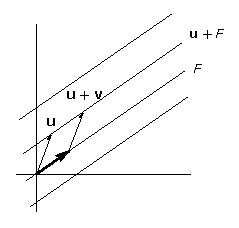
\includegraphics[width=2.5175in]{img/espvec-4.png}
\end{center}
\end{exemple}

\section{Rang d’un sistema de vectors}

\begin{definicio}
S’anomena \textbf{rang} d’un sistema $\mathcal{S}=(\mathbf{v}_{1},...,%
\mathbf{v}_{m})$ de $E$, denotat per $rang\,\mathcal{S}$, a la
dimensió de la clausura lineal d'aquest sistema, és a dir, en símbolos%
\begin{equation*}
rang\,\mathcal{S}=\dim \left\langle \mathbf{v}_{1},...,\mathbf{v}%
_{m}\right\rangle
\end{equation*}
\end{definicio}

\begin{observacio}
Dit d'una altra manera, el rang del sistema $(\mathbf{v}_{1},...,\mathbf{v}%
_{m}) $ és el nombre màxim de vectors linealment independents
que conté.
\end{observacio}

\begin{teorema}
Si $\mathcal{S}$ i $\mathcal{S}^{\prime }$ són dos sistema equivalents de $%
E$, aleshores%
\begin{equation*}
rang\,\mathcal{S}=rang\,\mathcal{S}^{\prime }
\end{equation*}

\end{teorema}
\begin{prova}
És una conseqüència immediata de la \textbf{definició 11}.
\end{prova}

\begin{corollari}
Donat un sistema $\mathcal{S}=(\mathbf{v}_{1},...,\mathbf{v}_{m})$, el seu rang
no varia si s'efectua qualsevol de les transformacions
elementals:

\begin{enumerate}
\item $rang\,\left( \mathbf{v}_{1},...,\mathbf{v}_{i},...,\mathbf{v}_{j},...%
\mathbf{v}_{m}\right) =rang\,\left( \mathbf{v}_{1},...,\mathbf{v}_{j},...,%
\mathbf{v}_{i},...\mathbf{v}_{m}\right) \,\ (i\neq j)$

\item $rang\,\left( \mathbf{v}_{1},...,\mathbf{v}_{i},...\mathbf{v}%
_{m}\right) =rang\,\left( \mathbf{v}_{1},...,\lambda \mathbf{v}_{i},...%
\mathbf{v}_{m}\right) $ $(\lambda \neq 0)$

\item $rang\,\left( \mathbf{v}_{1},...,\mathbf{v}_{i},...,\mathbf{v}_{j},...%
\mathbf{v}_{m}\right) =rang\,\left( \mathbf{v}_{1},...,\mathbf{v}%
_{i}+\lambda \mathbf{v}_{j},...,\mathbf{v}_{j},...\mathbf{v}_{m}\right) \,\
(i\neq j)$
\end{enumerate}

\end{corollari}
\begin{prova}
Estos resultats són conseqüèncias del \textbf{teorema 13}.
\end{prova}

\begin{corollari}
Donat un sistema $\mathcal{S}=(\mathbf{v}_{1},...,\mathbf{v}_{m})$, aleshores 
\begin{equation*}
rang\,(\mathbf{v}_{1},...,\mathbf{v}_{m})=rang\,(\mathbf{v}_{1},...,\mathbf{v%
}_{m},\mathbf{w})
\end{equation*}%
si i només si $\mathbf{w}$ és combinació lineal dels vectors de $(%
\mathbf{v}_{1},...,\mathbf{v}_{m})$.

\end{corollari}
\begin{prova}
És una conseqüència immediata del \textbf{teorema 12}.
\end{prova}

\begin{observacio}
Aquest darrer resultat permet assegurar que el rang d’un sistema no varia quan suprimim els vectors que són dependents dels
restants; en particular, podem suprimir els vectors nuls, i dels
vectors repetits, ens quedem només amb un d'ells.
\end{observacio}

\begin{teorema}
Donat un sistema de $r$ vectors $(\mathbf{u}_{1},...,\mathbf{u}_{r})$ d’un
espai vectorial $E$ de dimensió $n$ ($r\leq n$) i $(\mathbf{v%
}_{1},...,\mathbf{v}_{n})$ una base de $E$. Si expressem aquests
vectors en aquesta base 
\begin{equation*}
\mathbf{u}_{i}=\sum_{j=1}^{n}\lambda _{ij}\mathbf{v}_{j}\text{ \ \ }%
(i=1,...,r)
\end{equation*}
i es compleix%
\begin{equation*}
\lambda _{ij}=0\text{ per a }j<i
\end{equation*}%
i%
\begin{equation*}
\lambda _{ii}\neq 0\text{ per a tot }i=1,...,r
\end{equation*}%
aleshores $(\mathbf{u}_{1},...,\mathbf{u}_{r})$ és un sistema lliure.

\end{teorema}
\begin{prova}
Considerem%
\begin{equation*}
\mu _{1}\mathbf{u}_{1}+\cdots +\mu _{r}\mathbf{u}_{r}=\mathbf{0}
\end{equation*}%
Introduint les coordenades dels vectors en la base es té%
\begin{equation*}
\mu _{1}\sum_{j=1}^{n}\lambda _{1j}\mathbf{v}_{j}+\cdots +\mu
_{r}\sum_{j=1}^{n}\lambda _{rj}\mathbf{v}_{j}=\mathbf{0}
\end{equation*}%
D’aquí, com que $(\mathbf{v}_{1},...,\mathbf{v}_{n})$ és lliure, es
s’obtenen%
\begin{equation*}
\sum_{i=1}^{r}\mu _{i}\lambda _{ij}=\mathbf{0}\text{ \ \ }(j=1,...,n)
\end{equation*}%
Si ara tenim en compte les propietats de les $\lambda _{ij}$, obtenim:%
\begin{align*}
\mu _{1}\lambda _{11} &=0 \\
\mu _{1}\lambda _{12}+\mu _{2}\lambda _{22} &=0 \\
\mu _{1}\lambda _{13}+\mu _{2}\lambda _{23}+\mu _{3}\lambda _{33} &=0 \\
&&\vdots \\
\mu _{1}\lambda _{1r}+\mu _{2}\lambda _{2r}+\cdots +\mu _{r}\lambda _{rr}
&=0
\end{align*}%
és a dir, $\mu _{1}=\mu _{2}=\cdots =\mu _{r}=0$.
\end{prova}

\begin{observacio}
El teorema anterior ens dona un mètode per determinar el rang d’un
sistema. Per veure-ho, examina amb detall el següent exemple.
\end{observacio}

\begin{exemple}
En $\mathbb{R}^{4}$ determineu el rang del sistema $\mathcal{S}=(\mathbf{v}%
_{1},\mathbf{v}_{2},\mathbf{v}_{3},\mathbf{v}_{4})$, essent $\mathbf{v}%
_{1}=(1,1,2,0),\mathbf{v}_{2}=(1,1,0,6),\mathbf{v}_{3}=(-1,2,0,1),\mathbf{v}%
_{4}=(1,1,1,3)$.

\end{exemple}
\begin{solucio}
Prenent la base canònica de $\mathbb{R}^{4}$, escrivim les coordenades
d’aquests vectors per files (de la mateixa manera es faria per columnes) com
segueix:%
\begin{equation*}
\begin{tabular}{rrrrr}
$\mathbf{v}_{1}:$ & $1$ & $1$ & $2$ & $0$ \\ 
$\mathbf{v}_{2}:$ & $1$ & $1$ & $0$ & $6$ \\ 
$\mathbf{v}_{3}:$ & $-1$ & $2$ & $0$ & $1$ \\ 
$\mathbf{v}_{4}:$ & $1$ & $1$ & $1$ & $3$%
\end{tabular}%
\end{equation*}%
aplicant 3 vegades T3 s’obté%
\begin{equation*}
\begin{tabular}{rrrrr}
$v_{1}:$ & $1$ & $1$ & $2$ & $0$ \\ 
$v_{2}-v_{1}:$ & $0$ & $0$ & $-2$ & $6$ \\ 
$v_{3}+v_{1}:$ & $0$ & $3$ & $2$ & $1$ \\ 
$v_{4}-v_{1}:$ & $0$ & $0$ & $-1$ & $3$%
\end{tabular}%
\end{equation*}%
aplicant ara 2 vegades T1 s’obté%
\begin{equation*}
\begin{tabular}{rrrrr}
$\mathbf{v}_{1}:$ & $1$ & $1$ & $2$ & $0$ \\ 
$\mathbf{v}_{3}+\mathbf{v}_{1}:$ & $0$ & $3$ & $2$ & $1$ \\ 
$\mathbf{v}_{4}-\mathbf{v}_{1}:$ & $0$ & $0$ & $-1$ & $3$ \\ 
$\mathbf{v}_{2}-\mathbf{v}_{1}:$ & $0$ & $0$ & $-2$ & $6$%
\end{tabular}%
\end{equation*}%
aplicant una vez T3 s’obté%
\begin{equation*}
\begin{tabular}{rrrrr}
$\mathbf{v}_{1}:$ & $1$ & $1$ & $2$ & $0$ \\ 
$\mathbf{v}_{3}+\mathbf{v}_{1}:$ & $0$ & $3$ & $2$ & $1$ \\ 
$\mathbf{v}_{4}-\mathbf{v}_{1}:$ & $0$ & $0$ & $-1$ & $3$ \\ 
$\mathbf{v}_{2}-\mathbf{v}_{1}-2(\mathbf{v}_{4}-\mathbf{v}_{1}):$ & $0$ & $0$
& $0$ & $0$%
\end{tabular}%
\end{equation*}%
finalment, suprimint el vector nul es té%
\begin{equation*}
\begin{tabular}{rrrrr}
$\mathbf{v}_{1}:$ & $1$ & $1$ & $2$ & $0$ \\ 
$\mathbf{v}_{3}+\mathbf{v}_{1}:$ & $0$ & $3$ & $2$ & $1$ \\ 
$\mathbf{v}_{4}-\mathbf{v}_{1}:$ & $0$ & $0$ & $-1$ & $3$%
\end{tabular}%
\end{equation*}%
D’aquesta manera tenim%
\begin{equation*}
(\mathbf{v}_{1},\mathbf{v}_{2},\mathbf{v}_{3},\mathbf{v}_{4})\sim (\mathbf{v}%
_{1},\mathbf{v}_{3}+\mathbf{v}_{1},\mathbf{v}_{4}-\mathbf{v}_{1})
\end{equation*}%
Per tant,%
\begin{equation*}
rang\,(\mathbf{v}_{1},\mathbf{v}_{2},\mathbf{v}_{3},\mathbf{v}_{4})=rang\,(%
\mathbf{v}_{1},\mathbf{v}_{3}+\mathbf{v}_{1},\mathbf{v}_{4}-\mathbf{v}_{1})
\end{equation*}%
El sistema $(\mathbf{v}_{1},\mathbf{v}_{3}+\mathbf{v}_{1},\mathbf{v}_{4}-%
\mathbf{v}_{1})$ a més és lliure, ja que compleix les coordenades d’aquests
vectors compleixen les condicions del teorema anterior. Per tant,%
\begin{equation*}
rang(\mathbf{v}_{1},\mathbf{v}_{2},\mathbf{v}_{3},\mathbf{v}_{4})=rang(%
\mathbf{v}_{1},\mathbf{v}_{3}+\mathbf{v}_{1},\mathbf{v}_{4}-\mathbf{v}_{1})=3
\end{equation*}%
Com a conseqüèncial sistema donat $(\mathbf{v}_{1},\mathbf{v}_{2},\mathbf{v}%
_{3},\mathbf{v}_{4})$ és lligat. A més, a partir de les
transformacions aplicades anteriorment deduïm una relació de
dependència%
\begin{equation*}
\mathbf{v}_{2}-\mathbf{v}_{1}-2(\mathbf{v}_{4}-\mathbf{v}_{1})=\mathbf{0}
\end{equation*}%
és a dir%
\begin{equation*}
\mathbf{v}_{1}+\mathbf{v}_{2}-2\mathbf{v}_{4}=\mathbf{0}
\end{equation*}%
En general, comprovarem que el mètode ens dona no només el rang $s$
del sistema $(\mathbf{v}_{1},...,\mathbf{v}_{r})$, és a dir, la dimensió del subespai generat, sino també una base d’aquest subespai i
les $r-s$ relacions de dependència existeixentes entre els vectors del
sistema. En particular, si $E$ és de dimensió $n$ i $(\mathbf{v%
}_{1},...,\mathbf{v}_{n})$ és una base, aquest mètode permet calculeu les
coordenades d’un vector qualsevol respecte d'aquesta base.
\end{solucio}

\section{Isomorfismes d’espais vectorials}

\begin{definicio}
Donats dos espais vectorials $E$ i $E^{\prime }$ sobre
el mateix cos $\mathbb{K}$. S’anomena \textbf{isomorfisme} de $E$
en $E^{\prime }$ a tota aplicació bijectiva $f:E%
\rightarrow E^{\prime }$ que compleix:

\begin{enumerate}
\item Per a tot $\mathbf{u},\mathbf{v}\in E$, $f(\mathbf{u}+\mathbf{%
v})=f(\mathbf{u})+f(\mathbf{v})$

\item Per a tot $\mathbf{u}\in E$ i $\lambda \in \mathbb{K}$, $%
f(\lambda \mathbf{u})=\lambda f(\mathbf{u})$
\end{enumerate}

Si existeix un isomorfisme de $E$ en $E^{\prime }$, aleshores
es diu que $E$ i $E^{\prime }$ són dos espais
vectorials \textbf{isomorfs}. Escriurem aleshores%
\begin{equation*}
E\cong E^{\prime }
\end{equation*}
\end{definicio}

\begin{observacio}
Fem les observacions següents:

\begin{enumerate}
\item Afirmar que dos espais vectorials són isomorfs equival a dir
que tots dos tenen la mateixa estructura d’espai vectorial.

\item Estudiarem amb detall els isomorfismes com cas particular dels
homomorfismes d’espais vectorials (o aplicacions lineals) més
endavant en la secció corresponent.
\end{enumerate}
\end{observacio}

\begin{teorema}
Si $E_{1}$ i $E_{2}$ són dos subespais suplementaris de
un espai vectorial $E$, aleshores els espais $E=E%
_{1}\oplus E_{2}$ i $E_{1}\times E_{2}$ són
isomorfs.

\end{teorema}
\begin{prova}
Si $E_{1}$ i $E_{2}$ són dos subespais suplementaris de 
$E$, aleshores $E=E_{1}\oplus E_{2}$.
Considerem la descomposició única de tot $\mathbf{v}\in E$ com%
\begin{equation*}
\mathbf{v}=\mathbf{v}_{1}+\mathbf{v}_{2}
\end{equation*}%
amb $\mathbf{v}_{1}\in E_{1}$ i $\mathbf{v}_{2}\in E_{2}$.
Considerem l’aplicació $f$ de $E_{1}\times E_{2}$
en $E_{1}\oplus E_{2}$ definida per%
\begin{equation*}
f(\mathbf{v}_{1},\mathbf{v}_{2})=\mathbf{v}_{1}+\mathbf{v}_{2}
\end{equation*}%
Per construcció, és clar que $f$ és bijectiva. A més es compleix%
\begin{align*}
f\left( (\mathbf{v}_{1},\mathbf{v}_{2})+(\mathbf{w}_{1},\mathbf{w}%
_{2})\right) &=f(\mathbf{v}_{1}+\mathbf{w}_{1},\mathbf{v}_{2}+\mathbf{w}%
_{2})= \\
&=\left( \mathbf{v}_{1}+\mathbf{w}_{1}\right) +(\mathbf{v}_{2}+\mathbf{w}%
_{2})= \\
&=(\mathbf{v}_{1}+\mathbf{v}_{2})+(\mathbf{w}_{1}+\mathbf{w}_{2})= \\
&=f(\mathbf{v}_{1},\mathbf{v}_{2})+f(\mathbf{w}_{1},\mathbf{w}_{2})
\end{align*}%
i%
\begin{align*}
f(\lambda (\mathbf{v}_{1},\mathbf{v}_{2})) &=f(\lambda \mathbf{v}%
_{1},\lambda \mathbf{v}_{2})= \\
&=\lambda \mathbf{v}_{1}+\lambda \mathbf{v}_{2}= \\
&=\lambda (\mathbf{v}_{1}+\mathbf{v}_{2})= \\
&=\lambda f(\mathbf{v}_{1},\mathbf{v}_{2})
\end{align*}%
Per consegüent, $f$ és un isomorfisme.
\end{prova}

\begin{observacio}
Si $E_{1}$ i $E_{2}$ són dos espais vectorials sobre $%
\mathbb{K}$, podem construir un nou espai vectorial $E$ que
els contingui tots dos llevat d'un isomorfisme. En efecte, considerem
l'espai vectorial producte $E_{1}\times E_{2}$. Tot
vector $(\mathbf{v}_{1},\mathbf{v}_{2})$ de l’espai producte $E%
_{1}\times E_{2}$ pot descompondre's com segueix de manera única%
\begin{equation*}
(\mathbf{v}_{1},\mathbf{v}_{2})=(\mathbf{v}_{1},\mathbf{0})+(0,\mathbf{v}%
_{2})
\end{equation*}%
Considerem ara els dos subespais següents de $E_{1}\times 
E_{2}$: 
\begin{equation*}
E_{1}^{\prime }=\{(\mathbf{v}_{1},\mathbf{0}):\mathbf{v}_{1}\in 
E_{1}\}
\end{equation*}%
i 
\begin{equation*}
E_{2}^{\prime }=\{(\mathbf{0},\mathbf{v}_{2}):\mathbf{v}_{2}\in 
E_{2}\}
\end{equation*}%
És evident que $E_{1}\times E_{2}=E_{1}^{\prime
}\oplus E_{2}^{\prime }$, ja que els dos subespais tenen
intersecció $\{(\mathbf{0},\mathbf{0})\}$.

D’altra banda, és immediat comprovar que les aplicacions, $f_{1}:E_{1}^{\prime }\,\rightarrow \,E_{1}$ definida per $f_{1}(\mathbf{v}%
_{1},\mathbf{0})=\mathbf{v}_{1}$, i $f_{2}:E_{2}^{\prime
}\,\rightarrow \,E_{2}$ definida per $f_{2}(\mathbf{0},\mathbf{v}%
_{2})=\mathbf{v}_{2}$, són isomorfismes d’espais vectorials.

Com a conseqüència d’això, en la pràctica s'identifica sempre $E_{i}$ i $E_{i}^{\prime }$ ($i=1,2$); identificar per exemple $%
E_{1}$ i $E_{1}^{\prime }$ vol dir, confondre els
vectors $\mathbf{v}_{1}\in E_{1}$ i $(\mathbf{v}_{1},\mathbf{0}%
)\in E_{1}^{\prime }$. Aquesta identificació permet dir que $%
E_{1}$ i $E_{2}$ són subespais suplementaris de $%
E_{1}\times E_{2}$ . Pel teorema, els espais $E_{1}\times E_{2}$ i $E_{1}\oplus E_{2}$ són
isomorfs. \newline

L'espai $E=E_{1}\oplus E_{2}$ s’anomena \textbf{%
suma directa dels espais vectorials} donats $E_{1}$ i $E_{2}$. Aleshores, és clar que $E$ té $E_{1}$ i $%
E_{2}$ com a subespais suplementaris i es compleix que $E$
i $E_{1}\times E_{2}$ són isomorfs.

En aquestes condicions, si $\mathbf{v}\in E$, la descomposició 
única $\mathbf{v}=\mathbf{v}_{1}+\mathbf{v}_{2}$, fa que l'aplicació de $E$ en $E_{i}$ definida per 
\begin{equation*}
\begin{array}{lclcl}
\mathbf{v} & = & \mathbf{v}_{1}+\mathbf{v}_{2} & \longmapsto & \mathbf{v}_{i}%
\end{array}%
\end{equation*}%
s'identifica amb l’aplicació de $E_{1}\times E_{2}$
en $E_{i}$, que s’anomena la \textbf{\ projecció} $\pi _{i}$ de 
$E_{1}\times E_{2}$ sobre $E_{i}$ ($i=1,2$). Per
exemple, $\pi _{1}$ s’anomena \textbf{projecció de} $E$ \textbf{%
sobre el subespai} $E_{1}$ \textbf{paral·lelament al subespai} $%
E_{2}$, suplementari de $E_{1}$ respecte de $E$.
Es diu també que $\mathbf{v}_{1}$ (resp. $\mathbf{v}_{2}$) és la 
\textbf{component de} $\mathbf{v}$ de $E$ \textbf{en} $E%
_{1}$ (resp. $E_{2}$).
\end{observacio}

\begin{exemple}
Proveu que els espais vectorials següents $\mathbb{R}\oplus \mathbb{R}$
i $\mathbb{R}^{2}$ són isomorfs.

\end{exemple}
\begin{solucio}
Si prenem $E_{1}=E_{2}=\mathbb{R}$. Segons la observació anterior, podem afirmar que els espais vectorials reals $%
\mathbb{R}\oplus \mathbb{R}$ i $\mathbb{R}^{2}$ són isomorfs. Si
representem els elements de $E_{1}$ com els vectors de l'eix
real $Ox$, els de $E_{2}$ com els vectors de l'eix real $Oy$,
diferent de $Ox$, i els de $E_{1}\times E_{2}$ com els
vectors d'origen $O$ del pla ordinari, aleshores identificar $\mathbb{R}%
\oplus \mathbb{R}$ i $\mathbb{R}^{2}$ equival a confondre $(x_{1},y_{1})$
de $\mathbb{R}^{2}$ i $x_{1}+y_{1}$ de $\mathbb{R}\oplus \mathbb{R}$. La
figura següent il·lustra aquest fet.
\begin{center}
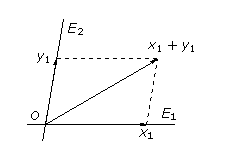
\includegraphics[width=2.3921in]{img/espvec-5.png}
\end{center}
\end{solucio}

\begin{teorema}
Si $E_{1}$ i $E_{2}$ són dos subespais suplementaris de
un espai vectorial $E$, aleshores l’espai quocient $E/%
E_{1}$ és isomorfo a $E_{2}$.

\end{teorema}
\begin{prova}
Si $E_{1}$ i $E_{2}$ són dos subespais suplementaris de
un espai vectorial $E$, aleshores $E=E_{1}\oplus 
E_{2}$. Donats $\mathbf{v}=\mathbf{v}_{1}+\mathbf{v}_{2}$ i $\mathbf{%
w}=\mathbf{w}_{1}+\mathbf{w}_{2}$ de $E$, la relació $\mathbf{v%
}_{1}+\mathbf{v}_{2}\equiv \mathbf{w}_{1}+\mathbf{w}_{2}$ (mod $E%
_{1}$) pot escriure’s com segueix%
\begin{equation*}
(\mathbf{v}_{1}+\mathbf{v}_{2})-(\mathbf{w}_{1}+\mathbf{w}_{2})=\mathbf{v}%
_{1}-\mathbf{w}_{1}+\mathbf{v}_{2}-\mathbf{w}_{2}\in E_{1}
\end{equation*}%
equivalent a $\mathbf{v}_{2}=\mathbf{w}_{2}$. Per tant, tots els vectors
d’una mateixa classe tenen la mateixa component en $E_{2}$.
Considerem l’aplicació $f:E/E_{1}\rightarrow 
E_{2}$ denida per%
\begin{equation*}
f(\left[ \mathbf{v}_{1}+\mathbf{v}_{2}\right] )=\mathbf{v}_{2}
\end{equation*}%
És clar que $f$ és exhaustiva, ja que qualsevol que sigui $\mathbf{v}_{2}$ de $%
E_{2}$ existeix $\left[ \mathbf{0}+\mathbf{v}_{2}\right] $ tal que $%
f\left( \left[ \mathbf{0}+\mathbf{v}_{2}\right] \right) =\mathbf{v}_{2}$.
A més, si 
\begin{equation*}
f\left( \left[ \mathbf{v}_{1}+\mathbf{v}_{2}\right] \right) =f\left( \left[ 
\mathbf{w}_{1}+\mathbf{w}_{2}\right] \right)
\end{equation*}%
aleshores $\mathbf{v}_{2}=\mathbf{w}_{2}$. Per tant,%
\begin{equation*}
(\mathbf{v}_{1}+\mathbf{v}_{2})-(\mathbf{w}_{1}+\mathbf{w}_{2})\in E%
_{1}
\end{equation*}%
és a dir,%
\begin{equation*}
\left[ \mathbf{v}_{1}+\mathbf{v}_{2}\right] =\left[ \mathbf{w}_{1}+\mathbf{w}%
_{2}\right]
\end{equation*}
Per tant, $f$ és inyectiva. Se compleix%
\begin{equation*}
f\left( \left[ \mathbf{v}\right] +\left[ \mathbf{w}\right] \right) =f\left( %
\left[ \mathbf{v}+\mathbf{w}\right] \right) =\mathbf{v}_{2}+\mathbf{w}%
_{2}=f\left( \left[ \mathbf{v}\right] \right) +f\left( \left[ \mathbf{w}%
\right] \right)
\end{equation*}%
i%
\begin{equation*}
f\left( \lambda \left[ \mathbf{v}\right] \right) =f\left( \left[ \lambda 
\mathbf{v}\right] \right) =\lambda \mathbf{v}_{2}=\lambda f\left( \left[ 
\mathbf{v}\right] \right)
\end{equation*}%
Per tant, $f$ és un isomorfisme.
\end{prova}

\begin{corollari}
En un espai vectorial $E$, tots els subespais suplementaris
d’un subespai vectorial $E_{1}$ de $E$ són isomorfs.

\end{corollari}
\begin{prova}
És una conseqüència immediata del teorema anterior.
\end{prova}

\begin{teorema}
Dos espais vectorials $E$ i $E^{\prime }$ de dimensió finita sobre
el mateix cos $K$ són isomorfs si i només si tenen la mateixa dimensió.

\end{teorema}
\begin{prova}
Suposem que $E$ i $E^{\prime }$ són de la mateixa dimensió $n$. Elegim una base $(\mathbf{v}_{1},...,\mathbf{v}_{n})$ de $%
E$ i una altra $(\mathbf{w}_{1},...,\mathbf{w}_{n})$ de $E%
^{\prime }$. Pel \textbf{teorema 15 (5)}, tot vector $\mathbf{u}\in 
E$ admet una expressió única com segueix%
\begin{equation*}
\mathbf{u}=\mu _{1}\mathbf{v}_{1}+\cdots +\mu _{n}\mathbf{v}_{n}
\end{equation*}%
Considerem l’aplicació $f$ de $E$ en $E^{\prime }$
definida per%
\begin{equation*}
f(\mathbf{u})=\mu _{1}\mathbf{w}_{1}+\cdots +\mu _{n}\mathbf{w}_{n}
\end{equation*}%
És clar que $f$ és bijectiva. D’altra banda, si $f(\mathbf{v})=\nu
_{1}w_{1}+\cdots +\nu _{n}w_{n}$, aleshores es compleix:%
\begin{align*}
f(\mathbf{u}+\mathbf{v}) &=\left( \mu _{1}+\nu _{1})w_{1}+\cdots +(\mu
_{n}+\nu _{n}\right) w_{n}= \\
&=(\mu _{1}w_{1}+\cdots +\mu _{n}w_{n})+(\nu _{1}w_{1}+\cdots +\nu
_{n}w_{n})= \\
&=f(\mathbf{u})+f(\mathbf{v})
\end{align*}%
i%
\begin{align*}
f(\lambda \mathbf{u}) &=\lambda \mu _{1}w_{1}+\cdots +\lambda \mu _{n}w_{n}=
\\
&=\lambda (\mu _{1}w_{1}+\cdots +\mu _{n}w_{n})= \\
&=\lambda f(\mathbf{u})
\end{align*}%
Per tant, aquesta aplicació és un isomorfisme de $E$ en $E^{\prime }$.

Recíprocament, suposem que $E$ i $E^{\prime }$
són isomorfs, i sigui $f$ el isomorfisme de $E$ en $E%
^{\prime }$. Suposem també que $\dim E=n$ i $\dim E^{\prime }=n^{\prime }$. Elegim una base $(\mathbf{v}_{1},...,\mathbf{v}%
_{n})$ de $E$. Denotem per $\mathbf{w}_{i}=f(\mathbf{v}_{i})$
per a cada $1\leq i\leq n$. Qualsevol vector $\mathbf{u}\in E$
admet una expressió única com segueix%
\begin{equation*}
\mathbf{u}=\mu _{1}\mathbf{v}_{1}+\cdots +\mu _{n}\mathbf{v}_{n}
\end{equation*}%
D’aquí, es té 
\begin{align*}
f(\mathbf{u)} &=f(\mu _{1}\mathbf{v}_{1}+\cdots +\mu _{n}\mathbf{v}_{n})= \\
&=\mu _{1}f(\mathbf{v}_{1})+\cdots +\mu _{n}f(\mathbf{v}_{n})= \\
&=\mu _{1}\mathbf{w}_{1}+\cdots +\mu _{n}\mathbf{w}_{n}
\end{align*}%
Com que $f$ és exhaustiva, qualsevol vector $\mathbf{w}\in E%
^{\prime }$ té una antiimagen en $E$. Suposem que $f(\mathbf{u%
})=\mathbf{w}$, aleshores%
\begin{equation*}
\mathbf{w}=\mu _{1}\mathbf{w}_{1}+\cdots +\mu _{n}\mathbf{w}_{n}
\end{equation*}%
Per tant, $(\mathbf{w}_{1},...,\mathbf{w}_{n})$ és un sistema generador de $%
E^{\prime }$. Veurem ara que $(\mathbf{w}_{1},...,\mathbf{w}%
_{n})$ és lliure. Per fer-ho, considerem%
\begin{equation*}
\lambda _{1}\mathbf{w}_{1}+\cdots +\lambda _{n}\mathbf{w}_{n}=\mathbf{0}
\end{equation*}%
és a dir%
\begin{equation*}
\lambda _{1}f(\mathbf{v}_{1})+\cdots +\lambda _{n}f(\mathbf{v}_{n})=\mathbf{0%
}
\end{equation*}%
D’aquí, segons la definició de isomorfisme, es dedueix%
\begin{equation*}
f(\lambda _{1}\mathbf{v}_{1}+\cdots +\lambda _{n}\mathbf{v}_{n})=f(\mathbf{0}%
)
\end{equation*}%
ja que 
\begin{equation*}
f(\mathbf{0})=f(\mathbf{0}+\mathbf{0})=f(\mathbf{0})+f(\mathbf{0})\text{ \ \
implica \ \ \ }f(\mathbf{0})=\mathbf{0}
\end{equation*}%
Ara bé, $f$ és inyectiva. Per tant,%
\begin{equation*}
\lambda _{1}\mathbf{v}_{1}+\cdots +\lambda _{n}\mathbf{v}_{n}=\mathbf{0}
\end{equation*}%
Com que $(\mathbf{v}_{1},...,\mathbf{v}_{n})$ és una base de $E$%
, es dedueix que $\lambda _{i}=0$ per a tot $1\leq i\leq n$. Per consegüent, 
$(\mathbf{w}_{1},...,\mathbf{w}_{n})$ és una base de $E^{\prime }$.
En conseqüència, els dos espais vectorials tenen la mateixa dimensió.
\end{prova}

\begin{observacio}
En la demostració d’aquest teorema es prova també que si dos
espais vectorials de dimensió finita són isomorfs, la aplicació transforma una base d’un en una base de l'altre. A més, el
isomorfisme queda perfectament definit un cop elegida una base de cada
espai vectorial. En concreto, el isomorfisme asocials vectors de les
mateixes coordenades.
\end{observacio}

\begin{corollari}
Tot espai vectorial $E$ de dimensió $n$ sobre $\mathbb{K}$
és isomorfo a $\mathbb{K}^{n}$.

\end{corollari}
\begin{prova}
El isomorfisme s’estableix una vez elegidas les bases: en $E$
escollim una base arbitrària $(\mathbf{v}_{1},...,\mathbf{v}_{n})$ i en $%
\mathbb{K}^{n}$ podem tomar la base natural $(\mathbf{e}_{1},...,\mathbf{e}%
_{n})$. Aleshores, el vector $\mathbf{v}=\lambda _{1}\mathbf{v}_{1}+\cdots
+\lambda _{n}\mathbf{v}_{n}$ de $E$ de coordenades $(\lambda
_{1},...,\lambda _{n})$ respecte de la base considerada es correspon amb
el vector $\mathbf{w}=\lambda _{1}\mathbf{e}_{1}+\cdots +\lambda _{n}\mathbf{%
e}_{n}$ de $\mathbb{K}^{n}$ de les mateixes coordenades en la base natural.
\end{prova}

\begin{observacio}
Després d’aquest darrer resultat, el estudi de $E$, des de
el punt de vista de la seva estructura vectorial, s'identifica així amb
l'estudi de $\mathbb{K}^{n}$ referit a la seva base natural. Aquesta és la raó
per la que s’anomena també \textbf{base canònica} a la base
natural de $\mathbb{K}^{n}$. Observeu que amb aquest resultat hem
resolt el problema de determinar (llevat d'isomorfisme) tots els espais
vectorials de dimensió finita.
\end{observacio}

\begin{corollari}
Donats dos espais vectorials $E_{1}$ i $E_{2}$ de
dimensions finites, aleshores es compleix 
\begin{equation*}
dim \,(E_{1}\times E_{2})=dim\,(E_{1}\oplus 
E_{2})=dim\,E_{1} + dim\,E_{2}
\end{equation*}

\end{corollari}
\begin{prova}
Segons la \textbf{observació 30} es té 
\begin{equation*}
E_{1}\times E_{2}\cong E_{1}\oplus E_{2}
\end{equation*}%
Per tant, pel \textbf{teorema 30}, tenim 
\begin{equation*}
dim\,(E_{1}\times E_{2})=dim\,(E_{1}\oplus 
E_{2})
\end{equation*}%
Per provar la darrera igualtat, suposem que $(\mathbf{v}_{1},...,%
\mathbf{v}_{n})$ i $(\mathbf{w}_{1},...,\mathbf{w}_{m})$ són bases de $%
E_{1}$ i $E_{2}$ respectivament. Aleshores és immediat
provar que 
\begin{equation*}
((\mathbf{v}_{1},\mathbf{0}),...,(\mathbf{v}_{n},\mathbf{0}),(\mathbf{0},%
\mathbf{w}_{1}),...,(\mathbf{0},\mathbf{w}_{m}))
\end{equation*}%
és una base de l’espai producte $E_{1}\times E_{2}$. Per
tanto 
\begin{equation*}
dim\,(E_{1}\times E_{2})=n+m
\end{equation*}
\end{prova}

\section{Canvi de coordenades}

\begin{definicio}
S’anomenan \textbf{coordenades d’un vector} $\mathbf{v}$ d’un espai
vectorial $E$ \textbf{respecte de la base} $(\mathbf{v}_{1},..., 
\mathbf{v}_{n})$ a la única família finita d'escalars $(\lambda
_{1},...,\lambda _{n})$ tals que%
\begin{equation*}
\mathbf{v}=\lambda _{1}\mathbf{v}_{1}+\cdots +\lambda _{n}\mathbf{v}_{n}
\end{equation*}
\end{definicio}

\begin{center}
\definecolor{figA}{HTML}{B02438}\definecolor{figB}{HTML}{27476E}%
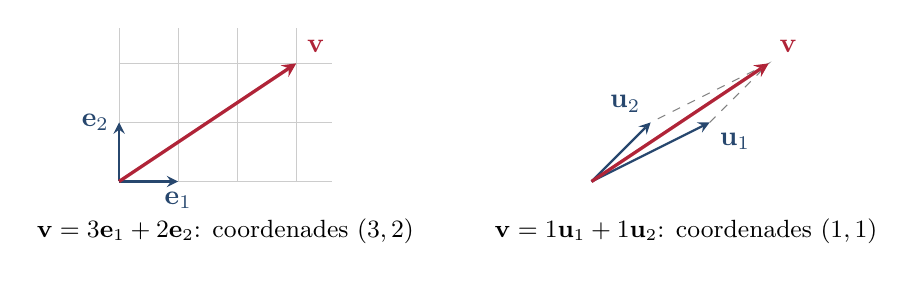
\begin{tikzpicture}[scale=0.75,>=stealth]
\draw[gray!40,very thin] (0,0) grid (3.6,2.6);
\draw[->,thick,figB] (0,0) -- (1,0) node[below]{$\mathbf{e}_{1}$};
\draw[->,thick,figB] (0,0) -- (0,1) node[left]{$\mathbf{e}_{2}$};
\draw[->,very thick,figA] (0,0) -- (3,2) node[above right]{$\mathbf{v}$};
\node at (1.8,-0.85) {\small $\mathbf{v}=3\mathbf{e}_{1}+2\mathbf{e}_{2}$: coordenades $(3,2)$};
\begin{scope}[xshift=8cm]
\draw[->,thick,figB] (0,0) -- (2,1) node[below right]{$\mathbf{u}_{1}$};
\draw[->,thick,figB] (0,0) -- (1,1) node[above left]{$\mathbf{u}_{2}$};
\draw[dashed,gray] (2,1) -- (3,2) -- (1,1);
\draw[->,very thick,figA] (0,0) -- (3,2) node[above right]{$\mathbf{v}$};
\node at (1.6,-0.85) {\small $\mathbf{v}=1\mathbf{u}_{1}+1\mathbf{u}_{2}$: coordenades $(1,1)$};
\end{scope}
\end{tikzpicture}

{\small\itshape Un mateix vector té coordenades diferents segons la base: $(3,2)$ en la base canònica i $(1,1)$ en la base $(\mathbf{u}_{1},\mathbf{u}_{2})$, amb $\mathbf{u}_{1}=(2,1)$ i $\mathbf{u}_{2}=(1,1)$.}
\end{center}

\begin{definicio}
Donat un espai vectorial $E$, en passar d’una base $\mathcal{B}%
_{1} $ a una base $\mathcal{B}_{2}$, diem que els vectors de $E$
\textbf{canvien} els seus \textbf{coordenades}. Es diu que el vector $\mathbf{v}$
té coordenades $(\lambda _{1},...,\lambda _{n})$ en $\mathcal{B}_{1}=(%
\mathbf{v}_{1},...,\mathbf{v}_{n})$ i $(\mu _{1},...,\mu _{n})$ en $\mathcal{%
B}_{2}=(\mathbf{u}_{1},...,\mathbf{u}_{n})$. La base $\mathcal{B}_{1}$ s'anomena \textbf{base antiga} i a $\mathcal{B}_{2}$, la \textbf{base nova}.

En el \textbf{teorema 31} s’indicarà com es calculen les
coordenades noves a partir de les antigues i recíprocament, i, en l’
\textbf{teorema 32} es donaran les equacions que caracteritzen la relació que hi ha entre les dues bases.
\end{definicio}

\begin{observacio}
Suposant $E=E^{\prime }$ en l’\textbf{teorema 30} i
elegint dues bases diferents $(\mathbf{v}_{1},...,\mathbf{v}_{n})$ i $(%
\mathbf{u}_{1},...,\mathbf{u}_{n})$ de $E$, l’aplicació
bijectiva que assigna a $\mathbf{v}=\lambda _{1}\mathbf{v}_{1}+\cdots
+\lambda _{n}\mathbf{v}_{n}$ el vector $\mathbf{w}=\lambda _{1}\mathbf{u}%
_{1}+\cdots +\lambda _{n}\mathbf{u}_{n}$, és un automorfisme de $E$
(un isomorfisme de $E$ en si mateix). Això fa que l'estudi
de $E$, realitzat utilitzant la base antiga, es conservi idènticament quan canviem de base i reemplacem els vectors estudiats
pels seus transformats en l'automorfisme associat, és a dir, els vectors
expressats en la base nova.
\end{observacio}

\begin{teorema}
Donades dues bases diferents $\mathcal{B}_{1}=(\mathbf{v}_{1},...,\mathbf{v}%
_{n})$ i $\mathcal{B}_{2}=(\mathbf{u}_{1},..., \mathbf{u}_{n})$ d’un
espai vectorial $E$. Sigui $\mathbf{v}$ un vector arbitrari de $%
E$ de coordenades $(\lambda _{1},...,\lambda _{n})$ en la base $%
\mathcal{B}_{1}$ i de coordenades $(\mu _{1},...,\mu _{n})$ en la base $%
\mathcal{B}_{2}$. Aleshores existeixen $n^{2}$ coeficients $\alpha _{ij}$ i $%
\beta_{ij}$ tals que 
\begin{equation*}
\lambda _{i}=\mu _{1}\alpha _{i1}+\cdots +\mu _{n}\alpha _{in}\text{ \ \ }
(i=1,...,n)
\end{equation*}%
i 
\begin{equation*}
\mu _{i}=\lambda _{1}\beta _{i1}+\cdots +\lambda _{n}\beta _{in}\text{ \ \ }
(i=1,...,n)
\end{equation*}

\end{teorema}
\begin{prova}
Sigui $\mathbf{v}$ un vector arbitrari de $E$ de coordenades $%
(\lambda _{1},...,\lambda _{n})$ en la base antiga $\mathcal{B}_{1}$.
Volem trobar les seves noves coordenades en la base nova $\mathcal{B}_{2}$.

Els vectors de la nova base estan definits per mitjà de les seves
coordenades en la base antiga per les equacions 
\begin{equation}
\mathbf{u}_{j}=\alpha _{1j}\mathbf{v}_{1}+\cdots +\alpha _{nj}\mathbf{v}_{n}%
\text{ \ \ \ }(j=1,...,n)  \label{1}
\end{equation}%
la qual cosa introdueix $n^{2}$ coeficients $\alpha _{ij}$. El vector $\mathbf{v}$
es descompon de dues maneres 
\begin{equation*}
\mathbf{v}=\lambda _{1}\mathbf{v}_{1}+\cdots +\lambda _{n}\mathbf{v}_{n}=\mu
_{1}\mathbf{u}_{1}+\cdots +\mu _{n}\mathbf{u}_{n}
\end{equation*}%
essent $(\mu _{1},...,\mu _{n})$ les coordenades noves de $\mathbf{v}$.
Reemplaçant els $\mathbf{u}_{j}$ de (1), s’obté 
\begin{equation*}
\lambda _{1}\mathbf{v}_{1}+\cdots +\lambda _{n}\mathbf{v}_{n}=\mu
_{1}(\alpha _{11}\mathbf{v}_{1}+\cdots +\alpha _{n1}\mathbf{v}_{n})+\cdots
+\mu _{n}(\alpha _{1n}\mathbf{v}_{1}+\cdots +\alpha _{nn}\mathbf{v}_{n})
\end{equation*}%
identificant en tots dos membres els coeficients de $\mathbf{v}_{j}$ es
té 
\begin{equation*}
\lambda _{i}=\mu _{1}\alpha _{i1}+\cdots +\mu _{n}\alpha _{in}\text{ \ \ }%
(i=1,...,n)
\end{equation*}

Aquestes són les expressions de les coordenades antigues en funció de les
noves.

Si es volen obtenir les fórmules inverses, n’hi ha prou d’escriure els vectors
de la base antiga per mitjà de les seves coordenades en la nova base%
\begin{equation}
\mathbf{v}_{j}=\beta _{1j}\mathbf{u}_{1}+\cdots +\beta _{nj}\mathbf{u}_{n}%
\text{ \ \ }(j=1,...,n)  \label{2}
\end{equation}%
i procedint de la mateixa manera s’obté 
\begin{equation*}
\mu _{i}=\lambda _{1}\beta _{i1}+\cdots +\lambda _{n}\beta _{in}\text{ \ \ }%
(i=1,...,n)
\end{equation*}
\end{prova}

\begin{observacio}
Podem escriure aquestes equacions d’una manera més còmoda
utilitzant matrius. Considerem les matrius següents 
\begin{equation*}
P=\left( 
\begin{array}{ccc}
\alpha _{11} & \cdots & \alpha _{1n} \\ 
\vdots & \ddots & \vdots \\ 
\alpha _{n1} & \cdots & \alpha _{nn}%
\end{array}%
\right) \,\,\ \ \ Q=\left( 
\begin{array}{ccc}
\beta _{11} & \cdots & \beta _{1n} \\ 
\vdots & \ddots & \vdots \\ 
\beta _{n1} & \cdots & \beta _{nn}%
\end{array}%
\right) \,\ \ \ A=\left( 
\begin{array}{c}
\lambda _{1} \\ 
\vdots \\ 
\lambda _{n}%
\end{array}%
\right) \,\ \ B=\left( 
\begin{array}{c}
\mu _{1} \\ 
\vdots \\ 
\mu _{n}%
\end{array}%
\right)
\end{equation*}%
Les equacions que relacionen les coordenades noves en $\mathcal{B}_{2}$ en
funció de les antigues en $\mathcal{B}_{1}$ es poden escriure així 
\begin{equation*}
B=QA
\end{equation*}%
i les equacions que relacionen les coordenades antigues en funció de
les noves com 
\begin{equation*}
A=PB
\end{equation*}

És important observar que les columnes de la matriu $P$ són els vectors de
la base nova $\mathcal{B}_{2}$ expressats en la base antiga $\mathcal{B}%
_{1}$. De la mateixa manera, les columnes de la matriu $Q$ són els vectors de la
base antiga $\mathcal{B}_{1}$ expressats en la base nova $\mathcal{B}_{2}$%
. Les matrius columna $A$ i $B$ són les coordenades d’un mateix vector
expressades en $\mathcal{B}_{1}$ i $\mathcal{B}_{2}$, respectivament

Les matrius $P$ i $Q$ s’anomenen \textbf{matrius de canvi de base}. També es diu que $P$ és la \textbf{matriu de pas} de la base nova $\mathcal{B}_{2}$ a la base antiga $\mathcal{B}_{1}$. De forma anàloga, $Q$ s’anomena matriu de pas de $\mathcal{B}_{1}$ a $\mathcal{B}_{2}$.
\end{observacio}

\begin{definicio}
Es defineix l’aplicació $\delta : \mathbb{N}_{n}\times \mathbb{N}%
_{n}\,\rightarrow\, \{0,1\}$ per 
\begin{equation*}
\delta (i,j)=\left\{ 
\begin{array}{l}
1\,\text{ si }\,i=j \\ 
0\,\text{ si }\,i\neq j%
\end{array}
\right.
\end{equation*}%
essent $\mathbb{N}_{n}=\{ 1,2,...,n\} $. El valor $\delta (i,j)$ es
es representa per $\delta _{ij}$ i rep el nom de \textbf{símbol de
Kronecker}.
\end{definicio}

\begin{teorema}
Donades dues bases diferents $(\mathbf{v}_{1},...,\mathbf{v}_{n})$ i $(\mathbf{u%
}_{1},...,\mathbf{u}_{n})$ d’un espai vectorial $E$. Les
coordenades $\alpha _{ij}$ i $\beta _{ij}$ dels vectors d’una base
l'una respecte de l'altra, estan lligades per les equacions característiques següents 
\begin{equation*}
\sum_{k=1}^{n}\alpha _{kj}\beta _{ik}=\delta _{ij}
\end{equation*}%
essent $\delta _{ij}$ el símbol de Kronecker.

\end{teorema}
\begin{prova}
En les equacions (1), introduint les equacions (2), s'obté 
\begin{equation*}
\mathbf{u}_{j}=(\alpha _{1j}\beta _{11}+\cdots +\alpha _{nj}\beta _{1n})%
\mathbf{u}_{1}+\cdots +(\alpha _{1j}\beta _{n1}+\cdots +\alpha _{nj}\beta
_{nn})\mathbf{u}_{n}
\end{equation*}%
\begin{align*}
\mathbf{u}_{j} &=\left( \sum_{k=1}^{n}\alpha _{kj}\beta _{1k}\right) 
\mathbf{u}_{1}+\cdots +\left( \sum_{k=1}^{n}\alpha _{kj}\beta _{nk}\right) 
\mathbf{u}_{n}= \\
&=\sum_{i=1}^{n}\sum_{k=1}^{n}\alpha _{kj}\beta _{ik}\mathbf{u}_{i}
\end{align*}%
Donat que $(\mathbf{u}_{1},...,\mathbf{u}_{n})$ és un sistema lliure, es
dedueixen les següents relacions:

\begin{enumerate}
\item Si $j=i$, el coeficient de $\mathbf{u}_{i}$ en el segon membre
ha de ser igual a $1$. Per tant, 
\begin{equation*}
\sum_{k=1}^{n}\alpha _{ki}\beta _{ik}=1\text{ \ \ \ }(i=1,...,n)
\end{equation*}

\item Si $j=r\neq i$, el coeficient de $\mathbf{u}_{r}$ en el segon
membre ha de ser igual a $0$. Per tant, 
\begin{equation*}
\sum_{k=1}^{n}\alpha _{kr}\beta _{ik}=0\text{ \ \ }(i=1,...,r-1,r+1,...,n)
\end{equation*}
\end{enumerate}

Introduint el símbol de Kronecker, les dues relacions anteriors s'escriuen en una sola com segueix 
\begin{equation*}
\sum_{k=1}^{n}\alpha _{kj}\beta _{ik}=\delta _{ij}
\end{equation*}
\end{prova}

\begin{observacio}
El teorema pot escriure’s més còmodament utilitzant matrius. En
efecte, observeu que la matriu associada a l’aplicació que defineix
el símbol de Kronecker per 
\begin{equation*}
a_{ij}=\delta _{ij}
\end{equation*}%
és la matriu que anomenem \textbf{matriu identitat d’ordre} $n$ que la
denotem per $I_{n}$ 
\begin{equation*}
I_{n}=\left( 
\begin{array}{cccc}
1 & 0 & \cdots & 0 \\ 
0 & 1 & \cdots & 0 \\ 
\vdots & \vdots & \ddots & \vdots \\ 
0 & 0 & \cdots & 1%
\end{array}%
\right)
\end{equation*}%
Les equacions anteriors s’escriuen així 
\begin{equation*}
QP=I_{n}
\end{equation*}%
Observeu que les matrius dels canvis de base són sempre
invertibles. De la darrera igualtat es dedueix 
\begin{equation*}
P=Q^{-1}\text{ \ \ \ \ i \ \ \ \ \ }Q=P^{-1}
\end{equation*}
\end{observacio}

\begin{exemple}
En $\mathbb{R}^{3}$ es consideren les bases $\mathcal{B}_{1}=(\mathbf{e}_{1},%
\mathbf{e}_{2},\mathbf{e}_{3})$ i $\mathcal{B}_{2}=(\mathbf{v}_{1},\mathbf{v}%
_{2},\mathbf{v}_{3})$ essent $\mathbf{v}_{1}=2\mathbf{e}_{1},\mathbf{v}_{2}=-%
\mathbf{e}_{2}+2\mathbf{e}_{3}$ i $\mathbf{v}_{3}=-3\mathbf{e}_{3}$. Trobeu
les coordenades respecte de $\mathcal{B}_{2}$ del vector $\mathbf{u}=4\mathbf{%
e}_{1}+\mathbf{e}_{2}-5\mathbf{e}_{3}$.

\end{exemple}
\begin{solucio}
Segons la \textbf{observació 34}, sabem que la matriu de canvi de
base o de pas de $\mathcal{B}_{2}$ a $\mathcal{B}_{1}$ té per vectors
columna als $\mathbf{v}_{i}$ referits a la base antiga $\mathcal{B}_{1}$%
. En aquest cas tenim%
\begin{equation*}
P=\left( 
\begin{array}{ccc}
2 & 0 & 0 \\ 
0 & -1 & 0 \\ 
0 & 2 & -3%
\end{array}%
\right)
\end{equation*}%
Aleshores, segons la \textbf{observació 35}, la matriu $Q$ de pas de 
$\mathcal{B}_{1}$ a $\mathcal{B}_{2}$ compleix%
\begin{equation*}
QP=I_{3}
\end{equation*}%
Per tant,%
\begin{equation*}
Q=P^{-1}=\frac{1}{6}\left( 
\begin{array}{ccc}
3 & 0 & 0 \\ 
0 & -6 & 0 \\ 
0 & -4 & -2%
\end{array}%
\right)
\end{equation*}%
Si $(x_{1},y_{1},z_{1})$ són les coordenades d’un vector referides a la
base $\mathcal{B}_{1}$ i $(x_{2},y_{2},z_{2})$ són les coordenades del mateix
vector referides a la base $\mathcal{B}_{2}$. Aleshores es compleix%
\begin{equation*}
\frac{1}{6}\left( 
\begin{array}{ccc}
3 & 0 & 0 \\ 
0 & -6 & 0 \\ 
0 & -4 & -2%
\end{array}%
\right) \left( 
\begin{array}{c}
x_{1} \\ 
y_{1} \\ 
z_{1}%
\end{array}%
\right) =\left( 
\begin{array}{c}
x_{2} \\ 
y_{2} \\ 
z_{2}%
\end{array}%
\right)
\end{equation*}%
Substituint les coordenades del vector $u$ es té%
\begin{equation*}
\frac{1}{6}\left( 
\begin{array}{ccc}
3 & 0 & 0 \\ 
0 & -6 & 0 \\ 
0 & -4 & -2%
\end{array}%
\right) \left( 
\begin{array}{c}
4 \\ 
1 \\ 
-5%
\end{array}%
\right) =\left( 
\begin{array}{c}
2 \\ 
-1 \\ 
1%
\end{array}%
\right)
\end{equation*}%
Per tant%
\begin{equation*}
\mathbf{u}=2\mathbf{v}_{1}-\mathbf{v}_{2}+\mathbf{v}_{3}
\end{equation*}
\end{solucio} 